The dataset will first be introduced in terms of its origin, content, and features, followed by an investigation into the distribution of action frequency within the dataset. Finally, a description will be provided of the baseline model proposed by the dataset creators, along with an account of the evaluation results.

\section{Introduction}
The Animal Kingdom dataset was proposed in CVPR 2022, which contains 50 hours of video clips with up to 850 unique species and 140 fine-grained classes of actions for action recognition. In addition, the footage provided is shot in diverse environmental conditions (e.g., grassland, forests, rivers, oceans) \parencite{ng2022animal}.

\section{Action Classes Frequency Distribution}

\begin{figure}[ht]
    \centering
    % 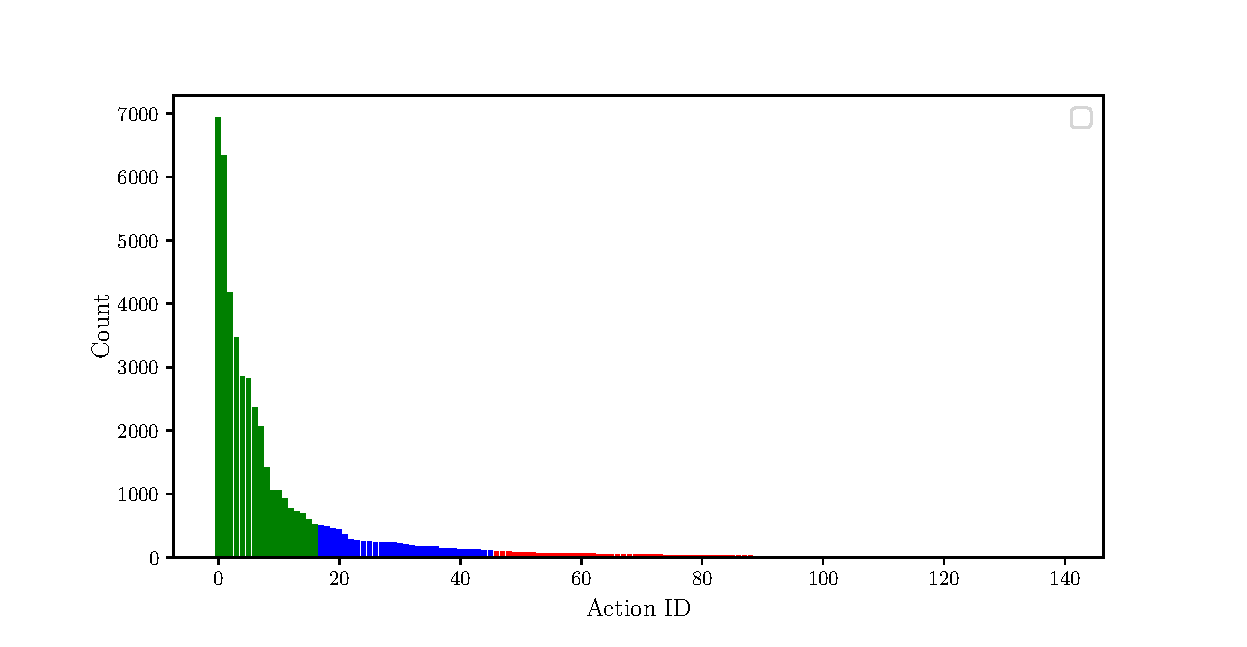
\includegraphics[width=1.0\textwidth]{assets/charts/4_1_LongTail}
    \resizebox{1.0\textwidth}{!}{%% Creator: Matplotlib, PGF backend
%%
%% To include the figure in your LaTeX document, write
%%   \input{<filename>.pgf}
%%
%% Make sure the required packages are loaded in your preamble
%%   \usepackage{pgf}
%%
%% Also ensure that all the required font packages are loaded; for instance,
%% the lmodern package is sometimes necessary when using math font.
%%   \usepackage{lmodern}
%%
%% Figures using additional raster images can only be included by \input if
%% they are in the same directory as the main LaTeX file. For loading figures
%% from other directories you can use the `import` package
%%   \usepackage{import}
%%
%% and then include the figures with
%%   \import{<path to file>}{<filename>.pgf}
%%
%% Matplotlib used the following preamble
%%
\begingroup%
\makeatletter%
\begin{pgfpicture}%
\pgfpathrectangle{\pgfpointorigin}{\pgfqpoint{8.000000in}{4.000000in}}%
\pgfusepath{use as bounding box, clip}%
\begin{pgfscope}%
\pgfsetbuttcap%
\pgfsetmiterjoin%
\definecolor{currentfill}{rgb}{1.000000,1.000000,1.000000}%
\pgfsetfillcolor{currentfill}%
\pgfsetlinewidth{0.000000pt}%
\definecolor{currentstroke}{rgb}{1.000000,1.000000,1.000000}%
\pgfsetstrokecolor{currentstroke}%
\pgfsetdash{}{0pt}%
\pgfpathmoveto{\pgfqpoint{0.000000in}{0.000000in}}%
\pgfpathlineto{\pgfqpoint{8.000000in}{0.000000in}}%
\pgfpathlineto{\pgfqpoint{8.000000in}{4.000000in}}%
\pgfpathlineto{\pgfqpoint{0.000000in}{4.000000in}}%
\pgfpathlineto{\pgfqpoint{0.000000in}{0.000000in}}%
\pgfpathclose%
\pgfusepath{fill}%
\end{pgfscope}%
\begin{pgfscope}%
\pgfsetbuttcap%
\pgfsetmiterjoin%
\definecolor{currentfill}{rgb}{1.000000,1.000000,1.000000}%
\pgfsetfillcolor{currentfill}%
\pgfsetlinewidth{0.000000pt}%
\definecolor{currentstroke}{rgb}{0.000000,0.000000,0.000000}%
\pgfsetstrokecolor{currentstroke}%
\pgfsetstrokeopacity{0.000000}%
\pgfsetdash{}{0pt}%
\pgfpathmoveto{\pgfqpoint{1.000000in}{0.440000in}}%
\pgfpathlineto{\pgfqpoint{7.200000in}{0.440000in}}%
\pgfpathlineto{\pgfqpoint{7.200000in}{3.520000in}}%
\pgfpathlineto{\pgfqpoint{1.000000in}{3.520000in}}%
\pgfpathlineto{\pgfqpoint{1.000000in}{0.440000in}}%
\pgfpathclose%
\pgfusepath{fill}%
\end{pgfscope}%
\begin{pgfscope}%
\pgfpathrectangle{\pgfqpoint{1.000000in}{0.440000in}}{\pgfqpoint{6.200000in}{3.080000in}}%
\pgfusepath{clip}%
\pgfsetbuttcap%
\pgfsetmiterjoin%
\definecolor{currentfill}{rgb}{0.000000,0.501961,0.000000}%
\pgfsetfillcolor{currentfill}%
\pgfsetlinewidth{0.000000pt}%
\definecolor{currentstroke}{rgb}{0.000000,0.000000,0.000000}%
\pgfsetstrokecolor{currentstroke}%
\pgfsetstrokeopacity{0.000000}%
\pgfsetdash{}{0pt}%
\pgfpathmoveto{\pgfqpoint{1.281818in}{0.440000in}}%
\pgfpathlineto{\pgfqpoint{1.314072in}{0.440000in}}%
\pgfpathlineto{\pgfqpoint{1.314072in}{3.373333in}}%
\pgfpathlineto{\pgfqpoint{1.281818in}{3.373333in}}%
\pgfpathlineto{\pgfqpoint{1.281818in}{0.440000in}}%
\pgfpathclose%
\pgfusepath{fill}%
\end{pgfscope}%
\begin{pgfscope}%
\pgfpathrectangle{\pgfqpoint{1.000000in}{0.440000in}}{\pgfqpoint{6.200000in}{3.080000in}}%
\pgfusepath{clip}%
\pgfsetbuttcap%
\pgfsetmiterjoin%
\definecolor{currentfill}{rgb}{0.000000,0.501961,0.000000}%
\pgfsetfillcolor{currentfill}%
\pgfsetlinewidth{0.000000pt}%
\definecolor{currentstroke}{rgb}{0.000000,0.000000,0.000000}%
\pgfsetstrokecolor{currentstroke}%
\pgfsetstrokeopacity{0.000000}%
\pgfsetdash{}{0pt}%
\pgfpathmoveto{\pgfqpoint{1.322136in}{0.440000in}}%
\pgfpathlineto{\pgfqpoint{1.354389in}{0.440000in}}%
\pgfpathlineto{\pgfqpoint{1.354389in}{3.119345in}}%
\pgfpathlineto{\pgfqpoint{1.322136in}{3.119345in}}%
\pgfpathlineto{\pgfqpoint{1.322136in}{0.440000in}}%
\pgfpathclose%
\pgfusepath{fill}%
\end{pgfscope}%
\begin{pgfscope}%
\pgfpathrectangle{\pgfqpoint{1.000000in}{0.440000in}}{\pgfqpoint{6.200000in}{3.080000in}}%
\pgfusepath{clip}%
\pgfsetbuttcap%
\pgfsetmiterjoin%
\definecolor{currentfill}{rgb}{0.000000,0.501961,0.000000}%
\pgfsetfillcolor{currentfill}%
\pgfsetlinewidth{0.000000pt}%
\definecolor{currentstroke}{rgb}{0.000000,0.000000,0.000000}%
\pgfsetstrokecolor{currentstroke}%
\pgfsetstrokeopacity{0.000000}%
\pgfsetdash{}{0pt}%
\pgfpathmoveto{\pgfqpoint{1.362453in}{0.440000in}}%
\pgfpathlineto{\pgfqpoint{1.394707in}{0.440000in}}%
\pgfpathlineto{\pgfqpoint{1.394707in}{2.206508in}}%
\pgfpathlineto{\pgfqpoint{1.362453in}{2.206508in}}%
\pgfpathlineto{\pgfqpoint{1.362453in}{0.440000in}}%
\pgfpathclose%
\pgfusepath{fill}%
\end{pgfscope}%
\begin{pgfscope}%
\pgfpathrectangle{\pgfqpoint{1.000000in}{0.440000in}}{\pgfqpoint{6.200000in}{3.080000in}}%
\pgfusepath{clip}%
\pgfsetbuttcap%
\pgfsetmiterjoin%
\definecolor{currentfill}{rgb}{0.000000,0.501961,0.000000}%
\pgfsetfillcolor{currentfill}%
\pgfsetlinewidth{0.000000pt}%
\definecolor{currentstroke}{rgb}{0.000000,0.000000,0.000000}%
\pgfsetstrokecolor{currentstroke}%
\pgfsetstrokeopacity{0.000000}%
\pgfsetdash{}{0pt}%
\pgfpathmoveto{\pgfqpoint{1.402770in}{0.440000in}}%
\pgfpathlineto{\pgfqpoint{1.435024in}{0.440000in}}%
\pgfpathlineto{\pgfqpoint{1.435024in}{1.904765in}}%
\pgfpathlineto{\pgfqpoint{1.402770in}{1.904765in}}%
\pgfpathlineto{\pgfqpoint{1.402770in}{0.440000in}}%
\pgfpathclose%
\pgfusepath{fill}%
\end{pgfscope}%
\begin{pgfscope}%
\pgfpathrectangle{\pgfqpoint{1.000000in}{0.440000in}}{\pgfqpoint{6.200000in}{3.080000in}}%
\pgfusepath{clip}%
\pgfsetbuttcap%
\pgfsetmiterjoin%
\definecolor{currentfill}{rgb}{0.000000,0.501961,0.000000}%
\pgfsetfillcolor{currentfill}%
\pgfsetlinewidth{0.000000pt}%
\definecolor{currentstroke}{rgb}{0.000000,0.000000,0.000000}%
\pgfsetstrokecolor{currentstroke}%
\pgfsetstrokeopacity{0.000000}%
\pgfsetdash{}{0pt}%
\pgfpathmoveto{\pgfqpoint{1.443088in}{0.440000in}}%
\pgfpathlineto{\pgfqpoint{1.475341in}{0.440000in}}%
\pgfpathlineto{\pgfqpoint{1.475341in}{1.646973in}}%
\pgfpathlineto{\pgfqpoint{1.443088in}{1.646973in}}%
\pgfpathlineto{\pgfqpoint{1.443088in}{0.440000in}}%
\pgfpathclose%
\pgfusepath{fill}%
\end{pgfscope}%
\begin{pgfscope}%
\pgfpathrectangle{\pgfqpoint{1.000000in}{0.440000in}}{\pgfqpoint{6.200000in}{3.080000in}}%
\pgfusepath{clip}%
\pgfsetbuttcap%
\pgfsetmiterjoin%
\definecolor{currentfill}{rgb}{0.000000,0.501961,0.000000}%
\pgfsetfillcolor{currentfill}%
\pgfsetlinewidth{0.000000pt}%
\definecolor{currentstroke}{rgb}{0.000000,0.000000,0.000000}%
\pgfsetstrokecolor{currentstroke}%
\pgfsetstrokeopacity{0.000000}%
\pgfsetdash{}{0pt}%
\pgfpathmoveto{\pgfqpoint{1.483405in}{0.440000in}}%
\pgfpathlineto{\pgfqpoint{1.515659in}{0.440000in}}%
\pgfpathlineto{\pgfqpoint{1.515659in}{1.634295in}}%
\pgfpathlineto{\pgfqpoint{1.483405in}{1.634295in}}%
\pgfpathlineto{\pgfqpoint{1.483405in}{0.440000in}}%
\pgfpathclose%
\pgfusepath{fill}%
\end{pgfscope}%
\begin{pgfscope}%
\pgfpathrectangle{\pgfqpoint{1.000000in}{0.440000in}}{\pgfqpoint{6.200000in}{3.080000in}}%
\pgfusepath{clip}%
\pgfsetbuttcap%
\pgfsetmiterjoin%
\definecolor{currentfill}{rgb}{0.000000,0.501961,0.000000}%
\pgfsetfillcolor{currentfill}%
\pgfsetlinewidth{0.000000pt}%
\definecolor{currentstroke}{rgb}{0.000000,0.000000,0.000000}%
\pgfsetstrokecolor{currentstroke}%
\pgfsetstrokeopacity{0.000000}%
\pgfsetdash{}{0pt}%
\pgfpathmoveto{\pgfqpoint{1.523722in}{0.440000in}}%
\pgfpathlineto{\pgfqpoint{1.555976in}{0.440000in}}%
\pgfpathlineto{\pgfqpoint{1.555976in}{1.440740in}}%
\pgfpathlineto{\pgfqpoint{1.523722in}{1.440740in}}%
\pgfpathlineto{\pgfqpoint{1.523722in}{0.440000in}}%
\pgfpathclose%
\pgfusepath{fill}%
\end{pgfscope}%
\begin{pgfscope}%
\pgfpathrectangle{\pgfqpoint{1.000000in}{0.440000in}}{\pgfqpoint{6.200000in}{3.080000in}}%
\pgfusepath{clip}%
\pgfsetbuttcap%
\pgfsetmiterjoin%
\definecolor{currentfill}{rgb}{0.000000,0.501961,0.000000}%
\pgfsetfillcolor{currentfill}%
\pgfsetlinewidth{0.000000pt}%
\definecolor{currentstroke}{rgb}{0.000000,0.000000,0.000000}%
\pgfsetstrokecolor{currentstroke}%
\pgfsetstrokeopacity{0.000000}%
\pgfsetdash{}{0pt}%
\pgfpathmoveto{\pgfqpoint{1.564040in}{0.440000in}}%
\pgfpathlineto{\pgfqpoint{1.596293in}{0.440000in}}%
\pgfpathlineto{\pgfqpoint{1.596293in}{1.309731in}}%
\pgfpathlineto{\pgfqpoint{1.564040in}{1.309731in}}%
\pgfpathlineto{\pgfqpoint{1.564040in}{0.440000in}}%
\pgfpathclose%
\pgfusepath{fill}%
\end{pgfscope}%
\begin{pgfscope}%
\pgfpathrectangle{\pgfqpoint{1.000000in}{0.440000in}}{\pgfqpoint{6.200000in}{3.080000in}}%
\pgfusepath{clip}%
\pgfsetbuttcap%
\pgfsetmiterjoin%
\definecolor{currentfill}{rgb}{0.000000,0.501961,0.000000}%
\pgfsetfillcolor{currentfill}%
\pgfsetlinewidth{0.000000pt}%
\definecolor{currentstroke}{rgb}{0.000000,0.000000,0.000000}%
\pgfsetstrokecolor{currentstroke}%
\pgfsetstrokeopacity{0.000000}%
\pgfsetdash{}{0pt}%
\pgfpathmoveto{\pgfqpoint{1.604357in}{0.440000in}}%
\pgfpathlineto{\pgfqpoint{1.636611in}{0.440000in}}%
\pgfpathlineto{\pgfqpoint{1.636611in}{1.037570in}}%
\pgfpathlineto{\pgfqpoint{1.604357in}{1.037570in}}%
\pgfpathlineto{\pgfqpoint{1.604357in}{0.440000in}}%
\pgfpathclose%
\pgfusepath{fill}%
\end{pgfscope}%
\begin{pgfscope}%
\pgfpathrectangle{\pgfqpoint{1.000000in}{0.440000in}}{\pgfqpoint{6.200000in}{3.080000in}}%
\pgfusepath{clip}%
\pgfsetbuttcap%
\pgfsetmiterjoin%
\definecolor{currentfill}{rgb}{0.000000,0.501961,0.000000}%
\pgfsetfillcolor{currentfill}%
\pgfsetlinewidth{0.000000pt}%
\definecolor{currentstroke}{rgb}{0.000000,0.000000,0.000000}%
\pgfsetstrokecolor{currentstroke}%
\pgfsetstrokeopacity{0.000000}%
\pgfsetdash{}{0pt}%
\pgfpathmoveto{\pgfqpoint{1.644674in}{0.440000in}}%
\pgfpathlineto{\pgfqpoint{1.676928in}{0.440000in}}%
\pgfpathlineto{\pgfqpoint{1.676928in}{0.887544in}}%
\pgfpathlineto{\pgfqpoint{1.644674in}{0.887544in}}%
\pgfpathlineto{\pgfqpoint{1.644674in}{0.440000in}}%
\pgfpathclose%
\pgfusepath{fill}%
\end{pgfscope}%
\begin{pgfscope}%
\pgfpathrectangle{\pgfqpoint{1.000000in}{0.440000in}}{\pgfqpoint{6.200000in}{3.080000in}}%
\pgfusepath{clip}%
\pgfsetbuttcap%
\pgfsetmiterjoin%
\definecolor{currentfill}{rgb}{0.000000,0.501961,0.000000}%
\pgfsetfillcolor{currentfill}%
\pgfsetlinewidth{0.000000pt}%
\definecolor{currentstroke}{rgb}{0.000000,0.000000,0.000000}%
\pgfsetstrokecolor{currentstroke}%
\pgfsetstrokeopacity{0.000000}%
\pgfsetdash{}{0pt}%
\pgfpathmoveto{\pgfqpoint{1.684992in}{0.440000in}}%
\pgfpathlineto{\pgfqpoint{1.717245in}{0.440000in}}%
\pgfpathlineto{\pgfqpoint{1.717245in}{0.884163in}}%
\pgfpathlineto{\pgfqpoint{1.684992in}{0.884163in}}%
\pgfpathlineto{\pgfqpoint{1.684992in}{0.440000in}}%
\pgfpathclose%
\pgfusepath{fill}%
\end{pgfscope}%
\begin{pgfscope}%
\pgfpathrectangle{\pgfqpoint{1.000000in}{0.440000in}}{\pgfqpoint{6.200000in}{3.080000in}}%
\pgfusepath{clip}%
\pgfsetbuttcap%
\pgfsetmiterjoin%
\definecolor{currentfill}{rgb}{0.000000,0.501961,0.000000}%
\pgfsetfillcolor{currentfill}%
\pgfsetlinewidth{0.000000pt}%
\definecolor{currentstroke}{rgb}{0.000000,0.000000,0.000000}%
\pgfsetstrokecolor{currentstroke}%
\pgfsetstrokeopacity{0.000000}%
\pgfsetdash{}{0pt}%
\pgfpathmoveto{\pgfqpoint{1.725309in}{0.440000in}}%
\pgfpathlineto{\pgfqpoint{1.757563in}{0.440000in}}%
\pgfpathlineto{\pgfqpoint{1.757563in}{0.830069in}}%
\pgfpathlineto{\pgfqpoint{1.725309in}{0.830069in}}%
\pgfpathlineto{\pgfqpoint{1.725309in}{0.440000in}}%
\pgfpathclose%
\pgfusepath{fill}%
\end{pgfscope}%
\begin{pgfscope}%
\pgfpathrectangle{\pgfqpoint{1.000000in}{0.440000in}}{\pgfqpoint{6.200000in}{3.080000in}}%
\pgfusepath{clip}%
\pgfsetbuttcap%
\pgfsetmiterjoin%
\definecolor{currentfill}{rgb}{0.000000,0.501961,0.000000}%
\pgfsetfillcolor{currentfill}%
\pgfsetlinewidth{0.000000pt}%
\definecolor{currentstroke}{rgb}{0.000000,0.000000,0.000000}%
\pgfsetstrokecolor{currentstroke}%
\pgfsetstrokeopacity{0.000000}%
\pgfsetdash{}{0pt}%
\pgfpathmoveto{\pgfqpoint{1.765626in}{0.440000in}}%
\pgfpathlineto{\pgfqpoint{1.797880in}{0.440000in}}%
\pgfpathlineto{\pgfqpoint{1.797880in}{0.763719in}}%
\pgfpathlineto{\pgfqpoint{1.765626in}{0.763719in}}%
\pgfpathlineto{\pgfqpoint{1.765626in}{0.440000in}}%
\pgfpathclose%
\pgfusepath{fill}%
\end{pgfscope}%
\begin{pgfscope}%
\pgfpathrectangle{\pgfqpoint{1.000000in}{0.440000in}}{\pgfqpoint{6.200000in}{3.080000in}}%
\pgfusepath{clip}%
\pgfsetbuttcap%
\pgfsetmiterjoin%
\definecolor{currentfill}{rgb}{0.000000,0.501961,0.000000}%
\pgfsetfillcolor{currentfill}%
\pgfsetlinewidth{0.000000pt}%
\definecolor{currentstroke}{rgb}{0.000000,0.000000,0.000000}%
\pgfsetstrokecolor{currentstroke}%
\pgfsetstrokeopacity{0.000000}%
\pgfsetdash{}{0pt}%
\pgfpathmoveto{\pgfqpoint{1.805944in}{0.440000in}}%
\pgfpathlineto{\pgfqpoint{1.838197in}{0.440000in}}%
\pgfpathlineto{\pgfqpoint{1.838197in}{0.748928in}}%
\pgfpathlineto{\pgfqpoint{1.805944in}{0.748928in}}%
\pgfpathlineto{\pgfqpoint{1.805944in}{0.440000in}}%
\pgfpathclose%
\pgfusepath{fill}%
\end{pgfscope}%
\begin{pgfscope}%
\pgfpathrectangle{\pgfqpoint{1.000000in}{0.440000in}}{\pgfqpoint{6.200000in}{3.080000in}}%
\pgfusepath{clip}%
\pgfsetbuttcap%
\pgfsetmiterjoin%
\definecolor{currentfill}{rgb}{0.000000,0.501961,0.000000}%
\pgfsetfillcolor{currentfill}%
\pgfsetlinewidth{0.000000pt}%
\definecolor{currentstroke}{rgb}{0.000000,0.000000,0.000000}%
\pgfsetstrokecolor{currentstroke}%
\pgfsetstrokeopacity{0.000000}%
\pgfsetdash{}{0pt}%
\pgfpathmoveto{\pgfqpoint{1.846261in}{0.440000in}}%
\pgfpathlineto{\pgfqpoint{1.878515in}{0.440000in}}%
\pgfpathlineto{\pgfqpoint{1.878515in}{0.733714in}}%
\pgfpathlineto{\pgfqpoint{1.846261in}{0.733714in}}%
\pgfpathlineto{\pgfqpoint{1.846261in}{0.440000in}}%
\pgfpathclose%
\pgfusepath{fill}%
\end{pgfscope}%
\begin{pgfscope}%
\pgfpathrectangle{\pgfqpoint{1.000000in}{0.440000in}}{\pgfqpoint{6.200000in}{3.080000in}}%
\pgfusepath{clip}%
\pgfsetbuttcap%
\pgfsetmiterjoin%
\definecolor{currentfill}{rgb}{0.000000,0.501961,0.000000}%
\pgfsetfillcolor{currentfill}%
\pgfsetlinewidth{0.000000pt}%
\definecolor{currentstroke}{rgb}{0.000000,0.000000,0.000000}%
\pgfsetstrokecolor{currentstroke}%
\pgfsetstrokeopacity{0.000000}%
\pgfsetdash{}{0pt}%
\pgfpathmoveto{\pgfqpoint{1.886578in}{0.440000in}}%
\pgfpathlineto{\pgfqpoint{1.918832in}{0.440000in}}%
\pgfpathlineto{\pgfqpoint{1.918832in}{0.694411in}}%
\pgfpathlineto{\pgfqpoint{1.886578in}{0.694411in}}%
\pgfpathlineto{\pgfqpoint{1.886578in}{0.440000in}}%
\pgfpathclose%
\pgfusepath{fill}%
\end{pgfscope}%
\begin{pgfscope}%
\pgfpathrectangle{\pgfqpoint{1.000000in}{0.440000in}}{\pgfqpoint{6.200000in}{3.080000in}}%
\pgfusepath{clip}%
\pgfsetbuttcap%
\pgfsetmiterjoin%
\definecolor{currentfill}{rgb}{0.000000,0.501961,0.000000}%
\pgfsetfillcolor{currentfill}%
\pgfsetlinewidth{0.000000pt}%
\definecolor{currentstroke}{rgb}{0.000000,0.000000,0.000000}%
\pgfsetstrokecolor{currentstroke}%
\pgfsetstrokeopacity{0.000000}%
\pgfsetdash{}{0pt}%
\pgfpathmoveto{\pgfqpoint{1.926896in}{0.440000in}}%
\pgfpathlineto{\pgfqpoint{1.959149in}{0.440000in}}%
\pgfpathlineto{\pgfqpoint{1.959149in}{0.655954in}}%
\pgfpathlineto{\pgfqpoint{1.926896in}{0.655954in}}%
\pgfpathlineto{\pgfqpoint{1.926896in}{0.440000in}}%
\pgfpathclose%
\pgfusepath{fill}%
\end{pgfscope}%
\begin{pgfscope}%
\pgfpathrectangle{\pgfqpoint{1.000000in}{0.440000in}}{\pgfqpoint{6.200000in}{3.080000in}}%
\pgfusepath{clip}%
\pgfsetbuttcap%
\pgfsetmiterjoin%
\definecolor{currentfill}{rgb}{0.000000,0.000000,1.000000}%
\pgfsetfillcolor{currentfill}%
\pgfsetlinewidth{0.000000pt}%
\definecolor{currentstroke}{rgb}{0.000000,0.000000,0.000000}%
\pgfsetstrokecolor{currentstroke}%
\pgfsetstrokeopacity{0.000000}%
\pgfsetdash{}{0pt}%
\pgfpathmoveto{\pgfqpoint{1.967213in}{0.440000in}}%
\pgfpathlineto{\pgfqpoint{1.999467in}{0.440000in}}%
\pgfpathlineto{\pgfqpoint{1.999467in}{0.650882in}}%
\pgfpathlineto{\pgfqpoint{1.967213in}{0.650882in}}%
\pgfpathlineto{\pgfqpoint{1.967213in}{0.440000in}}%
\pgfpathclose%
\pgfusepath{fill}%
\end{pgfscope}%
\begin{pgfscope}%
\pgfpathrectangle{\pgfqpoint{1.000000in}{0.440000in}}{\pgfqpoint{6.200000in}{3.080000in}}%
\pgfusepath{clip}%
\pgfsetbuttcap%
\pgfsetmiterjoin%
\definecolor{currentfill}{rgb}{0.000000,0.000000,1.000000}%
\pgfsetfillcolor{currentfill}%
\pgfsetlinewidth{0.000000pt}%
\definecolor{currentstroke}{rgb}{0.000000,0.000000,0.000000}%
\pgfsetstrokecolor{currentstroke}%
\pgfsetstrokeopacity{0.000000}%
\pgfsetdash{}{0pt}%
\pgfpathmoveto{\pgfqpoint{2.007530in}{0.440000in}}%
\pgfpathlineto{\pgfqpoint{2.039784in}{0.440000in}}%
\pgfpathlineto{\pgfqpoint{2.039784in}{0.645388in}}%
\pgfpathlineto{\pgfqpoint{2.007530in}{0.645388in}}%
\pgfpathlineto{\pgfqpoint{2.007530in}{0.440000in}}%
\pgfpathclose%
\pgfusepath{fill}%
\end{pgfscope}%
\begin{pgfscope}%
\pgfpathrectangle{\pgfqpoint{1.000000in}{0.440000in}}{\pgfqpoint{6.200000in}{3.080000in}}%
\pgfusepath{clip}%
\pgfsetbuttcap%
\pgfsetmiterjoin%
\definecolor{currentfill}{rgb}{0.000000,0.000000,1.000000}%
\pgfsetfillcolor{currentfill}%
\pgfsetlinewidth{0.000000pt}%
\definecolor{currentstroke}{rgb}{0.000000,0.000000,0.000000}%
\pgfsetstrokecolor{currentstroke}%
\pgfsetstrokeopacity{0.000000}%
\pgfsetdash{}{0pt}%
\pgfpathmoveto{\pgfqpoint{2.047848in}{0.440000in}}%
\pgfpathlineto{\pgfqpoint{2.080101in}{0.440000in}}%
\pgfpathlineto{\pgfqpoint{2.080101in}{0.635668in}}%
\pgfpathlineto{\pgfqpoint{2.047848in}{0.635668in}}%
\pgfpathlineto{\pgfqpoint{2.047848in}{0.440000in}}%
\pgfpathclose%
\pgfusepath{fill}%
\end{pgfscope}%
\begin{pgfscope}%
\pgfpathrectangle{\pgfqpoint{1.000000in}{0.440000in}}{\pgfqpoint{6.200000in}{3.080000in}}%
\pgfusepath{clip}%
\pgfsetbuttcap%
\pgfsetmiterjoin%
\definecolor{currentfill}{rgb}{0.000000,0.000000,1.000000}%
\pgfsetfillcolor{currentfill}%
\pgfsetlinewidth{0.000000pt}%
\definecolor{currentstroke}{rgb}{0.000000,0.000000,0.000000}%
\pgfsetstrokecolor{currentstroke}%
\pgfsetstrokeopacity{0.000000}%
\pgfsetdash{}{0pt}%
\pgfpathmoveto{\pgfqpoint{2.088165in}{0.440000in}}%
\pgfpathlineto{\pgfqpoint{2.120419in}{0.440000in}}%
\pgfpathlineto{\pgfqpoint{2.120419in}{0.623413in}}%
\pgfpathlineto{\pgfqpoint{2.088165in}{0.623413in}}%
\pgfpathlineto{\pgfqpoint{2.088165in}{0.440000in}}%
\pgfpathclose%
\pgfusepath{fill}%
\end{pgfscope}%
\begin{pgfscope}%
\pgfpathrectangle{\pgfqpoint{1.000000in}{0.440000in}}{\pgfqpoint{6.200000in}{3.080000in}}%
\pgfusepath{clip}%
\pgfsetbuttcap%
\pgfsetmiterjoin%
\definecolor{currentfill}{rgb}{0.000000,0.000000,1.000000}%
\pgfsetfillcolor{currentfill}%
\pgfsetlinewidth{0.000000pt}%
\definecolor{currentstroke}{rgb}{0.000000,0.000000,0.000000}%
\pgfsetstrokecolor{currentstroke}%
\pgfsetstrokeopacity{0.000000}%
\pgfsetdash{}{0pt}%
\pgfpathmoveto{\pgfqpoint{2.128482in}{0.440000in}}%
\pgfpathlineto{\pgfqpoint{2.160736in}{0.440000in}}%
\pgfpathlineto{\pgfqpoint{2.160736in}{0.591294in}}%
\pgfpathlineto{\pgfqpoint{2.128482in}{0.591294in}}%
\pgfpathlineto{\pgfqpoint{2.128482in}{0.440000in}}%
\pgfpathclose%
\pgfusepath{fill}%
\end{pgfscope}%
\begin{pgfscope}%
\pgfpathrectangle{\pgfqpoint{1.000000in}{0.440000in}}{\pgfqpoint{6.200000in}{3.080000in}}%
\pgfusepath{clip}%
\pgfsetbuttcap%
\pgfsetmiterjoin%
\definecolor{currentfill}{rgb}{0.000000,0.000000,1.000000}%
\pgfsetfillcolor{currentfill}%
\pgfsetlinewidth{0.000000pt}%
\definecolor{currentstroke}{rgb}{0.000000,0.000000,0.000000}%
\pgfsetstrokecolor{currentstroke}%
\pgfsetstrokeopacity{0.000000}%
\pgfsetdash{}{0pt}%
\pgfpathmoveto{\pgfqpoint{2.168800in}{0.440000in}}%
\pgfpathlineto{\pgfqpoint{2.201053in}{0.440000in}}%
\pgfpathlineto{\pgfqpoint{2.201053in}{0.562134in}}%
\pgfpathlineto{\pgfqpoint{2.168800in}{0.562134in}}%
\pgfpathlineto{\pgfqpoint{2.168800in}{0.440000in}}%
\pgfpathclose%
\pgfusepath{fill}%
\end{pgfscope}%
\begin{pgfscope}%
\pgfpathrectangle{\pgfqpoint{1.000000in}{0.440000in}}{\pgfqpoint{6.200000in}{3.080000in}}%
\pgfusepath{clip}%
\pgfsetbuttcap%
\pgfsetmiterjoin%
\definecolor{currentfill}{rgb}{0.000000,0.000000,1.000000}%
\pgfsetfillcolor{currentfill}%
\pgfsetlinewidth{0.000000pt}%
\definecolor{currentstroke}{rgb}{0.000000,0.000000,0.000000}%
\pgfsetstrokecolor{currentstroke}%
\pgfsetstrokeopacity{0.000000}%
\pgfsetdash{}{0pt}%
\pgfpathmoveto{\pgfqpoint{2.209117in}{0.440000in}}%
\pgfpathlineto{\pgfqpoint{2.241371in}{0.440000in}}%
\pgfpathlineto{\pgfqpoint{2.241371in}{0.552837in}}%
\pgfpathlineto{\pgfqpoint{2.209117in}{0.552837in}}%
\pgfpathlineto{\pgfqpoint{2.209117in}{0.440000in}}%
\pgfpathclose%
\pgfusepath{fill}%
\end{pgfscope}%
\begin{pgfscope}%
\pgfpathrectangle{\pgfqpoint{1.000000in}{0.440000in}}{\pgfqpoint{6.200000in}{3.080000in}}%
\pgfusepath{clip}%
\pgfsetbuttcap%
\pgfsetmiterjoin%
\definecolor{currentfill}{rgb}{0.000000,0.000000,1.000000}%
\pgfsetfillcolor{currentfill}%
\pgfsetlinewidth{0.000000pt}%
\definecolor{currentstroke}{rgb}{0.000000,0.000000,0.000000}%
\pgfsetstrokecolor{currentstroke}%
\pgfsetstrokeopacity{0.000000}%
\pgfsetdash{}{0pt}%
\pgfpathmoveto{\pgfqpoint{2.249434in}{0.440000in}}%
\pgfpathlineto{\pgfqpoint{2.281688in}{0.440000in}}%
\pgfpathlineto{\pgfqpoint{2.281688in}{0.546498in}}%
\pgfpathlineto{\pgfqpoint{2.249434in}{0.546498in}}%
\pgfpathlineto{\pgfqpoint{2.249434in}{0.440000in}}%
\pgfpathclose%
\pgfusepath{fill}%
\end{pgfscope}%
\begin{pgfscope}%
\pgfpathrectangle{\pgfqpoint{1.000000in}{0.440000in}}{\pgfqpoint{6.200000in}{3.080000in}}%
\pgfusepath{clip}%
\pgfsetbuttcap%
\pgfsetmiterjoin%
\definecolor{currentfill}{rgb}{0.000000,0.000000,1.000000}%
\pgfsetfillcolor{currentfill}%
\pgfsetlinewidth{0.000000pt}%
\definecolor{currentstroke}{rgb}{0.000000,0.000000,0.000000}%
\pgfsetstrokecolor{currentstroke}%
\pgfsetstrokeopacity{0.000000}%
\pgfsetdash{}{0pt}%
\pgfpathmoveto{\pgfqpoint{2.289752in}{0.440000in}}%
\pgfpathlineto{\pgfqpoint{2.322005in}{0.440000in}}%
\pgfpathlineto{\pgfqpoint{2.322005in}{0.543117in}}%
\pgfpathlineto{\pgfqpoint{2.289752in}{0.543117in}}%
\pgfpathlineto{\pgfqpoint{2.289752in}{0.440000in}}%
\pgfpathclose%
\pgfusepath{fill}%
\end{pgfscope}%
\begin{pgfscope}%
\pgfpathrectangle{\pgfqpoint{1.000000in}{0.440000in}}{\pgfqpoint{6.200000in}{3.080000in}}%
\pgfusepath{clip}%
\pgfsetbuttcap%
\pgfsetmiterjoin%
\definecolor{currentfill}{rgb}{0.000000,0.000000,1.000000}%
\pgfsetfillcolor{currentfill}%
\pgfsetlinewidth{0.000000pt}%
\definecolor{currentstroke}{rgb}{0.000000,0.000000,0.000000}%
\pgfsetstrokecolor{currentstroke}%
\pgfsetstrokeopacity{0.000000}%
\pgfsetdash{}{0pt}%
\pgfpathmoveto{\pgfqpoint{2.330069in}{0.440000in}}%
\pgfpathlineto{\pgfqpoint{2.362323in}{0.440000in}}%
\pgfpathlineto{\pgfqpoint{2.362323in}{0.541426in}}%
\pgfpathlineto{\pgfqpoint{2.330069in}{0.541426in}}%
\pgfpathlineto{\pgfqpoint{2.330069in}{0.440000in}}%
\pgfpathclose%
\pgfusepath{fill}%
\end{pgfscope}%
\begin{pgfscope}%
\pgfpathrectangle{\pgfqpoint{1.000000in}{0.440000in}}{\pgfqpoint{6.200000in}{3.080000in}}%
\pgfusepath{clip}%
\pgfsetbuttcap%
\pgfsetmiterjoin%
\definecolor{currentfill}{rgb}{0.000000,0.000000,1.000000}%
\pgfsetfillcolor{currentfill}%
\pgfsetlinewidth{0.000000pt}%
\definecolor{currentstroke}{rgb}{0.000000,0.000000,0.000000}%
\pgfsetstrokecolor{currentstroke}%
\pgfsetstrokeopacity{0.000000}%
\pgfsetdash{}{0pt}%
\pgfpathmoveto{\pgfqpoint{2.370386in}{0.440000in}}%
\pgfpathlineto{\pgfqpoint{2.402640in}{0.440000in}}%
\pgfpathlineto{\pgfqpoint{2.402640in}{0.539313in}}%
\pgfpathlineto{\pgfqpoint{2.370386in}{0.539313in}}%
\pgfpathlineto{\pgfqpoint{2.370386in}{0.440000in}}%
\pgfpathclose%
\pgfusepath{fill}%
\end{pgfscope}%
\begin{pgfscope}%
\pgfpathrectangle{\pgfqpoint{1.000000in}{0.440000in}}{\pgfqpoint{6.200000in}{3.080000in}}%
\pgfusepath{clip}%
\pgfsetbuttcap%
\pgfsetmiterjoin%
\definecolor{currentfill}{rgb}{0.000000,0.000000,1.000000}%
\pgfsetfillcolor{currentfill}%
\pgfsetlinewidth{0.000000pt}%
\definecolor{currentstroke}{rgb}{0.000000,0.000000,0.000000}%
\pgfsetstrokecolor{currentstroke}%
\pgfsetstrokeopacity{0.000000}%
\pgfsetdash{}{0pt}%
\pgfpathmoveto{\pgfqpoint{2.410704in}{0.440000in}}%
\pgfpathlineto{\pgfqpoint{2.442957in}{0.440000in}}%
\pgfpathlineto{\pgfqpoint{2.442957in}{0.538468in}}%
\pgfpathlineto{\pgfqpoint{2.410704in}{0.538468in}}%
\pgfpathlineto{\pgfqpoint{2.410704in}{0.440000in}}%
\pgfpathclose%
\pgfusepath{fill}%
\end{pgfscope}%
\begin{pgfscope}%
\pgfpathrectangle{\pgfqpoint{1.000000in}{0.440000in}}{\pgfqpoint{6.200000in}{3.080000in}}%
\pgfusepath{clip}%
\pgfsetbuttcap%
\pgfsetmiterjoin%
\definecolor{currentfill}{rgb}{0.000000,0.000000,1.000000}%
\pgfsetfillcolor{currentfill}%
\pgfsetlinewidth{0.000000pt}%
\definecolor{currentstroke}{rgb}{0.000000,0.000000,0.000000}%
\pgfsetstrokecolor{currentstroke}%
\pgfsetstrokeopacity{0.000000}%
\pgfsetdash{}{0pt}%
\pgfpathmoveto{\pgfqpoint{2.451021in}{0.440000in}}%
\pgfpathlineto{\pgfqpoint{2.483275in}{0.440000in}}%
\pgfpathlineto{\pgfqpoint{2.483275in}{0.537200in}}%
\pgfpathlineto{\pgfqpoint{2.451021in}{0.537200in}}%
\pgfpathlineto{\pgfqpoint{2.451021in}{0.440000in}}%
\pgfpathclose%
\pgfusepath{fill}%
\end{pgfscope}%
\begin{pgfscope}%
\pgfpathrectangle{\pgfqpoint{1.000000in}{0.440000in}}{\pgfqpoint{6.200000in}{3.080000in}}%
\pgfusepath{clip}%
\pgfsetbuttcap%
\pgfsetmiterjoin%
\definecolor{currentfill}{rgb}{0.000000,0.000000,1.000000}%
\pgfsetfillcolor{currentfill}%
\pgfsetlinewidth{0.000000pt}%
\definecolor{currentstroke}{rgb}{0.000000,0.000000,0.000000}%
\pgfsetstrokecolor{currentstroke}%
\pgfsetstrokeopacity{0.000000}%
\pgfsetdash{}{0pt}%
\pgfpathmoveto{\pgfqpoint{2.491338in}{0.440000in}}%
\pgfpathlineto{\pgfqpoint{2.523592in}{0.440000in}}%
\pgfpathlineto{\pgfqpoint{2.523592in}{0.530016in}}%
\pgfpathlineto{\pgfqpoint{2.491338in}{0.530016in}}%
\pgfpathlineto{\pgfqpoint{2.491338in}{0.440000in}}%
\pgfpathclose%
\pgfusepath{fill}%
\end{pgfscope}%
\begin{pgfscope}%
\pgfpathrectangle{\pgfqpoint{1.000000in}{0.440000in}}{\pgfqpoint{6.200000in}{3.080000in}}%
\pgfusepath{clip}%
\pgfsetbuttcap%
\pgfsetmiterjoin%
\definecolor{currentfill}{rgb}{0.000000,0.000000,1.000000}%
\pgfsetfillcolor{currentfill}%
\pgfsetlinewidth{0.000000pt}%
\definecolor{currentstroke}{rgb}{0.000000,0.000000,0.000000}%
\pgfsetstrokecolor{currentstroke}%
\pgfsetstrokeopacity{0.000000}%
\pgfsetdash{}{0pt}%
\pgfpathmoveto{\pgfqpoint{2.531656in}{0.440000in}}%
\pgfpathlineto{\pgfqpoint{2.563909in}{0.440000in}}%
\pgfpathlineto{\pgfqpoint{2.563909in}{0.528748in}}%
\pgfpathlineto{\pgfqpoint{2.531656in}{0.528748in}}%
\pgfpathlineto{\pgfqpoint{2.531656in}{0.440000in}}%
\pgfpathclose%
\pgfusepath{fill}%
\end{pgfscope}%
\begin{pgfscope}%
\pgfpathrectangle{\pgfqpoint{1.000000in}{0.440000in}}{\pgfqpoint{6.200000in}{3.080000in}}%
\pgfusepath{clip}%
\pgfsetbuttcap%
\pgfsetmiterjoin%
\definecolor{currentfill}{rgb}{0.000000,0.000000,1.000000}%
\pgfsetfillcolor{currentfill}%
\pgfsetlinewidth{0.000000pt}%
\definecolor{currentstroke}{rgb}{0.000000,0.000000,0.000000}%
\pgfsetstrokecolor{currentstroke}%
\pgfsetstrokeopacity{0.000000}%
\pgfsetdash{}{0pt}%
\pgfpathmoveto{\pgfqpoint{2.571973in}{0.440000in}}%
\pgfpathlineto{\pgfqpoint{2.604227in}{0.440000in}}%
\pgfpathlineto{\pgfqpoint{2.604227in}{0.521564in}}%
\pgfpathlineto{\pgfqpoint{2.571973in}{0.521564in}}%
\pgfpathlineto{\pgfqpoint{2.571973in}{0.440000in}}%
\pgfpathclose%
\pgfusepath{fill}%
\end{pgfscope}%
\begin{pgfscope}%
\pgfpathrectangle{\pgfqpoint{1.000000in}{0.440000in}}{\pgfqpoint{6.200000in}{3.080000in}}%
\pgfusepath{clip}%
\pgfsetbuttcap%
\pgfsetmiterjoin%
\definecolor{currentfill}{rgb}{0.000000,0.000000,1.000000}%
\pgfsetfillcolor{currentfill}%
\pgfsetlinewidth{0.000000pt}%
\definecolor{currentstroke}{rgb}{0.000000,0.000000,0.000000}%
\pgfsetstrokecolor{currentstroke}%
\pgfsetstrokeopacity{0.000000}%
\pgfsetdash{}{0pt}%
\pgfpathmoveto{\pgfqpoint{2.612290in}{0.440000in}}%
\pgfpathlineto{\pgfqpoint{2.644544in}{0.440000in}}%
\pgfpathlineto{\pgfqpoint{2.644544in}{0.511844in}}%
\pgfpathlineto{\pgfqpoint{2.612290in}{0.511844in}}%
\pgfpathlineto{\pgfqpoint{2.612290in}{0.440000in}}%
\pgfpathclose%
\pgfusepath{fill}%
\end{pgfscope}%
\begin{pgfscope}%
\pgfpathrectangle{\pgfqpoint{1.000000in}{0.440000in}}{\pgfqpoint{6.200000in}{3.080000in}}%
\pgfusepath{clip}%
\pgfsetbuttcap%
\pgfsetmiterjoin%
\definecolor{currentfill}{rgb}{0.000000,0.000000,1.000000}%
\pgfsetfillcolor{currentfill}%
\pgfsetlinewidth{0.000000pt}%
\definecolor{currentstroke}{rgb}{0.000000,0.000000,0.000000}%
\pgfsetstrokecolor{currentstroke}%
\pgfsetstrokeopacity{0.000000}%
\pgfsetdash{}{0pt}%
\pgfpathmoveto{\pgfqpoint{2.652608in}{0.440000in}}%
\pgfpathlineto{\pgfqpoint{2.684861in}{0.440000in}}%
\pgfpathlineto{\pgfqpoint{2.684861in}{0.511421in}}%
\pgfpathlineto{\pgfqpoint{2.652608in}{0.511421in}}%
\pgfpathlineto{\pgfqpoint{2.652608in}{0.440000in}}%
\pgfpathclose%
\pgfusepath{fill}%
\end{pgfscope}%
\begin{pgfscope}%
\pgfpathrectangle{\pgfqpoint{1.000000in}{0.440000in}}{\pgfqpoint{6.200000in}{3.080000in}}%
\pgfusepath{clip}%
\pgfsetbuttcap%
\pgfsetmiterjoin%
\definecolor{currentfill}{rgb}{0.000000,0.000000,1.000000}%
\pgfsetfillcolor{currentfill}%
\pgfsetlinewidth{0.000000pt}%
\definecolor{currentstroke}{rgb}{0.000000,0.000000,0.000000}%
\pgfsetstrokecolor{currentstroke}%
\pgfsetstrokeopacity{0.000000}%
\pgfsetdash{}{0pt}%
\pgfpathmoveto{\pgfqpoint{2.692925in}{0.440000in}}%
\pgfpathlineto{\pgfqpoint{2.725179in}{0.440000in}}%
\pgfpathlineto{\pgfqpoint{2.725179in}{0.510998in}}%
\pgfpathlineto{\pgfqpoint{2.692925in}{0.510998in}}%
\pgfpathlineto{\pgfqpoint{2.692925in}{0.440000in}}%
\pgfpathclose%
\pgfusepath{fill}%
\end{pgfscope}%
\begin{pgfscope}%
\pgfpathrectangle{\pgfqpoint{1.000000in}{0.440000in}}{\pgfqpoint{6.200000in}{3.080000in}}%
\pgfusepath{clip}%
\pgfsetbuttcap%
\pgfsetmiterjoin%
\definecolor{currentfill}{rgb}{0.000000,0.000000,1.000000}%
\pgfsetfillcolor{currentfill}%
\pgfsetlinewidth{0.000000pt}%
\definecolor{currentstroke}{rgb}{0.000000,0.000000,0.000000}%
\pgfsetstrokecolor{currentstroke}%
\pgfsetstrokeopacity{0.000000}%
\pgfsetdash{}{0pt}%
\pgfpathmoveto{\pgfqpoint{2.733242in}{0.440000in}}%
\pgfpathlineto{\pgfqpoint{2.765496in}{0.440000in}}%
\pgfpathlineto{\pgfqpoint{2.765496in}{0.510998in}}%
\pgfpathlineto{\pgfqpoint{2.733242in}{0.510998in}}%
\pgfpathlineto{\pgfqpoint{2.733242in}{0.440000in}}%
\pgfpathclose%
\pgfusepath{fill}%
\end{pgfscope}%
\begin{pgfscope}%
\pgfpathrectangle{\pgfqpoint{1.000000in}{0.440000in}}{\pgfqpoint{6.200000in}{3.080000in}}%
\pgfusepath{clip}%
\pgfsetbuttcap%
\pgfsetmiterjoin%
\definecolor{currentfill}{rgb}{0.000000,0.000000,1.000000}%
\pgfsetfillcolor{currentfill}%
\pgfsetlinewidth{0.000000pt}%
\definecolor{currentstroke}{rgb}{0.000000,0.000000,0.000000}%
\pgfsetstrokecolor{currentstroke}%
\pgfsetstrokeopacity{0.000000}%
\pgfsetdash{}{0pt}%
\pgfpathmoveto{\pgfqpoint{2.773560in}{0.440000in}}%
\pgfpathlineto{\pgfqpoint{2.805813in}{0.440000in}}%
\pgfpathlineto{\pgfqpoint{2.805813in}{0.501278in}}%
\pgfpathlineto{\pgfqpoint{2.773560in}{0.501278in}}%
\pgfpathlineto{\pgfqpoint{2.773560in}{0.440000in}}%
\pgfpathclose%
\pgfusepath{fill}%
\end{pgfscope}%
\begin{pgfscope}%
\pgfpathrectangle{\pgfqpoint{1.000000in}{0.440000in}}{\pgfqpoint{6.200000in}{3.080000in}}%
\pgfusepath{clip}%
\pgfsetbuttcap%
\pgfsetmiterjoin%
\definecolor{currentfill}{rgb}{0.000000,0.000000,1.000000}%
\pgfsetfillcolor{currentfill}%
\pgfsetlinewidth{0.000000pt}%
\definecolor{currentstroke}{rgb}{0.000000,0.000000,0.000000}%
\pgfsetstrokecolor{currentstroke}%
\pgfsetstrokeopacity{0.000000}%
\pgfsetdash{}{0pt}%
\pgfpathmoveto{\pgfqpoint{2.813877in}{0.440000in}}%
\pgfpathlineto{\pgfqpoint{2.846131in}{0.440000in}}%
\pgfpathlineto{\pgfqpoint{2.846131in}{0.498743in}}%
\pgfpathlineto{\pgfqpoint{2.813877in}{0.498743in}}%
\pgfpathlineto{\pgfqpoint{2.813877in}{0.440000in}}%
\pgfpathclose%
\pgfusepath{fill}%
\end{pgfscope}%
\begin{pgfscope}%
\pgfpathrectangle{\pgfqpoint{1.000000in}{0.440000in}}{\pgfqpoint{6.200000in}{3.080000in}}%
\pgfusepath{clip}%
\pgfsetbuttcap%
\pgfsetmiterjoin%
\definecolor{currentfill}{rgb}{0.000000,0.000000,1.000000}%
\pgfsetfillcolor{currentfill}%
\pgfsetlinewidth{0.000000pt}%
\definecolor{currentstroke}{rgb}{0.000000,0.000000,0.000000}%
\pgfsetstrokecolor{currentstroke}%
\pgfsetstrokeopacity{0.000000}%
\pgfsetdash{}{0pt}%
\pgfpathmoveto{\pgfqpoint{2.854194in}{0.440000in}}%
\pgfpathlineto{\pgfqpoint{2.886448in}{0.440000in}}%
\pgfpathlineto{\pgfqpoint{2.886448in}{0.498743in}}%
\pgfpathlineto{\pgfqpoint{2.854194in}{0.498743in}}%
\pgfpathlineto{\pgfqpoint{2.854194in}{0.440000in}}%
\pgfpathclose%
\pgfusepath{fill}%
\end{pgfscope}%
\begin{pgfscope}%
\pgfpathrectangle{\pgfqpoint{1.000000in}{0.440000in}}{\pgfqpoint{6.200000in}{3.080000in}}%
\pgfusepath{clip}%
\pgfsetbuttcap%
\pgfsetmiterjoin%
\definecolor{currentfill}{rgb}{0.000000,0.000000,1.000000}%
\pgfsetfillcolor{currentfill}%
\pgfsetlinewidth{0.000000pt}%
\definecolor{currentstroke}{rgb}{0.000000,0.000000,0.000000}%
\pgfsetstrokecolor{currentstroke}%
\pgfsetstrokeopacity{0.000000}%
\pgfsetdash{}{0pt}%
\pgfpathmoveto{\pgfqpoint{2.894512in}{0.440000in}}%
\pgfpathlineto{\pgfqpoint{2.926766in}{0.440000in}}%
\pgfpathlineto{\pgfqpoint{2.926766in}{0.495784in}}%
\pgfpathlineto{\pgfqpoint{2.894512in}{0.495784in}}%
\pgfpathlineto{\pgfqpoint{2.894512in}{0.440000in}}%
\pgfpathclose%
\pgfusepath{fill}%
\end{pgfscope}%
\begin{pgfscope}%
\pgfpathrectangle{\pgfqpoint{1.000000in}{0.440000in}}{\pgfqpoint{6.200000in}{3.080000in}}%
\pgfusepath{clip}%
\pgfsetbuttcap%
\pgfsetmiterjoin%
\definecolor{currentfill}{rgb}{0.000000,0.000000,1.000000}%
\pgfsetfillcolor{currentfill}%
\pgfsetlinewidth{0.000000pt}%
\definecolor{currentstroke}{rgb}{0.000000,0.000000,0.000000}%
\pgfsetstrokecolor{currentstroke}%
\pgfsetstrokeopacity{0.000000}%
\pgfsetdash{}{0pt}%
\pgfpathmoveto{\pgfqpoint{2.934829in}{0.440000in}}%
\pgfpathlineto{\pgfqpoint{2.967083in}{0.440000in}}%
\pgfpathlineto{\pgfqpoint{2.967083in}{0.493249in}}%
\pgfpathlineto{\pgfqpoint{2.934829in}{0.493249in}}%
\pgfpathlineto{\pgfqpoint{2.934829in}{0.440000in}}%
\pgfpathclose%
\pgfusepath{fill}%
\end{pgfscope}%
\begin{pgfscope}%
\pgfpathrectangle{\pgfqpoint{1.000000in}{0.440000in}}{\pgfqpoint{6.200000in}{3.080000in}}%
\pgfusepath{clip}%
\pgfsetbuttcap%
\pgfsetmiterjoin%
\definecolor{currentfill}{rgb}{0.000000,0.000000,1.000000}%
\pgfsetfillcolor{currentfill}%
\pgfsetlinewidth{0.000000pt}%
\definecolor{currentstroke}{rgb}{0.000000,0.000000,0.000000}%
\pgfsetstrokecolor{currentstroke}%
\pgfsetstrokeopacity{0.000000}%
\pgfsetdash{}{0pt}%
\pgfpathmoveto{\pgfqpoint{2.975146in}{0.440000in}}%
\pgfpathlineto{\pgfqpoint{3.007400in}{0.440000in}}%
\pgfpathlineto{\pgfqpoint{3.007400in}{0.493249in}}%
\pgfpathlineto{\pgfqpoint{2.975146in}{0.493249in}}%
\pgfpathlineto{\pgfqpoint{2.975146in}{0.440000in}}%
\pgfpathclose%
\pgfusepath{fill}%
\end{pgfscope}%
\begin{pgfscope}%
\pgfpathrectangle{\pgfqpoint{1.000000in}{0.440000in}}{\pgfqpoint{6.200000in}{3.080000in}}%
\pgfusepath{clip}%
\pgfsetbuttcap%
\pgfsetmiterjoin%
\definecolor{currentfill}{rgb}{0.000000,0.000000,1.000000}%
\pgfsetfillcolor{currentfill}%
\pgfsetlinewidth{0.000000pt}%
\definecolor{currentstroke}{rgb}{0.000000,0.000000,0.000000}%
\pgfsetstrokecolor{currentstroke}%
\pgfsetstrokeopacity{0.000000}%
\pgfsetdash{}{0pt}%
\pgfpathmoveto{\pgfqpoint{3.015464in}{0.440000in}}%
\pgfpathlineto{\pgfqpoint{3.047718in}{0.440000in}}%
\pgfpathlineto{\pgfqpoint{3.047718in}{0.491981in}}%
\pgfpathlineto{\pgfqpoint{3.015464in}{0.491981in}}%
\pgfpathlineto{\pgfqpoint{3.015464in}{0.440000in}}%
\pgfpathclose%
\pgfusepath{fill}%
\end{pgfscope}%
\begin{pgfscope}%
\pgfpathrectangle{\pgfqpoint{1.000000in}{0.440000in}}{\pgfqpoint{6.200000in}{3.080000in}}%
\pgfusepath{clip}%
\pgfsetbuttcap%
\pgfsetmiterjoin%
\definecolor{currentfill}{rgb}{0.000000,0.000000,1.000000}%
\pgfsetfillcolor{currentfill}%
\pgfsetlinewidth{0.000000pt}%
\definecolor{currentstroke}{rgb}{0.000000,0.000000,0.000000}%
\pgfsetstrokecolor{currentstroke}%
\pgfsetstrokeopacity{0.000000}%
\pgfsetdash{}{0pt}%
\pgfpathmoveto{\pgfqpoint{3.055781in}{0.440000in}}%
\pgfpathlineto{\pgfqpoint{3.088035in}{0.440000in}}%
\pgfpathlineto{\pgfqpoint{3.088035in}{0.488177in}}%
\pgfpathlineto{\pgfqpoint{3.055781in}{0.488177in}}%
\pgfpathlineto{\pgfqpoint{3.055781in}{0.440000in}}%
\pgfpathclose%
\pgfusepath{fill}%
\end{pgfscope}%
\begin{pgfscope}%
\pgfpathrectangle{\pgfqpoint{1.000000in}{0.440000in}}{\pgfqpoint{6.200000in}{3.080000in}}%
\pgfusepath{clip}%
\pgfsetbuttcap%
\pgfsetmiterjoin%
\definecolor{currentfill}{rgb}{0.000000,0.000000,1.000000}%
\pgfsetfillcolor{currentfill}%
\pgfsetlinewidth{0.000000pt}%
\definecolor{currentstroke}{rgb}{0.000000,0.000000,0.000000}%
\pgfsetstrokecolor{currentstroke}%
\pgfsetstrokeopacity{0.000000}%
\pgfsetdash{}{0pt}%
\pgfpathmoveto{\pgfqpoint{3.096098in}{0.440000in}}%
\pgfpathlineto{\pgfqpoint{3.128352in}{0.440000in}}%
\pgfpathlineto{\pgfqpoint{3.128352in}{0.486910in}}%
\pgfpathlineto{\pgfqpoint{3.096098in}{0.486910in}}%
\pgfpathlineto{\pgfqpoint{3.096098in}{0.440000in}}%
\pgfpathclose%
\pgfusepath{fill}%
\end{pgfscope}%
\begin{pgfscope}%
\pgfpathrectangle{\pgfqpoint{1.000000in}{0.440000in}}{\pgfqpoint{6.200000in}{3.080000in}}%
\pgfusepath{clip}%
\pgfsetbuttcap%
\pgfsetmiterjoin%
\definecolor{currentfill}{rgb}{1.000000,0.000000,0.000000}%
\pgfsetfillcolor{currentfill}%
\pgfsetlinewidth{0.000000pt}%
\definecolor{currentstroke}{rgb}{0.000000,0.000000,0.000000}%
\pgfsetstrokecolor{currentstroke}%
\pgfsetstrokeopacity{0.000000}%
\pgfsetdash{}{0pt}%
\pgfpathmoveto{\pgfqpoint{3.136416in}{0.440000in}}%
\pgfpathlineto{\pgfqpoint{3.168670in}{0.440000in}}%
\pgfpathlineto{\pgfqpoint{3.168670in}{0.480571in}}%
\pgfpathlineto{\pgfqpoint{3.136416in}{0.480571in}}%
\pgfpathlineto{\pgfqpoint{3.136416in}{0.440000in}}%
\pgfpathclose%
\pgfusepath{fill}%
\end{pgfscope}%
\begin{pgfscope}%
\pgfpathrectangle{\pgfqpoint{1.000000in}{0.440000in}}{\pgfqpoint{6.200000in}{3.080000in}}%
\pgfusepath{clip}%
\pgfsetbuttcap%
\pgfsetmiterjoin%
\definecolor{currentfill}{rgb}{1.000000,0.000000,0.000000}%
\pgfsetfillcolor{currentfill}%
\pgfsetlinewidth{0.000000pt}%
\definecolor{currentstroke}{rgb}{0.000000,0.000000,0.000000}%
\pgfsetstrokecolor{currentstroke}%
\pgfsetstrokeopacity{0.000000}%
\pgfsetdash{}{0pt}%
\pgfpathmoveto{\pgfqpoint{3.176733in}{0.440000in}}%
\pgfpathlineto{\pgfqpoint{3.208987in}{0.440000in}}%
\pgfpathlineto{\pgfqpoint{3.208987in}{0.479303in}}%
\pgfpathlineto{\pgfqpoint{3.176733in}{0.479303in}}%
\pgfpathlineto{\pgfqpoint{3.176733in}{0.440000in}}%
\pgfpathclose%
\pgfusepath{fill}%
\end{pgfscope}%
\begin{pgfscope}%
\pgfpathrectangle{\pgfqpoint{1.000000in}{0.440000in}}{\pgfqpoint{6.200000in}{3.080000in}}%
\pgfusepath{clip}%
\pgfsetbuttcap%
\pgfsetmiterjoin%
\definecolor{currentfill}{rgb}{1.000000,0.000000,0.000000}%
\pgfsetfillcolor{currentfill}%
\pgfsetlinewidth{0.000000pt}%
\definecolor{currentstroke}{rgb}{0.000000,0.000000,0.000000}%
\pgfsetstrokecolor{currentstroke}%
\pgfsetstrokeopacity{0.000000}%
\pgfsetdash{}{0pt}%
\pgfpathmoveto{\pgfqpoint{3.217050in}{0.440000in}}%
\pgfpathlineto{\pgfqpoint{3.249304in}{0.440000in}}%
\pgfpathlineto{\pgfqpoint{3.249304in}{0.476344in}}%
\pgfpathlineto{\pgfqpoint{3.217050in}{0.476344in}}%
\pgfpathlineto{\pgfqpoint{3.217050in}{0.440000in}}%
\pgfpathclose%
\pgfusepath{fill}%
\end{pgfscope}%
\begin{pgfscope}%
\pgfpathrectangle{\pgfqpoint{1.000000in}{0.440000in}}{\pgfqpoint{6.200000in}{3.080000in}}%
\pgfusepath{clip}%
\pgfsetbuttcap%
\pgfsetmiterjoin%
\definecolor{currentfill}{rgb}{1.000000,0.000000,0.000000}%
\pgfsetfillcolor{currentfill}%
\pgfsetlinewidth{0.000000pt}%
\definecolor{currentstroke}{rgb}{0.000000,0.000000,0.000000}%
\pgfsetstrokecolor{currentstroke}%
\pgfsetstrokeopacity{0.000000}%
\pgfsetdash{}{0pt}%
\pgfpathmoveto{\pgfqpoint{3.257368in}{0.440000in}}%
\pgfpathlineto{\pgfqpoint{3.289622in}{0.440000in}}%
\pgfpathlineto{\pgfqpoint{3.289622in}{0.475499in}}%
\pgfpathlineto{\pgfqpoint{3.257368in}{0.475499in}}%
\pgfpathlineto{\pgfqpoint{3.257368in}{0.440000in}}%
\pgfpathclose%
\pgfusepath{fill}%
\end{pgfscope}%
\begin{pgfscope}%
\pgfpathrectangle{\pgfqpoint{1.000000in}{0.440000in}}{\pgfqpoint{6.200000in}{3.080000in}}%
\pgfusepath{clip}%
\pgfsetbuttcap%
\pgfsetmiterjoin%
\definecolor{currentfill}{rgb}{1.000000,0.000000,0.000000}%
\pgfsetfillcolor{currentfill}%
\pgfsetlinewidth{0.000000pt}%
\definecolor{currentstroke}{rgb}{0.000000,0.000000,0.000000}%
\pgfsetstrokecolor{currentstroke}%
\pgfsetstrokeopacity{0.000000}%
\pgfsetdash{}{0pt}%
\pgfpathmoveto{\pgfqpoint{3.297685in}{0.440000in}}%
\pgfpathlineto{\pgfqpoint{3.329939in}{0.440000in}}%
\pgfpathlineto{\pgfqpoint{3.329939in}{0.473809in}}%
\pgfpathlineto{\pgfqpoint{3.297685in}{0.473809in}}%
\pgfpathlineto{\pgfqpoint{3.297685in}{0.440000in}}%
\pgfpathclose%
\pgfusepath{fill}%
\end{pgfscope}%
\begin{pgfscope}%
\pgfpathrectangle{\pgfqpoint{1.000000in}{0.440000in}}{\pgfqpoint{6.200000in}{3.080000in}}%
\pgfusepath{clip}%
\pgfsetbuttcap%
\pgfsetmiterjoin%
\definecolor{currentfill}{rgb}{1.000000,0.000000,0.000000}%
\pgfsetfillcolor{currentfill}%
\pgfsetlinewidth{0.000000pt}%
\definecolor{currentstroke}{rgb}{0.000000,0.000000,0.000000}%
\pgfsetstrokecolor{currentstroke}%
\pgfsetstrokeopacity{0.000000}%
\pgfsetdash{}{0pt}%
\pgfpathmoveto{\pgfqpoint{3.338002in}{0.440000in}}%
\pgfpathlineto{\pgfqpoint{3.370256in}{0.440000in}}%
\pgfpathlineto{\pgfqpoint{3.370256in}{0.470851in}}%
\pgfpathlineto{\pgfqpoint{3.338002in}{0.470851in}}%
\pgfpathlineto{\pgfqpoint{3.338002in}{0.440000in}}%
\pgfpathclose%
\pgfusepath{fill}%
\end{pgfscope}%
\begin{pgfscope}%
\pgfpathrectangle{\pgfqpoint{1.000000in}{0.440000in}}{\pgfqpoint{6.200000in}{3.080000in}}%
\pgfusepath{clip}%
\pgfsetbuttcap%
\pgfsetmiterjoin%
\definecolor{currentfill}{rgb}{1.000000,0.000000,0.000000}%
\pgfsetfillcolor{currentfill}%
\pgfsetlinewidth{0.000000pt}%
\definecolor{currentstroke}{rgb}{0.000000,0.000000,0.000000}%
\pgfsetstrokecolor{currentstroke}%
\pgfsetstrokeopacity{0.000000}%
\pgfsetdash{}{0pt}%
\pgfpathmoveto{\pgfqpoint{3.378320in}{0.440000in}}%
\pgfpathlineto{\pgfqpoint{3.410574in}{0.440000in}}%
\pgfpathlineto{\pgfqpoint{3.410574in}{0.470005in}}%
\pgfpathlineto{\pgfqpoint{3.378320in}{0.470005in}}%
\pgfpathlineto{\pgfqpoint{3.378320in}{0.440000in}}%
\pgfpathclose%
\pgfusepath{fill}%
\end{pgfscope}%
\begin{pgfscope}%
\pgfpathrectangle{\pgfqpoint{1.000000in}{0.440000in}}{\pgfqpoint{6.200000in}{3.080000in}}%
\pgfusepath{clip}%
\pgfsetbuttcap%
\pgfsetmiterjoin%
\definecolor{currentfill}{rgb}{1.000000,0.000000,0.000000}%
\pgfsetfillcolor{currentfill}%
\pgfsetlinewidth{0.000000pt}%
\definecolor{currentstroke}{rgb}{0.000000,0.000000,0.000000}%
\pgfsetstrokecolor{currentstroke}%
\pgfsetstrokeopacity{0.000000}%
\pgfsetdash{}{0pt}%
\pgfpathmoveto{\pgfqpoint{3.418637in}{0.440000in}}%
\pgfpathlineto{\pgfqpoint{3.450891in}{0.440000in}}%
\pgfpathlineto{\pgfqpoint{3.450891in}{0.469160in}}%
\pgfpathlineto{\pgfqpoint{3.418637in}{0.469160in}}%
\pgfpathlineto{\pgfqpoint{3.418637in}{0.440000in}}%
\pgfpathclose%
\pgfusepath{fill}%
\end{pgfscope}%
\begin{pgfscope}%
\pgfpathrectangle{\pgfqpoint{1.000000in}{0.440000in}}{\pgfqpoint{6.200000in}{3.080000in}}%
\pgfusepath{clip}%
\pgfsetbuttcap%
\pgfsetmiterjoin%
\definecolor{currentfill}{rgb}{1.000000,0.000000,0.000000}%
\pgfsetfillcolor{currentfill}%
\pgfsetlinewidth{0.000000pt}%
\definecolor{currentstroke}{rgb}{0.000000,0.000000,0.000000}%
\pgfsetstrokecolor{currentstroke}%
\pgfsetstrokeopacity{0.000000}%
\pgfsetdash{}{0pt}%
\pgfpathmoveto{\pgfqpoint{3.458954in}{0.440000in}}%
\pgfpathlineto{\pgfqpoint{3.491208in}{0.440000in}}%
\pgfpathlineto{\pgfqpoint{3.491208in}{0.469160in}}%
\pgfpathlineto{\pgfqpoint{3.458954in}{0.469160in}}%
\pgfpathlineto{\pgfqpoint{3.458954in}{0.440000in}}%
\pgfpathclose%
\pgfusepath{fill}%
\end{pgfscope}%
\begin{pgfscope}%
\pgfpathrectangle{\pgfqpoint{1.000000in}{0.440000in}}{\pgfqpoint{6.200000in}{3.080000in}}%
\pgfusepath{clip}%
\pgfsetbuttcap%
\pgfsetmiterjoin%
\definecolor{currentfill}{rgb}{1.000000,0.000000,0.000000}%
\pgfsetfillcolor{currentfill}%
\pgfsetlinewidth{0.000000pt}%
\definecolor{currentstroke}{rgb}{0.000000,0.000000,0.000000}%
\pgfsetstrokecolor{currentstroke}%
\pgfsetstrokeopacity{0.000000}%
\pgfsetdash{}{0pt}%
\pgfpathmoveto{\pgfqpoint{3.499272in}{0.440000in}}%
\pgfpathlineto{\pgfqpoint{3.531526in}{0.440000in}}%
\pgfpathlineto{\pgfqpoint{3.531526in}{0.467047in}}%
\pgfpathlineto{\pgfqpoint{3.499272in}{0.467047in}}%
\pgfpathlineto{\pgfqpoint{3.499272in}{0.440000in}}%
\pgfpathclose%
\pgfusepath{fill}%
\end{pgfscope}%
\begin{pgfscope}%
\pgfpathrectangle{\pgfqpoint{1.000000in}{0.440000in}}{\pgfqpoint{6.200000in}{3.080000in}}%
\pgfusepath{clip}%
\pgfsetbuttcap%
\pgfsetmiterjoin%
\definecolor{currentfill}{rgb}{1.000000,0.000000,0.000000}%
\pgfsetfillcolor{currentfill}%
\pgfsetlinewidth{0.000000pt}%
\definecolor{currentstroke}{rgb}{0.000000,0.000000,0.000000}%
\pgfsetstrokecolor{currentstroke}%
\pgfsetstrokeopacity{0.000000}%
\pgfsetdash{}{0pt}%
\pgfpathmoveto{\pgfqpoint{3.539589in}{0.440000in}}%
\pgfpathlineto{\pgfqpoint{3.571843in}{0.440000in}}%
\pgfpathlineto{\pgfqpoint{3.571843in}{0.467047in}}%
\pgfpathlineto{\pgfqpoint{3.539589in}{0.467047in}}%
\pgfpathlineto{\pgfqpoint{3.539589in}{0.440000in}}%
\pgfpathclose%
\pgfusepath{fill}%
\end{pgfscope}%
\begin{pgfscope}%
\pgfpathrectangle{\pgfqpoint{1.000000in}{0.440000in}}{\pgfqpoint{6.200000in}{3.080000in}}%
\pgfusepath{clip}%
\pgfsetbuttcap%
\pgfsetmiterjoin%
\definecolor{currentfill}{rgb}{1.000000,0.000000,0.000000}%
\pgfsetfillcolor{currentfill}%
\pgfsetlinewidth{0.000000pt}%
\definecolor{currentstroke}{rgb}{0.000000,0.000000,0.000000}%
\pgfsetstrokecolor{currentstroke}%
\pgfsetstrokeopacity{0.000000}%
\pgfsetdash{}{0pt}%
\pgfpathmoveto{\pgfqpoint{3.579906in}{0.440000in}}%
\pgfpathlineto{\pgfqpoint{3.612160in}{0.440000in}}%
\pgfpathlineto{\pgfqpoint{3.612160in}{0.466624in}}%
\pgfpathlineto{\pgfqpoint{3.579906in}{0.466624in}}%
\pgfpathlineto{\pgfqpoint{3.579906in}{0.440000in}}%
\pgfpathclose%
\pgfusepath{fill}%
\end{pgfscope}%
\begin{pgfscope}%
\pgfpathrectangle{\pgfqpoint{1.000000in}{0.440000in}}{\pgfqpoint{6.200000in}{3.080000in}}%
\pgfusepath{clip}%
\pgfsetbuttcap%
\pgfsetmiterjoin%
\definecolor{currentfill}{rgb}{1.000000,0.000000,0.000000}%
\pgfsetfillcolor{currentfill}%
\pgfsetlinewidth{0.000000pt}%
\definecolor{currentstroke}{rgb}{0.000000,0.000000,0.000000}%
\pgfsetstrokecolor{currentstroke}%
\pgfsetstrokeopacity{0.000000}%
\pgfsetdash{}{0pt}%
\pgfpathmoveto{\pgfqpoint{3.620224in}{0.440000in}}%
\pgfpathlineto{\pgfqpoint{3.652478in}{0.440000in}}%
\pgfpathlineto{\pgfqpoint{3.652478in}{0.466624in}}%
\pgfpathlineto{\pgfqpoint{3.620224in}{0.466624in}}%
\pgfpathlineto{\pgfqpoint{3.620224in}{0.440000in}}%
\pgfpathclose%
\pgfusepath{fill}%
\end{pgfscope}%
\begin{pgfscope}%
\pgfpathrectangle{\pgfqpoint{1.000000in}{0.440000in}}{\pgfqpoint{6.200000in}{3.080000in}}%
\pgfusepath{clip}%
\pgfsetbuttcap%
\pgfsetmiterjoin%
\definecolor{currentfill}{rgb}{1.000000,0.000000,0.000000}%
\pgfsetfillcolor{currentfill}%
\pgfsetlinewidth{0.000000pt}%
\definecolor{currentstroke}{rgb}{0.000000,0.000000,0.000000}%
\pgfsetstrokecolor{currentstroke}%
\pgfsetstrokeopacity{0.000000}%
\pgfsetdash{}{0pt}%
\pgfpathmoveto{\pgfqpoint{3.660541in}{0.440000in}}%
\pgfpathlineto{\pgfqpoint{3.692795in}{0.440000in}}%
\pgfpathlineto{\pgfqpoint{3.692795in}{0.466202in}}%
\pgfpathlineto{\pgfqpoint{3.660541in}{0.466202in}}%
\pgfpathlineto{\pgfqpoint{3.660541in}{0.440000in}}%
\pgfpathclose%
\pgfusepath{fill}%
\end{pgfscope}%
\begin{pgfscope}%
\pgfpathrectangle{\pgfqpoint{1.000000in}{0.440000in}}{\pgfqpoint{6.200000in}{3.080000in}}%
\pgfusepath{clip}%
\pgfsetbuttcap%
\pgfsetmiterjoin%
\definecolor{currentfill}{rgb}{1.000000,0.000000,0.000000}%
\pgfsetfillcolor{currentfill}%
\pgfsetlinewidth{0.000000pt}%
\definecolor{currentstroke}{rgb}{0.000000,0.000000,0.000000}%
\pgfsetstrokecolor{currentstroke}%
\pgfsetstrokeopacity{0.000000}%
\pgfsetdash{}{0pt}%
\pgfpathmoveto{\pgfqpoint{3.700858in}{0.440000in}}%
\pgfpathlineto{\pgfqpoint{3.733112in}{0.440000in}}%
\pgfpathlineto{\pgfqpoint{3.733112in}{0.466202in}}%
\pgfpathlineto{\pgfqpoint{3.700858in}{0.466202in}}%
\pgfpathlineto{\pgfqpoint{3.700858in}{0.440000in}}%
\pgfpathclose%
\pgfusepath{fill}%
\end{pgfscope}%
\begin{pgfscope}%
\pgfpathrectangle{\pgfqpoint{1.000000in}{0.440000in}}{\pgfqpoint{6.200000in}{3.080000in}}%
\pgfusepath{clip}%
\pgfsetbuttcap%
\pgfsetmiterjoin%
\definecolor{currentfill}{rgb}{1.000000,0.000000,0.000000}%
\pgfsetfillcolor{currentfill}%
\pgfsetlinewidth{0.000000pt}%
\definecolor{currentstroke}{rgb}{0.000000,0.000000,0.000000}%
\pgfsetstrokecolor{currentstroke}%
\pgfsetstrokeopacity{0.000000}%
\pgfsetdash{}{0pt}%
\pgfpathmoveto{\pgfqpoint{3.741176in}{0.440000in}}%
\pgfpathlineto{\pgfqpoint{3.773430in}{0.440000in}}%
\pgfpathlineto{\pgfqpoint{3.773430in}{0.465357in}}%
\pgfpathlineto{\pgfqpoint{3.741176in}{0.465357in}}%
\pgfpathlineto{\pgfqpoint{3.741176in}{0.440000in}}%
\pgfpathclose%
\pgfusepath{fill}%
\end{pgfscope}%
\begin{pgfscope}%
\pgfpathrectangle{\pgfqpoint{1.000000in}{0.440000in}}{\pgfqpoint{6.200000in}{3.080000in}}%
\pgfusepath{clip}%
\pgfsetbuttcap%
\pgfsetmiterjoin%
\definecolor{currentfill}{rgb}{1.000000,0.000000,0.000000}%
\pgfsetfillcolor{currentfill}%
\pgfsetlinewidth{0.000000pt}%
\definecolor{currentstroke}{rgb}{0.000000,0.000000,0.000000}%
\pgfsetstrokecolor{currentstroke}%
\pgfsetstrokeopacity{0.000000}%
\pgfsetdash{}{0pt}%
\pgfpathmoveto{\pgfqpoint{3.781493in}{0.440000in}}%
\pgfpathlineto{\pgfqpoint{3.813747in}{0.440000in}}%
\pgfpathlineto{\pgfqpoint{3.813747in}{0.464089in}}%
\pgfpathlineto{\pgfqpoint{3.781493in}{0.464089in}}%
\pgfpathlineto{\pgfqpoint{3.781493in}{0.440000in}}%
\pgfpathclose%
\pgfusepath{fill}%
\end{pgfscope}%
\begin{pgfscope}%
\pgfpathrectangle{\pgfqpoint{1.000000in}{0.440000in}}{\pgfqpoint{6.200000in}{3.080000in}}%
\pgfusepath{clip}%
\pgfsetbuttcap%
\pgfsetmiterjoin%
\definecolor{currentfill}{rgb}{1.000000,0.000000,0.000000}%
\pgfsetfillcolor{currentfill}%
\pgfsetlinewidth{0.000000pt}%
\definecolor{currentstroke}{rgb}{0.000000,0.000000,0.000000}%
\pgfsetstrokecolor{currentstroke}%
\pgfsetstrokeopacity{0.000000}%
\pgfsetdash{}{0pt}%
\pgfpathmoveto{\pgfqpoint{3.821810in}{0.440000in}}%
\pgfpathlineto{\pgfqpoint{3.854064in}{0.440000in}}%
\pgfpathlineto{\pgfqpoint{3.854064in}{0.462398in}}%
\pgfpathlineto{\pgfqpoint{3.821810in}{0.462398in}}%
\pgfpathlineto{\pgfqpoint{3.821810in}{0.440000in}}%
\pgfpathclose%
\pgfusepath{fill}%
\end{pgfscope}%
\begin{pgfscope}%
\pgfpathrectangle{\pgfqpoint{1.000000in}{0.440000in}}{\pgfqpoint{6.200000in}{3.080000in}}%
\pgfusepath{clip}%
\pgfsetbuttcap%
\pgfsetmiterjoin%
\definecolor{currentfill}{rgb}{1.000000,0.000000,0.000000}%
\pgfsetfillcolor{currentfill}%
\pgfsetlinewidth{0.000000pt}%
\definecolor{currentstroke}{rgb}{0.000000,0.000000,0.000000}%
\pgfsetstrokecolor{currentstroke}%
\pgfsetstrokeopacity{0.000000}%
\pgfsetdash{}{0pt}%
\pgfpathmoveto{\pgfqpoint{3.862128in}{0.440000in}}%
\pgfpathlineto{\pgfqpoint{3.894382in}{0.440000in}}%
\pgfpathlineto{\pgfqpoint{3.894382in}{0.462398in}}%
\pgfpathlineto{\pgfqpoint{3.862128in}{0.462398in}}%
\pgfpathlineto{\pgfqpoint{3.862128in}{0.440000in}}%
\pgfpathclose%
\pgfusepath{fill}%
\end{pgfscope}%
\begin{pgfscope}%
\pgfpathrectangle{\pgfqpoint{1.000000in}{0.440000in}}{\pgfqpoint{6.200000in}{3.080000in}}%
\pgfusepath{clip}%
\pgfsetbuttcap%
\pgfsetmiterjoin%
\definecolor{currentfill}{rgb}{1.000000,0.000000,0.000000}%
\pgfsetfillcolor{currentfill}%
\pgfsetlinewidth{0.000000pt}%
\definecolor{currentstroke}{rgb}{0.000000,0.000000,0.000000}%
\pgfsetstrokecolor{currentstroke}%
\pgfsetstrokeopacity{0.000000}%
\pgfsetdash{}{0pt}%
\pgfpathmoveto{\pgfqpoint{3.902445in}{0.440000in}}%
\pgfpathlineto{\pgfqpoint{3.934699in}{0.440000in}}%
\pgfpathlineto{\pgfqpoint{3.934699in}{0.461976in}}%
\pgfpathlineto{\pgfqpoint{3.902445in}{0.461976in}}%
\pgfpathlineto{\pgfqpoint{3.902445in}{0.440000in}}%
\pgfpathclose%
\pgfusepath{fill}%
\end{pgfscope}%
\begin{pgfscope}%
\pgfpathrectangle{\pgfqpoint{1.000000in}{0.440000in}}{\pgfqpoint{6.200000in}{3.080000in}}%
\pgfusepath{clip}%
\pgfsetbuttcap%
\pgfsetmiterjoin%
\definecolor{currentfill}{rgb}{1.000000,0.000000,0.000000}%
\pgfsetfillcolor{currentfill}%
\pgfsetlinewidth{0.000000pt}%
\definecolor{currentstroke}{rgb}{0.000000,0.000000,0.000000}%
\pgfsetstrokecolor{currentstroke}%
\pgfsetstrokeopacity{0.000000}%
\pgfsetdash{}{0pt}%
\pgfpathmoveto{\pgfqpoint{3.942762in}{0.440000in}}%
\pgfpathlineto{\pgfqpoint{3.975016in}{0.440000in}}%
\pgfpathlineto{\pgfqpoint{3.975016in}{0.461130in}}%
\pgfpathlineto{\pgfqpoint{3.942762in}{0.461130in}}%
\pgfpathlineto{\pgfqpoint{3.942762in}{0.440000in}}%
\pgfpathclose%
\pgfusepath{fill}%
\end{pgfscope}%
\begin{pgfscope}%
\pgfpathrectangle{\pgfqpoint{1.000000in}{0.440000in}}{\pgfqpoint{6.200000in}{3.080000in}}%
\pgfusepath{clip}%
\pgfsetbuttcap%
\pgfsetmiterjoin%
\definecolor{currentfill}{rgb}{1.000000,0.000000,0.000000}%
\pgfsetfillcolor{currentfill}%
\pgfsetlinewidth{0.000000pt}%
\definecolor{currentstroke}{rgb}{0.000000,0.000000,0.000000}%
\pgfsetstrokecolor{currentstroke}%
\pgfsetstrokeopacity{0.000000}%
\pgfsetdash{}{0pt}%
\pgfpathmoveto{\pgfqpoint{3.983080in}{0.440000in}}%
\pgfpathlineto{\pgfqpoint{4.015334in}{0.440000in}}%
\pgfpathlineto{\pgfqpoint{4.015334in}{0.460708in}}%
\pgfpathlineto{\pgfqpoint{3.983080in}{0.460708in}}%
\pgfpathlineto{\pgfqpoint{3.983080in}{0.440000in}}%
\pgfpathclose%
\pgfusepath{fill}%
\end{pgfscope}%
\begin{pgfscope}%
\pgfpathrectangle{\pgfqpoint{1.000000in}{0.440000in}}{\pgfqpoint{6.200000in}{3.080000in}}%
\pgfusepath{clip}%
\pgfsetbuttcap%
\pgfsetmiterjoin%
\definecolor{currentfill}{rgb}{1.000000,0.000000,0.000000}%
\pgfsetfillcolor{currentfill}%
\pgfsetlinewidth{0.000000pt}%
\definecolor{currentstroke}{rgb}{0.000000,0.000000,0.000000}%
\pgfsetstrokecolor{currentstroke}%
\pgfsetstrokeopacity{0.000000}%
\pgfsetdash{}{0pt}%
\pgfpathmoveto{\pgfqpoint{4.023397in}{0.440000in}}%
\pgfpathlineto{\pgfqpoint{4.055651in}{0.440000in}}%
\pgfpathlineto{\pgfqpoint{4.055651in}{0.460285in}}%
\pgfpathlineto{\pgfqpoint{4.023397in}{0.460285in}}%
\pgfpathlineto{\pgfqpoint{4.023397in}{0.440000in}}%
\pgfpathclose%
\pgfusepath{fill}%
\end{pgfscope}%
\begin{pgfscope}%
\pgfpathrectangle{\pgfqpoint{1.000000in}{0.440000in}}{\pgfqpoint{6.200000in}{3.080000in}}%
\pgfusepath{clip}%
\pgfsetbuttcap%
\pgfsetmiterjoin%
\definecolor{currentfill}{rgb}{1.000000,0.000000,0.000000}%
\pgfsetfillcolor{currentfill}%
\pgfsetlinewidth{0.000000pt}%
\definecolor{currentstroke}{rgb}{0.000000,0.000000,0.000000}%
\pgfsetstrokecolor{currentstroke}%
\pgfsetstrokeopacity{0.000000}%
\pgfsetdash{}{0pt}%
\pgfpathmoveto{\pgfqpoint{4.063714in}{0.440000in}}%
\pgfpathlineto{\pgfqpoint{4.095968in}{0.440000in}}%
\pgfpathlineto{\pgfqpoint{4.095968in}{0.459863in}}%
\pgfpathlineto{\pgfqpoint{4.063714in}{0.459863in}}%
\pgfpathlineto{\pgfqpoint{4.063714in}{0.440000in}}%
\pgfpathclose%
\pgfusepath{fill}%
\end{pgfscope}%
\begin{pgfscope}%
\pgfpathrectangle{\pgfqpoint{1.000000in}{0.440000in}}{\pgfqpoint{6.200000in}{3.080000in}}%
\pgfusepath{clip}%
\pgfsetbuttcap%
\pgfsetmiterjoin%
\definecolor{currentfill}{rgb}{1.000000,0.000000,0.000000}%
\pgfsetfillcolor{currentfill}%
\pgfsetlinewidth{0.000000pt}%
\definecolor{currentstroke}{rgb}{0.000000,0.000000,0.000000}%
\pgfsetstrokecolor{currentstroke}%
\pgfsetstrokeopacity{0.000000}%
\pgfsetdash{}{0pt}%
\pgfpathmoveto{\pgfqpoint{4.104032in}{0.440000in}}%
\pgfpathlineto{\pgfqpoint{4.136286in}{0.440000in}}%
\pgfpathlineto{\pgfqpoint{4.136286in}{0.459440in}}%
\pgfpathlineto{\pgfqpoint{4.104032in}{0.459440in}}%
\pgfpathlineto{\pgfqpoint{4.104032in}{0.440000in}}%
\pgfpathclose%
\pgfusepath{fill}%
\end{pgfscope}%
\begin{pgfscope}%
\pgfpathrectangle{\pgfqpoint{1.000000in}{0.440000in}}{\pgfqpoint{6.200000in}{3.080000in}}%
\pgfusepath{clip}%
\pgfsetbuttcap%
\pgfsetmiterjoin%
\definecolor{currentfill}{rgb}{1.000000,0.000000,0.000000}%
\pgfsetfillcolor{currentfill}%
\pgfsetlinewidth{0.000000pt}%
\definecolor{currentstroke}{rgb}{0.000000,0.000000,0.000000}%
\pgfsetstrokecolor{currentstroke}%
\pgfsetstrokeopacity{0.000000}%
\pgfsetdash{}{0pt}%
\pgfpathmoveto{\pgfqpoint{4.144349in}{0.440000in}}%
\pgfpathlineto{\pgfqpoint{4.176603in}{0.440000in}}%
\pgfpathlineto{\pgfqpoint{4.176603in}{0.458595in}}%
\pgfpathlineto{\pgfqpoint{4.144349in}{0.458595in}}%
\pgfpathlineto{\pgfqpoint{4.144349in}{0.440000in}}%
\pgfpathclose%
\pgfusepath{fill}%
\end{pgfscope}%
\begin{pgfscope}%
\pgfpathrectangle{\pgfqpoint{1.000000in}{0.440000in}}{\pgfqpoint{6.200000in}{3.080000in}}%
\pgfusepath{clip}%
\pgfsetbuttcap%
\pgfsetmiterjoin%
\definecolor{currentfill}{rgb}{1.000000,0.000000,0.000000}%
\pgfsetfillcolor{currentfill}%
\pgfsetlinewidth{0.000000pt}%
\definecolor{currentstroke}{rgb}{0.000000,0.000000,0.000000}%
\pgfsetstrokecolor{currentstroke}%
\pgfsetstrokeopacity{0.000000}%
\pgfsetdash{}{0pt}%
\pgfpathmoveto{\pgfqpoint{4.184666in}{0.440000in}}%
\pgfpathlineto{\pgfqpoint{4.216920in}{0.440000in}}%
\pgfpathlineto{\pgfqpoint{4.216920in}{0.457750in}}%
\pgfpathlineto{\pgfqpoint{4.184666in}{0.457750in}}%
\pgfpathlineto{\pgfqpoint{4.184666in}{0.440000in}}%
\pgfpathclose%
\pgfusepath{fill}%
\end{pgfscope}%
\begin{pgfscope}%
\pgfpathrectangle{\pgfqpoint{1.000000in}{0.440000in}}{\pgfqpoint{6.200000in}{3.080000in}}%
\pgfusepath{clip}%
\pgfsetbuttcap%
\pgfsetmiterjoin%
\definecolor{currentfill}{rgb}{1.000000,0.000000,0.000000}%
\pgfsetfillcolor{currentfill}%
\pgfsetlinewidth{0.000000pt}%
\definecolor{currentstroke}{rgb}{0.000000,0.000000,0.000000}%
\pgfsetstrokecolor{currentstroke}%
\pgfsetstrokeopacity{0.000000}%
\pgfsetdash{}{0pt}%
\pgfpathmoveto{\pgfqpoint{4.224984in}{0.440000in}}%
\pgfpathlineto{\pgfqpoint{4.257238in}{0.440000in}}%
\pgfpathlineto{\pgfqpoint{4.257238in}{0.456059in}}%
\pgfpathlineto{\pgfqpoint{4.224984in}{0.456059in}}%
\pgfpathlineto{\pgfqpoint{4.224984in}{0.440000in}}%
\pgfpathclose%
\pgfusepath{fill}%
\end{pgfscope}%
\begin{pgfscope}%
\pgfpathrectangle{\pgfqpoint{1.000000in}{0.440000in}}{\pgfqpoint{6.200000in}{3.080000in}}%
\pgfusepath{clip}%
\pgfsetbuttcap%
\pgfsetmiterjoin%
\definecolor{currentfill}{rgb}{1.000000,0.000000,0.000000}%
\pgfsetfillcolor{currentfill}%
\pgfsetlinewidth{0.000000pt}%
\definecolor{currentstroke}{rgb}{0.000000,0.000000,0.000000}%
\pgfsetstrokecolor{currentstroke}%
\pgfsetstrokeopacity{0.000000}%
\pgfsetdash{}{0pt}%
\pgfpathmoveto{\pgfqpoint{4.265301in}{0.440000in}}%
\pgfpathlineto{\pgfqpoint{4.297555in}{0.440000in}}%
\pgfpathlineto{\pgfqpoint{4.297555in}{0.454369in}}%
\pgfpathlineto{\pgfqpoint{4.265301in}{0.454369in}}%
\pgfpathlineto{\pgfqpoint{4.265301in}{0.440000in}}%
\pgfpathclose%
\pgfusepath{fill}%
\end{pgfscope}%
\begin{pgfscope}%
\pgfpathrectangle{\pgfqpoint{1.000000in}{0.440000in}}{\pgfqpoint{6.200000in}{3.080000in}}%
\pgfusepath{clip}%
\pgfsetbuttcap%
\pgfsetmiterjoin%
\definecolor{currentfill}{rgb}{1.000000,0.000000,0.000000}%
\pgfsetfillcolor{currentfill}%
\pgfsetlinewidth{0.000000pt}%
\definecolor{currentstroke}{rgb}{0.000000,0.000000,0.000000}%
\pgfsetstrokecolor{currentstroke}%
\pgfsetstrokeopacity{0.000000}%
\pgfsetdash{}{0pt}%
\pgfpathmoveto{\pgfqpoint{4.305618in}{0.440000in}}%
\pgfpathlineto{\pgfqpoint{4.337872in}{0.440000in}}%
\pgfpathlineto{\pgfqpoint{4.337872in}{0.453946in}}%
\pgfpathlineto{\pgfqpoint{4.305618in}{0.453946in}}%
\pgfpathlineto{\pgfqpoint{4.305618in}{0.440000in}}%
\pgfpathclose%
\pgfusepath{fill}%
\end{pgfscope}%
\begin{pgfscope}%
\pgfpathrectangle{\pgfqpoint{1.000000in}{0.440000in}}{\pgfqpoint{6.200000in}{3.080000in}}%
\pgfusepath{clip}%
\pgfsetbuttcap%
\pgfsetmiterjoin%
\definecolor{currentfill}{rgb}{1.000000,0.000000,0.000000}%
\pgfsetfillcolor{currentfill}%
\pgfsetlinewidth{0.000000pt}%
\definecolor{currentstroke}{rgb}{0.000000,0.000000,0.000000}%
\pgfsetstrokecolor{currentstroke}%
\pgfsetstrokeopacity{0.000000}%
\pgfsetdash{}{0pt}%
\pgfpathmoveto{\pgfqpoint{4.345936in}{0.440000in}}%
\pgfpathlineto{\pgfqpoint{4.378190in}{0.440000in}}%
\pgfpathlineto{\pgfqpoint{4.378190in}{0.453946in}}%
\pgfpathlineto{\pgfqpoint{4.345936in}{0.453946in}}%
\pgfpathlineto{\pgfqpoint{4.345936in}{0.440000in}}%
\pgfpathclose%
\pgfusepath{fill}%
\end{pgfscope}%
\begin{pgfscope}%
\pgfpathrectangle{\pgfqpoint{1.000000in}{0.440000in}}{\pgfqpoint{6.200000in}{3.080000in}}%
\pgfusepath{clip}%
\pgfsetbuttcap%
\pgfsetmiterjoin%
\definecolor{currentfill}{rgb}{1.000000,0.000000,0.000000}%
\pgfsetfillcolor{currentfill}%
\pgfsetlinewidth{0.000000pt}%
\definecolor{currentstroke}{rgb}{0.000000,0.000000,0.000000}%
\pgfsetstrokecolor{currentstroke}%
\pgfsetstrokeopacity{0.000000}%
\pgfsetdash{}{0pt}%
\pgfpathmoveto{\pgfqpoint{4.386253in}{0.440000in}}%
\pgfpathlineto{\pgfqpoint{4.418507in}{0.440000in}}%
\pgfpathlineto{\pgfqpoint{4.418507in}{0.453524in}}%
\pgfpathlineto{\pgfqpoint{4.386253in}{0.453524in}}%
\pgfpathlineto{\pgfqpoint{4.386253in}{0.440000in}}%
\pgfpathclose%
\pgfusepath{fill}%
\end{pgfscope}%
\begin{pgfscope}%
\pgfpathrectangle{\pgfqpoint{1.000000in}{0.440000in}}{\pgfqpoint{6.200000in}{3.080000in}}%
\pgfusepath{clip}%
\pgfsetbuttcap%
\pgfsetmiterjoin%
\definecolor{currentfill}{rgb}{1.000000,0.000000,0.000000}%
\pgfsetfillcolor{currentfill}%
\pgfsetlinewidth{0.000000pt}%
\definecolor{currentstroke}{rgb}{0.000000,0.000000,0.000000}%
\pgfsetstrokecolor{currentstroke}%
\pgfsetstrokeopacity{0.000000}%
\pgfsetdash{}{0pt}%
\pgfpathmoveto{\pgfqpoint{4.426570in}{0.440000in}}%
\pgfpathlineto{\pgfqpoint{4.458824in}{0.440000in}}%
\pgfpathlineto{\pgfqpoint{4.458824in}{0.453101in}}%
\pgfpathlineto{\pgfqpoint{4.426570in}{0.453101in}}%
\pgfpathlineto{\pgfqpoint{4.426570in}{0.440000in}}%
\pgfpathclose%
\pgfusepath{fill}%
\end{pgfscope}%
\begin{pgfscope}%
\pgfpathrectangle{\pgfqpoint{1.000000in}{0.440000in}}{\pgfqpoint{6.200000in}{3.080000in}}%
\pgfusepath{clip}%
\pgfsetbuttcap%
\pgfsetmiterjoin%
\definecolor{currentfill}{rgb}{1.000000,0.000000,0.000000}%
\pgfsetfillcolor{currentfill}%
\pgfsetlinewidth{0.000000pt}%
\definecolor{currentstroke}{rgb}{0.000000,0.000000,0.000000}%
\pgfsetstrokecolor{currentstroke}%
\pgfsetstrokeopacity{0.000000}%
\pgfsetdash{}{0pt}%
\pgfpathmoveto{\pgfqpoint{4.466888in}{0.440000in}}%
\pgfpathlineto{\pgfqpoint{4.499142in}{0.440000in}}%
\pgfpathlineto{\pgfqpoint{4.499142in}{0.452256in}}%
\pgfpathlineto{\pgfqpoint{4.466888in}{0.452256in}}%
\pgfpathlineto{\pgfqpoint{4.466888in}{0.440000in}}%
\pgfpathclose%
\pgfusepath{fill}%
\end{pgfscope}%
\begin{pgfscope}%
\pgfpathrectangle{\pgfqpoint{1.000000in}{0.440000in}}{\pgfqpoint{6.200000in}{3.080000in}}%
\pgfusepath{clip}%
\pgfsetbuttcap%
\pgfsetmiterjoin%
\definecolor{currentfill}{rgb}{1.000000,0.000000,0.000000}%
\pgfsetfillcolor{currentfill}%
\pgfsetlinewidth{0.000000pt}%
\definecolor{currentstroke}{rgb}{0.000000,0.000000,0.000000}%
\pgfsetstrokecolor{currentstroke}%
\pgfsetstrokeopacity{0.000000}%
\pgfsetdash{}{0pt}%
\pgfpathmoveto{\pgfqpoint{4.507205in}{0.440000in}}%
\pgfpathlineto{\pgfqpoint{4.539459in}{0.440000in}}%
\pgfpathlineto{\pgfqpoint{4.539459in}{0.452256in}}%
\pgfpathlineto{\pgfqpoint{4.507205in}{0.452256in}}%
\pgfpathlineto{\pgfqpoint{4.507205in}{0.440000in}}%
\pgfpathclose%
\pgfusepath{fill}%
\end{pgfscope}%
\begin{pgfscope}%
\pgfpathrectangle{\pgfqpoint{1.000000in}{0.440000in}}{\pgfqpoint{6.200000in}{3.080000in}}%
\pgfusepath{clip}%
\pgfsetbuttcap%
\pgfsetmiterjoin%
\definecolor{currentfill}{rgb}{1.000000,0.000000,0.000000}%
\pgfsetfillcolor{currentfill}%
\pgfsetlinewidth{0.000000pt}%
\definecolor{currentstroke}{rgb}{0.000000,0.000000,0.000000}%
\pgfsetstrokecolor{currentstroke}%
\pgfsetstrokeopacity{0.000000}%
\pgfsetdash{}{0pt}%
\pgfpathmoveto{\pgfqpoint{4.547522in}{0.440000in}}%
\pgfpathlineto{\pgfqpoint{4.579776in}{0.440000in}}%
\pgfpathlineto{\pgfqpoint{4.579776in}{0.451833in}}%
\pgfpathlineto{\pgfqpoint{4.547522in}{0.451833in}}%
\pgfpathlineto{\pgfqpoint{4.547522in}{0.440000in}}%
\pgfpathclose%
\pgfusepath{fill}%
\end{pgfscope}%
\begin{pgfscope}%
\pgfpathrectangle{\pgfqpoint{1.000000in}{0.440000in}}{\pgfqpoint{6.200000in}{3.080000in}}%
\pgfusepath{clip}%
\pgfsetbuttcap%
\pgfsetmiterjoin%
\definecolor{currentfill}{rgb}{1.000000,0.000000,0.000000}%
\pgfsetfillcolor{currentfill}%
\pgfsetlinewidth{0.000000pt}%
\definecolor{currentstroke}{rgb}{0.000000,0.000000,0.000000}%
\pgfsetstrokecolor{currentstroke}%
\pgfsetstrokeopacity{0.000000}%
\pgfsetdash{}{0pt}%
\pgfpathmoveto{\pgfqpoint{4.587840in}{0.440000in}}%
\pgfpathlineto{\pgfqpoint{4.620094in}{0.440000in}}%
\pgfpathlineto{\pgfqpoint{4.620094in}{0.450988in}}%
\pgfpathlineto{\pgfqpoint{4.587840in}{0.450988in}}%
\pgfpathlineto{\pgfqpoint{4.587840in}{0.440000in}}%
\pgfpathclose%
\pgfusepath{fill}%
\end{pgfscope}%
\begin{pgfscope}%
\pgfpathrectangle{\pgfqpoint{1.000000in}{0.440000in}}{\pgfqpoint{6.200000in}{3.080000in}}%
\pgfusepath{clip}%
\pgfsetbuttcap%
\pgfsetmiterjoin%
\definecolor{currentfill}{rgb}{1.000000,0.000000,0.000000}%
\pgfsetfillcolor{currentfill}%
\pgfsetlinewidth{0.000000pt}%
\definecolor{currentstroke}{rgb}{0.000000,0.000000,0.000000}%
\pgfsetstrokecolor{currentstroke}%
\pgfsetstrokeopacity{0.000000}%
\pgfsetdash{}{0pt}%
\pgfpathmoveto{\pgfqpoint{4.628157in}{0.440000in}}%
\pgfpathlineto{\pgfqpoint{4.660411in}{0.440000in}}%
\pgfpathlineto{\pgfqpoint{4.660411in}{0.450143in}}%
\pgfpathlineto{\pgfqpoint{4.628157in}{0.450143in}}%
\pgfpathlineto{\pgfqpoint{4.628157in}{0.440000in}}%
\pgfpathclose%
\pgfusepath{fill}%
\end{pgfscope}%
\begin{pgfscope}%
\pgfpathrectangle{\pgfqpoint{1.000000in}{0.440000in}}{\pgfqpoint{6.200000in}{3.080000in}}%
\pgfusepath{clip}%
\pgfsetbuttcap%
\pgfsetmiterjoin%
\definecolor{currentfill}{rgb}{1.000000,0.000000,0.000000}%
\pgfsetfillcolor{currentfill}%
\pgfsetlinewidth{0.000000pt}%
\definecolor{currentstroke}{rgb}{0.000000,0.000000,0.000000}%
\pgfsetstrokecolor{currentstroke}%
\pgfsetstrokeopacity{0.000000}%
\pgfsetdash{}{0pt}%
\pgfpathmoveto{\pgfqpoint{4.668474in}{0.440000in}}%
\pgfpathlineto{\pgfqpoint{4.700728in}{0.440000in}}%
\pgfpathlineto{\pgfqpoint{4.700728in}{0.450143in}}%
\pgfpathlineto{\pgfqpoint{4.668474in}{0.450143in}}%
\pgfpathlineto{\pgfqpoint{4.668474in}{0.440000in}}%
\pgfpathclose%
\pgfusepath{fill}%
\end{pgfscope}%
\begin{pgfscope}%
\pgfpathrectangle{\pgfqpoint{1.000000in}{0.440000in}}{\pgfqpoint{6.200000in}{3.080000in}}%
\pgfusepath{clip}%
\pgfsetbuttcap%
\pgfsetmiterjoin%
\definecolor{currentfill}{rgb}{1.000000,0.000000,0.000000}%
\pgfsetfillcolor{currentfill}%
\pgfsetlinewidth{0.000000pt}%
\definecolor{currentstroke}{rgb}{0.000000,0.000000,0.000000}%
\pgfsetstrokecolor{currentstroke}%
\pgfsetstrokeopacity{0.000000}%
\pgfsetdash{}{0pt}%
\pgfpathmoveto{\pgfqpoint{4.708792in}{0.440000in}}%
\pgfpathlineto{\pgfqpoint{4.741046in}{0.440000in}}%
\pgfpathlineto{\pgfqpoint{4.741046in}{0.449720in}}%
\pgfpathlineto{\pgfqpoint{4.708792in}{0.449720in}}%
\pgfpathlineto{\pgfqpoint{4.708792in}{0.440000in}}%
\pgfpathclose%
\pgfusepath{fill}%
\end{pgfscope}%
\begin{pgfscope}%
\pgfpathrectangle{\pgfqpoint{1.000000in}{0.440000in}}{\pgfqpoint{6.200000in}{3.080000in}}%
\pgfusepath{clip}%
\pgfsetbuttcap%
\pgfsetmiterjoin%
\definecolor{currentfill}{rgb}{1.000000,0.000000,0.000000}%
\pgfsetfillcolor{currentfill}%
\pgfsetlinewidth{0.000000pt}%
\definecolor{currentstroke}{rgb}{0.000000,0.000000,0.000000}%
\pgfsetstrokecolor{currentstroke}%
\pgfsetstrokeopacity{0.000000}%
\pgfsetdash{}{0pt}%
\pgfpathmoveto{\pgfqpoint{4.749109in}{0.440000in}}%
\pgfpathlineto{\pgfqpoint{4.781363in}{0.440000in}}%
\pgfpathlineto{\pgfqpoint{4.781363in}{0.449720in}}%
\pgfpathlineto{\pgfqpoint{4.749109in}{0.449720in}}%
\pgfpathlineto{\pgfqpoint{4.749109in}{0.440000in}}%
\pgfpathclose%
\pgfusepath{fill}%
\end{pgfscope}%
\begin{pgfscope}%
\pgfpathrectangle{\pgfqpoint{1.000000in}{0.440000in}}{\pgfqpoint{6.200000in}{3.080000in}}%
\pgfusepath{clip}%
\pgfsetbuttcap%
\pgfsetmiterjoin%
\definecolor{currentfill}{rgb}{1.000000,0.000000,0.000000}%
\pgfsetfillcolor{currentfill}%
\pgfsetlinewidth{0.000000pt}%
\definecolor{currentstroke}{rgb}{0.000000,0.000000,0.000000}%
\pgfsetstrokecolor{currentstroke}%
\pgfsetstrokeopacity{0.000000}%
\pgfsetdash{}{0pt}%
\pgfpathmoveto{\pgfqpoint{4.789426in}{0.440000in}}%
\pgfpathlineto{\pgfqpoint{4.821680in}{0.440000in}}%
\pgfpathlineto{\pgfqpoint{4.821680in}{0.449297in}}%
\pgfpathlineto{\pgfqpoint{4.789426in}{0.449297in}}%
\pgfpathlineto{\pgfqpoint{4.789426in}{0.440000in}}%
\pgfpathclose%
\pgfusepath{fill}%
\end{pgfscope}%
\begin{pgfscope}%
\pgfpathrectangle{\pgfqpoint{1.000000in}{0.440000in}}{\pgfqpoint{6.200000in}{3.080000in}}%
\pgfusepath{clip}%
\pgfsetbuttcap%
\pgfsetmiterjoin%
\definecolor{currentfill}{rgb}{1.000000,0.000000,0.000000}%
\pgfsetfillcolor{currentfill}%
\pgfsetlinewidth{0.000000pt}%
\definecolor{currentstroke}{rgb}{0.000000,0.000000,0.000000}%
\pgfsetstrokecolor{currentstroke}%
\pgfsetstrokeopacity{0.000000}%
\pgfsetdash{}{0pt}%
\pgfpathmoveto{\pgfqpoint{4.829744in}{0.440000in}}%
\pgfpathlineto{\pgfqpoint{4.861998in}{0.440000in}}%
\pgfpathlineto{\pgfqpoint{4.861998in}{0.449297in}}%
\pgfpathlineto{\pgfqpoint{4.829744in}{0.449297in}}%
\pgfpathlineto{\pgfqpoint{4.829744in}{0.440000in}}%
\pgfpathclose%
\pgfusepath{fill}%
\end{pgfscope}%
\begin{pgfscope}%
\pgfpathrectangle{\pgfqpoint{1.000000in}{0.440000in}}{\pgfqpoint{6.200000in}{3.080000in}}%
\pgfusepath{clip}%
\pgfsetbuttcap%
\pgfsetmiterjoin%
\definecolor{currentfill}{rgb}{1.000000,0.000000,0.000000}%
\pgfsetfillcolor{currentfill}%
\pgfsetlinewidth{0.000000pt}%
\definecolor{currentstroke}{rgb}{0.000000,0.000000,0.000000}%
\pgfsetstrokecolor{currentstroke}%
\pgfsetstrokeopacity{0.000000}%
\pgfsetdash{}{0pt}%
\pgfpathmoveto{\pgfqpoint{4.870061in}{0.440000in}}%
\pgfpathlineto{\pgfqpoint{4.902315in}{0.440000in}}%
\pgfpathlineto{\pgfqpoint{4.902315in}{0.448875in}}%
\pgfpathlineto{\pgfqpoint{4.870061in}{0.448875in}}%
\pgfpathlineto{\pgfqpoint{4.870061in}{0.440000in}}%
\pgfpathclose%
\pgfusepath{fill}%
\end{pgfscope}%
\begin{pgfscope}%
\pgfpathrectangle{\pgfqpoint{1.000000in}{0.440000in}}{\pgfqpoint{6.200000in}{3.080000in}}%
\pgfusepath{clip}%
\pgfsetbuttcap%
\pgfsetmiterjoin%
\definecolor{currentfill}{rgb}{1.000000,0.000000,0.000000}%
\pgfsetfillcolor{currentfill}%
\pgfsetlinewidth{0.000000pt}%
\definecolor{currentstroke}{rgb}{0.000000,0.000000,0.000000}%
\pgfsetstrokecolor{currentstroke}%
\pgfsetstrokeopacity{0.000000}%
\pgfsetdash{}{0pt}%
\pgfpathmoveto{\pgfqpoint{4.910378in}{0.440000in}}%
\pgfpathlineto{\pgfqpoint{4.942632in}{0.440000in}}%
\pgfpathlineto{\pgfqpoint{4.942632in}{0.448452in}}%
\pgfpathlineto{\pgfqpoint{4.910378in}{0.448452in}}%
\pgfpathlineto{\pgfqpoint{4.910378in}{0.440000in}}%
\pgfpathclose%
\pgfusepath{fill}%
\end{pgfscope}%
\begin{pgfscope}%
\pgfpathrectangle{\pgfqpoint{1.000000in}{0.440000in}}{\pgfqpoint{6.200000in}{3.080000in}}%
\pgfusepath{clip}%
\pgfsetbuttcap%
\pgfsetmiterjoin%
\definecolor{currentfill}{rgb}{1.000000,0.000000,0.000000}%
\pgfsetfillcolor{currentfill}%
\pgfsetlinewidth{0.000000pt}%
\definecolor{currentstroke}{rgb}{0.000000,0.000000,0.000000}%
\pgfsetstrokecolor{currentstroke}%
\pgfsetstrokeopacity{0.000000}%
\pgfsetdash{}{0pt}%
\pgfpathmoveto{\pgfqpoint{4.950696in}{0.440000in}}%
\pgfpathlineto{\pgfqpoint{4.982950in}{0.440000in}}%
\pgfpathlineto{\pgfqpoint{4.982950in}{0.448452in}}%
\pgfpathlineto{\pgfqpoint{4.950696in}{0.448452in}}%
\pgfpathlineto{\pgfqpoint{4.950696in}{0.440000in}}%
\pgfpathclose%
\pgfusepath{fill}%
\end{pgfscope}%
\begin{pgfscope}%
\pgfpathrectangle{\pgfqpoint{1.000000in}{0.440000in}}{\pgfqpoint{6.200000in}{3.080000in}}%
\pgfusepath{clip}%
\pgfsetbuttcap%
\pgfsetmiterjoin%
\definecolor{currentfill}{rgb}{1.000000,0.000000,0.000000}%
\pgfsetfillcolor{currentfill}%
\pgfsetlinewidth{0.000000pt}%
\definecolor{currentstroke}{rgb}{0.000000,0.000000,0.000000}%
\pgfsetstrokecolor{currentstroke}%
\pgfsetstrokeopacity{0.000000}%
\pgfsetdash{}{0pt}%
\pgfpathmoveto{\pgfqpoint{4.991013in}{0.440000in}}%
\pgfpathlineto{\pgfqpoint{5.023267in}{0.440000in}}%
\pgfpathlineto{\pgfqpoint{5.023267in}{0.448030in}}%
\pgfpathlineto{\pgfqpoint{4.991013in}{0.448030in}}%
\pgfpathlineto{\pgfqpoint{4.991013in}{0.440000in}}%
\pgfpathclose%
\pgfusepath{fill}%
\end{pgfscope}%
\begin{pgfscope}%
\pgfpathrectangle{\pgfqpoint{1.000000in}{0.440000in}}{\pgfqpoint{6.200000in}{3.080000in}}%
\pgfusepath{clip}%
\pgfsetbuttcap%
\pgfsetmiterjoin%
\definecolor{currentfill}{rgb}{1.000000,0.000000,0.000000}%
\pgfsetfillcolor{currentfill}%
\pgfsetlinewidth{0.000000pt}%
\definecolor{currentstroke}{rgb}{0.000000,0.000000,0.000000}%
\pgfsetstrokecolor{currentstroke}%
\pgfsetstrokeopacity{0.000000}%
\pgfsetdash{}{0pt}%
\pgfpathmoveto{\pgfqpoint{5.031330in}{0.440000in}}%
\pgfpathlineto{\pgfqpoint{5.063584in}{0.440000in}}%
\pgfpathlineto{\pgfqpoint{5.063584in}{0.447607in}}%
\pgfpathlineto{\pgfqpoint{5.031330in}{0.447607in}}%
\pgfpathlineto{\pgfqpoint{5.031330in}{0.440000in}}%
\pgfpathclose%
\pgfusepath{fill}%
\end{pgfscope}%
\begin{pgfscope}%
\pgfpathrectangle{\pgfqpoint{1.000000in}{0.440000in}}{\pgfqpoint{6.200000in}{3.080000in}}%
\pgfusepath{clip}%
\pgfsetbuttcap%
\pgfsetmiterjoin%
\definecolor{currentfill}{rgb}{1.000000,0.000000,0.000000}%
\pgfsetfillcolor{currentfill}%
\pgfsetlinewidth{0.000000pt}%
\definecolor{currentstroke}{rgb}{0.000000,0.000000,0.000000}%
\pgfsetstrokecolor{currentstroke}%
\pgfsetstrokeopacity{0.000000}%
\pgfsetdash{}{0pt}%
\pgfpathmoveto{\pgfqpoint{5.071648in}{0.440000in}}%
\pgfpathlineto{\pgfqpoint{5.103902in}{0.440000in}}%
\pgfpathlineto{\pgfqpoint{5.103902in}{0.447184in}}%
\pgfpathlineto{\pgfqpoint{5.071648in}{0.447184in}}%
\pgfpathlineto{\pgfqpoint{5.071648in}{0.440000in}}%
\pgfpathclose%
\pgfusepath{fill}%
\end{pgfscope}%
\begin{pgfscope}%
\pgfpathrectangle{\pgfqpoint{1.000000in}{0.440000in}}{\pgfqpoint{6.200000in}{3.080000in}}%
\pgfusepath{clip}%
\pgfsetbuttcap%
\pgfsetmiterjoin%
\definecolor{currentfill}{rgb}{1.000000,0.000000,0.000000}%
\pgfsetfillcolor{currentfill}%
\pgfsetlinewidth{0.000000pt}%
\definecolor{currentstroke}{rgb}{0.000000,0.000000,0.000000}%
\pgfsetstrokecolor{currentstroke}%
\pgfsetstrokeopacity{0.000000}%
\pgfsetdash{}{0pt}%
\pgfpathmoveto{\pgfqpoint{5.111965in}{0.440000in}}%
\pgfpathlineto{\pgfqpoint{5.144219in}{0.440000in}}%
\pgfpathlineto{\pgfqpoint{5.144219in}{0.447184in}}%
\pgfpathlineto{\pgfqpoint{5.111965in}{0.447184in}}%
\pgfpathlineto{\pgfqpoint{5.111965in}{0.440000in}}%
\pgfpathclose%
\pgfusepath{fill}%
\end{pgfscope}%
\begin{pgfscope}%
\pgfpathrectangle{\pgfqpoint{1.000000in}{0.440000in}}{\pgfqpoint{6.200000in}{3.080000in}}%
\pgfusepath{clip}%
\pgfsetbuttcap%
\pgfsetmiterjoin%
\definecolor{currentfill}{rgb}{1.000000,0.000000,0.000000}%
\pgfsetfillcolor{currentfill}%
\pgfsetlinewidth{0.000000pt}%
\definecolor{currentstroke}{rgb}{0.000000,0.000000,0.000000}%
\pgfsetstrokecolor{currentstroke}%
\pgfsetstrokeopacity{0.000000}%
\pgfsetdash{}{0pt}%
\pgfpathmoveto{\pgfqpoint{5.152282in}{0.440000in}}%
\pgfpathlineto{\pgfqpoint{5.184536in}{0.440000in}}%
\pgfpathlineto{\pgfqpoint{5.184536in}{0.446762in}}%
\pgfpathlineto{\pgfqpoint{5.152282in}{0.446762in}}%
\pgfpathlineto{\pgfqpoint{5.152282in}{0.440000in}}%
\pgfpathclose%
\pgfusepath{fill}%
\end{pgfscope}%
\begin{pgfscope}%
\pgfpathrectangle{\pgfqpoint{1.000000in}{0.440000in}}{\pgfqpoint{6.200000in}{3.080000in}}%
\pgfusepath{clip}%
\pgfsetbuttcap%
\pgfsetmiterjoin%
\definecolor{currentfill}{rgb}{1.000000,0.000000,0.000000}%
\pgfsetfillcolor{currentfill}%
\pgfsetlinewidth{0.000000pt}%
\definecolor{currentstroke}{rgb}{0.000000,0.000000,0.000000}%
\pgfsetstrokecolor{currentstroke}%
\pgfsetstrokeopacity{0.000000}%
\pgfsetdash{}{0pt}%
\pgfpathmoveto{\pgfqpoint{5.192600in}{0.440000in}}%
\pgfpathlineto{\pgfqpoint{5.224854in}{0.440000in}}%
\pgfpathlineto{\pgfqpoint{5.224854in}{0.446762in}}%
\pgfpathlineto{\pgfqpoint{5.192600in}{0.446762in}}%
\pgfpathlineto{\pgfqpoint{5.192600in}{0.440000in}}%
\pgfpathclose%
\pgfusepath{fill}%
\end{pgfscope}%
\begin{pgfscope}%
\pgfpathrectangle{\pgfqpoint{1.000000in}{0.440000in}}{\pgfqpoint{6.200000in}{3.080000in}}%
\pgfusepath{clip}%
\pgfsetbuttcap%
\pgfsetmiterjoin%
\definecolor{currentfill}{rgb}{1.000000,0.000000,0.000000}%
\pgfsetfillcolor{currentfill}%
\pgfsetlinewidth{0.000000pt}%
\definecolor{currentstroke}{rgb}{0.000000,0.000000,0.000000}%
\pgfsetstrokecolor{currentstroke}%
\pgfsetstrokeopacity{0.000000}%
\pgfsetdash{}{0pt}%
\pgfpathmoveto{\pgfqpoint{5.232917in}{0.440000in}}%
\pgfpathlineto{\pgfqpoint{5.265171in}{0.440000in}}%
\pgfpathlineto{\pgfqpoint{5.265171in}{0.446339in}}%
\pgfpathlineto{\pgfqpoint{5.232917in}{0.446339in}}%
\pgfpathlineto{\pgfqpoint{5.232917in}{0.440000in}}%
\pgfpathclose%
\pgfusepath{fill}%
\end{pgfscope}%
\begin{pgfscope}%
\pgfpathrectangle{\pgfqpoint{1.000000in}{0.440000in}}{\pgfqpoint{6.200000in}{3.080000in}}%
\pgfusepath{clip}%
\pgfsetbuttcap%
\pgfsetmiterjoin%
\definecolor{currentfill}{rgb}{1.000000,0.000000,0.000000}%
\pgfsetfillcolor{currentfill}%
\pgfsetlinewidth{0.000000pt}%
\definecolor{currentstroke}{rgb}{0.000000,0.000000,0.000000}%
\pgfsetstrokecolor{currentstroke}%
\pgfsetstrokeopacity{0.000000}%
\pgfsetdash{}{0pt}%
\pgfpathmoveto{\pgfqpoint{5.273234in}{0.440000in}}%
\pgfpathlineto{\pgfqpoint{5.305488in}{0.440000in}}%
\pgfpathlineto{\pgfqpoint{5.305488in}{0.445917in}}%
\pgfpathlineto{\pgfqpoint{5.273234in}{0.445917in}}%
\pgfpathlineto{\pgfqpoint{5.273234in}{0.440000in}}%
\pgfpathclose%
\pgfusepath{fill}%
\end{pgfscope}%
\begin{pgfscope}%
\pgfpathrectangle{\pgfqpoint{1.000000in}{0.440000in}}{\pgfqpoint{6.200000in}{3.080000in}}%
\pgfusepath{clip}%
\pgfsetbuttcap%
\pgfsetmiterjoin%
\definecolor{currentfill}{rgb}{1.000000,0.000000,0.000000}%
\pgfsetfillcolor{currentfill}%
\pgfsetlinewidth{0.000000pt}%
\definecolor{currentstroke}{rgb}{0.000000,0.000000,0.000000}%
\pgfsetstrokecolor{currentstroke}%
\pgfsetstrokeopacity{0.000000}%
\pgfsetdash{}{0pt}%
\pgfpathmoveto{\pgfqpoint{5.313552in}{0.440000in}}%
\pgfpathlineto{\pgfqpoint{5.345806in}{0.440000in}}%
\pgfpathlineto{\pgfqpoint{5.345806in}{0.445917in}}%
\pgfpathlineto{\pgfqpoint{5.313552in}{0.445917in}}%
\pgfpathlineto{\pgfqpoint{5.313552in}{0.440000in}}%
\pgfpathclose%
\pgfusepath{fill}%
\end{pgfscope}%
\begin{pgfscope}%
\pgfpathrectangle{\pgfqpoint{1.000000in}{0.440000in}}{\pgfqpoint{6.200000in}{3.080000in}}%
\pgfusepath{clip}%
\pgfsetbuttcap%
\pgfsetmiterjoin%
\definecolor{currentfill}{rgb}{1.000000,0.000000,0.000000}%
\pgfsetfillcolor{currentfill}%
\pgfsetlinewidth{0.000000pt}%
\definecolor{currentstroke}{rgb}{0.000000,0.000000,0.000000}%
\pgfsetstrokecolor{currentstroke}%
\pgfsetstrokeopacity{0.000000}%
\pgfsetdash{}{0pt}%
\pgfpathmoveto{\pgfqpoint{5.353869in}{0.440000in}}%
\pgfpathlineto{\pgfqpoint{5.386123in}{0.440000in}}%
\pgfpathlineto{\pgfqpoint{5.386123in}{0.445494in}}%
\pgfpathlineto{\pgfqpoint{5.353869in}{0.445494in}}%
\pgfpathlineto{\pgfqpoint{5.353869in}{0.440000in}}%
\pgfpathclose%
\pgfusepath{fill}%
\end{pgfscope}%
\begin{pgfscope}%
\pgfpathrectangle{\pgfqpoint{1.000000in}{0.440000in}}{\pgfqpoint{6.200000in}{3.080000in}}%
\pgfusepath{clip}%
\pgfsetbuttcap%
\pgfsetmiterjoin%
\definecolor{currentfill}{rgb}{1.000000,0.000000,0.000000}%
\pgfsetfillcolor{currentfill}%
\pgfsetlinewidth{0.000000pt}%
\definecolor{currentstroke}{rgb}{0.000000,0.000000,0.000000}%
\pgfsetstrokecolor{currentstroke}%
\pgfsetstrokeopacity{0.000000}%
\pgfsetdash{}{0pt}%
\pgfpathmoveto{\pgfqpoint{5.394187in}{0.440000in}}%
\pgfpathlineto{\pgfqpoint{5.426440in}{0.440000in}}%
\pgfpathlineto{\pgfqpoint{5.426440in}{0.445494in}}%
\pgfpathlineto{\pgfqpoint{5.394187in}{0.445494in}}%
\pgfpathlineto{\pgfqpoint{5.394187in}{0.440000in}}%
\pgfpathclose%
\pgfusepath{fill}%
\end{pgfscope}%
\begin{pgfscope}%
\pgfpathrectangle{\pgfqpoint{1.000000in}{0.440000in}}{\pgfqpoint{6.200000in}{3.080000in}}%
\pgfusepath{clip}%
\pgfsetbuttcap%
\pgfsetmiterjoin%
\definecolor{currentfill}{rgb}{1.000000,0.000000,0.000000}%
\pgfsetfillcolor{currentfill}%
\pgfsetlinewidth{0.000000pt}%
\definecolor{currentstroke}{rgb}{0.000000,0.000000,0.000000}%
\pgfsetstrokecolor{currentstroke}%
\pgfsetstrokeopacity{0.000000}%
\pgfsetdash{}{0pt}%
\pgfpathmoveto{\pgfqpoint{5.434504in}{0.440000in}}%
\pgfpathlineto{\pgfqpoint{5.466758in}{0.440000in}}%
\pgfpathlineto{\pgfqpoint{5.466758in}{0.445071in}}%
\pgfpathlineto{\pgfqpoint{5.434504in}{0.445071in}}%
\pgfpathlineto{\pgfqpoint{5.434504in}{0.440000in}}%
\pgfpathclose%
\pgfusepath{fill}%
\end{pgfscope}%
\begin{pgfscope}%
\pgfpathrectangle{\pgfqpoint{1.000000in}{0.440000in}}{\pgfqpoint{6.200000in}{3.080000in}}%
\pgfusepath{clip}%
\pgfsetbuttcap%
\pgfsetmiterjoin%
\definecolor{currentfill}{rgb}{1.000000,0.000000,0.000000}%
\pgfsetfillcolor{currentfill}%
\pgfsetlinewidth{0.000000pt}%
\definecolor{currentstroke}{rgb}{0.000000,0.000000,0.000000}%
\pgfsetstrokecolor{currentstroke}%
\pgfsetstrokeopacity{0.000000}%
\pgfsetdash{}{0pt}%
\pgfpathmoveto{\pgfqpoint{5.474821in}{0.440000in}}%
\pgfpathlineto{\pgfqpoint{5.507075in}{0.440000in}}%
\pgfpathlineto{\pgfqpoint{5.507075in}{0.444649in}}%
\pgfpathlineto{\pgfqpoint{5.474821in}{0.444649in}}%
\pgfpathlineto{\pgfqpoint{5.474821in}{0.440000in}}%
\pgfpathclose%
\pgfusepath{fill}%
\end{pgfscope}%
\begin{pgfscope}%
\pgfpathrectangle{\pgfqpoint{1.000000in}{0.440000in}}{\pgfqpoint{6.200000in}{3.080000in}}%
\pgfusepath{clip}%
\pgfsetbuttcap%
\pgfsetmiterjoin%
\definecolor{currentfill}{rgb}{1.000000,0.000000,0.000000}%
\pgfsetfillcolor{currentfill}%
\pgfsetlinewidth{0.000000pt}%
\definecolor{currentstroke}{rgb}{0.000000,0.000000,0.000000}%
\pgfsetstrokecolor{currentstroke}%
\pgfsetstrokeopacity{0.000000}%
\pgfsetdash{}{0pt}%
\pgfpathmoveto{\pgfqpoint{5.515139in}{0.440000in}}%
\pgfpathlineto{\pgfqpoint{5.547392in}{0.440000in}}%
\pgfpathlineto{\pgfqpoint{5.547392in}{0.444649in}}%
\pgfpathlineto{\pgfqpoint{5.515139in}{0.444649in}}%
\pgfpathlineto{\pgfqpoint{5.515139in}{0.440000in}}%
\pgfpathclose%
\pgfusepath{fill}%
\end{pgfscope}%
\begin{pgfscope}%
\pgfpathrectangle{\pgfqpoint{1.000000in}{0.440000in}}{\pgfqpoint{6.200000in}{3.080000in}}%
\pgfusepath{clip}%
\pgfsetbuttcap%
\pgfsetmiterjoin%
\definecolor{currentfill}{rgb}{1.000000,0.000000,0.000000}%
\pgfsetfillcolor{currentfill}%
\pgfsetlinewidth{0.000000pt}%
\definecolor{currentstroke}{rgb}{0.000000,0.000000,0.000000}%
\pgfsetstrokecolor{currentstroke}%
\pgfsetstrokeopacity{0.000000}%
\pgfsetdash{}{0pt}%
\pgfpathmoveto{\pgfqpoint{5.555456in}{0.440000in}}%
\pgfpathlineto{\pgfqpoint{5.587710in}{0.440000in}}%
\pgfpathlineto{\pgfqpoint{5.587710in}{0.444226in}}%
\pgfpathlineto{\pgfqpoint{5.555456in}{0.444226in}}%
\pgfpathlineto{\pgfqpoint{5.555456in}{0.440000in}}%
\pgfpathclose%
\pgfusepath{fill}%
\end{pgfscope}%
\begin{pgfscope}%
\pgfpathrectangle{\pgfqpoint{1.000000in}{0.440000in}}{\pgfqpoint{6.200000in}{3.080000in}}%
\pgfusepath{clip}%
\pgfsetbuttcap%
\pgfsetmiterjoin%
\definecolor{currentfill}{rgb}{1.000000,0.000000,0.000000}%
\pgfsetfillcolor{currentfill}%
\pgfsetlinewidth{0.000000pt}%
\definecolor{currentstroke}{rgb}{0.000000,0.000000,0.000000}%
\pgfsetstrokecolor{currentstroke}%
\pgfsetstrokeopacity{0.000000}%
\pgfsetdash{}{0pt}%
\pgfpathmoveto{\pgfqpoint{5.595773in}{0.440000in}}%
\pgfpathlineto{\pgfqpoint{5.628027in}{0.440000in}}%
\pgfpathlineto{\pgfqpoint{5.628027in}{0.444226in}}%
\pgfpathlineto{\pgfqpoint{5.595773in}{0.444226in}}%
\pgfpathlineto{\pgfqpoint{5.595773in}{0.440000in}}%
\pgfpathclose%
\pgfusepath{fill}%
\end{pgfscope}%
\begin{pgfscope}%
\pgfpathrectangle{\pgfqpoint{1.000000in}{0.440000in}}{\pgfqpoint{6.200000in}{3.080000in}}%
\pgfusepath{clip}%
\pgfsetbuttcap%
\pgfsetmiterjoin%
\definecolor{currentfill}{rgb}{1.000000,0.000000,0.000000}%
\pgfsetfillcolor{currentfill}%
\pgfsetlinewidth{0.000000pt}%
\definecolor{currentstroke}{rgb}{0.000000,0.000000,0.000000}%
\pgfsetstrokecolor{currentstroke}%
\pgfsetstrokeopacity{0.000000}%
\pgfsetdash{}{0pt}%
\pgfpathmoveto{\pgfqpoint{5.636091in}{0.440000in}}%
\pgfpathlineto{\pgfqpoint{5.668344in}{0.440000in}}%
\pgfpathlineto{\pgfqpoint{5.668344in}{0.443803in}}%
\pgfpathlineto{\pgfqpoint{5.636091in}{0.443803in}}%
\pgfpathlineto{\pgfqpoint{5.636091in}{0.440000in}}%
\pgfpathclose%
\pgfusepath{fill}%
\end{pgfscope}%
\begin{pgfscope}%
\pgfpathrectangle{\pgfqpoint{1.000000in}{0.440000in}}{\pgfqpoint{6.200000in}{3.080000in}}%
\pgfusepath{clip}%
\pgfsetbuttcap%
\pgfsetmiterjoin%
\definecolor{currentfill}{rgb}{1.000000,0.000000,0.000000}%
\pgfsetfillcolor{currentfill}%
\pgfsetlinewidth{0.000000pt}%
\definecolor{currentstroke}{rgb}{0.000000,0.000000,0.000000}%
\pgfsetstrokecolor{currentstroke}%
\pgfsetstrokeopacity{0.000000}%
\pgfsetdash{}{0pt}%
\pgfpathmoveto{\pgfqpoint{5.676408in}{0.440000in}}%
\pgfpathlineto{\pgfqpoint{5.708662in}{0.440000in}}%
\pgfpathlineto{\pgfqpoint{5.708662in}{0.443381in}}%
\pgfpathlineto{\pgfqpoint{5.676408in}{0.443381in}}%
\pgfpathlineto{\pgfqpoint{5.676408in}{0.440000in}}%
\pgfpathclose%
\pgfusepath{fill}%
\end{pgfscope}%
\begin{pgfscope}%
\pgfpathrectangle{\pgfqpoint{1.000000in}{0.440000in}}{\pgfqpoint{6.200000in}{3.080000in}}%
\pgfusepath{clip}%
\pgfsetbuttcap%
\pgfsetmiterjoin%
\definecolor{currentfill}{rgb}{1.000000,0.000000,0.000000}%
\pgfsetfillcolor{currentfill}%
\pgfsetlinewidth{0.000000pt}%
\definecolor{currentstroke}{rgb}{0.000000,0.000000,0.000000}%
\pgfsetstrokecolor{currentstroke}%
\pgfsetstrokeopacity{0.000000}%
\pgfsetdash{}{0pt}%
\pgfpathmoveto{\pgfqpoint{5.716725in}{0.440000in}}%
\pgfpathlineto{\pgfqpoint{5.748979in}{0.440000in}}%
\pgfpathlineto{\pgfqpoint{5.748979in}{0.443381in}}%
\pgfpathlineto{\pgfqpoint{5.716725in}{0.443381in}}%
\pgfpathlineto{\pgfqpoint{5.716725in}{0.440000in}}%
\pgfpathclose%
\pgfusepath{fill}%
\end{pgfscope}%
\begin{pgfscope}%
\pgfpathrectangle{\pgfqpoint{1.000000in}{0.440000in}}{\pgfqpoint{6.200000in}{3.080000in}}%
\pgfusepath{clip}%
\pgfsetbuttcap%
\pgfsetmiterjoin%
\definecolor{currentfill}{rgb}{1.000000,0.000000,0.000000}%
\pgfsetfillcolor{currentfill}%
\pgfsetlinewidth{0.000000pt}%
\definecolor{currentstroke}{rgb}{0.000000,0.000000,0.000000}%
\pgfsetstrokecolor{currentstroke}%
\pgfsetstrokeopacity{0.000000}%
\pgfsetdash{}{0pt}%
\pgfpathmoveto{\pgfqpoint{5.757043in}{0.440000in}}%
\pgfpathlineto{\pgfqpoint{5.789296in}{0.440000in}}%
\pgfpathlineto{\pgfqpoint{5.789296in}{0.443381in}}%
\pgfpathlineto{\pgfqpoint{5.757043in}{0.443381in}}%
\pgfpathlineto{\pgfqpoint{5.757043in}{0.440000in}}%
\pgfpathclose%
\pgfusepath{fill}%
\end{pgfscope}%
\begin{pgfscope}%
\pgfpathrectangle{\pgfqpoint{1.000000in}{0.440000in}}{\pgfqpoint{6.200000in}{3.080000in}}%
\pgfusepath{clip}%
\pgfsetbuttcap%
\pgfsetmiterjoin%
\definecolor{currentfill}{rgb}{1.000000,0.000000,0.000000}%
\pgfsetfillcolor{currentfill}%
\pgfsetlinewidth{0.000000pt}%
\definecolor{currentstroke}{rgb}{0.000000,0.000000,0.000000}%
\pgfsetstrokecolor{currentstroke}%
\pgfsetstrokeopacity{0.000000}%
\pgfsetdash{}{0pt}%
\pgfpathmoveto{\pgfqpoint{5.797360in}{0.440000in}}%
\pgfpathlineto{\pgfqpoint{5.829614in}{0.440000in}}%
\pgfpathlineto{\pgfqpoint{5.829614in}{0.442958in}}%
\pgfpathlineto{\pgfqpoint{5.797360in}{0.442958in}}%
\pgfpathlineto{\pgfqpoint{5.797360in}{0.440000in}}%
\pgfpathclose%
\pgfusepath{fill}%
\end{pgfscope}%
\begin{pgfscope}%
\pgfpathrectangle{\pgfqpoint{1.000000in}{0.440000in}}{\pgfqpoint{6.200000in}{3.080000in}}%
\pgfusepath{clip}%
\pgfsetbuttcap%
\pgfsetmiterjoin%
\definecolor{currentfill}{rgb}{1.000000,0.000000,0.000000}%
\pgfsetfillcolor{currentfill}%
\pgfsetlinewidth{0.000000pt}%
\definecolor{currentstroke}{rgb}{0.000000,0.000000,0.000000}%
\pgfsetstrokecolor{currentstroke}%
\pgfsetstrokeopacity{0.000000}%
\pgfsetdash{}{0pt}%
\pgfpathmoveto{\pgfqpoint{5.837677in}{0.440000in}}%
\pgfpathlineto{\pgfqpoint{5.869931in}{0.440000in}}%
\pgfpathlineto{\pgfqpoint{5.869931in}{0.442536in}}%
\pgfpathlineto{\pgfqpoint{5.837677in}{0.442536in}}%
\pgfpathlineto{\pgfqpoint{5.837677in}{0.440000in}}%
\pgfpathclose%
\pgfusepath{fill}%
\end{pgfscope}%
\begin{pgfscope}%
\pgfpathrectangle{\pgfqpoint{1.000000in}{0.440000in}}{\pgfqpoint{6.200000in}{3.080000in}}%
\pgfusepath{clip}%
\pgfsetbuttcap%
\pgfsetmiterjoin%
\definecolor{currentfill}{rgb}{1.000000,0.000000,0.000000}%
\pgfsetfillcolor{currentfill}%
\pgfsetlinewidth{0.000000pt}%
\definecolor{currentstroke}{rgb}{0.000000,0.000000,0.000000}%
\pgfsetstrokecolor{currentstroke}%
\pgfsetstrokeopacity{0.000000}%
\pgfsetdash{}{0pt}%
\pgfpathmoveto{\pgfqpoint{5.877995in}{0.440000in}}%
\pgfpathlineto{\pgfqpoint{5.910248in}{0.440000in}}%
\pgfpathlineto{\pgfqpoint{5.910248in}{0.442536in}}%
\pgfpathlineto{\pgfqpoint{5.877995in}{0.442536in}}%
\pgfpathlineto{\pgfqpoint{5.877995in}{0.440000in}}%
\pgfpathclose%
\pgfusepath{fill}%
\end{pgfscope}%
\begin{pgfscope}%
\pgfpathrectangle{\pgfqpoint{1.000000in}{0.440000in}}{\pgfqpoint{6.200000in}{3.080000in}}%
\pgfusepath{clip}%
\pgfsetbuttcap%
\pgfsetmiterjoin%
\definecolor{currentfill}{rgb}{1.000000,0.000000,0.000000}%
\pgfsetfillcolor{currentfill}%
\pgfsetlinewidth{0.000000pt}%
\definecolor{currentstroke}{rgb}{0.000000,0.000000,0.000000}%
\pgfsetstrokecolor{currentstroke}%
\pgfsetstrokeopacity{0.000000}%
\pgfsetdash{}{0pt}%
\pgfpathmoveto{\pgfqpoint{5.918312in}{0.440000in}}%
\pgfpathlineto{\pgfqpoint{5.950566in}{0.440000in}}%
\pgfpathlineto{\pgfqpoint{5.950566in}{0.442536in}}%
\pgfpathlineto{\pgfqpoint{5.918312in}{0.442536in}}%
\pgfpathlineto{\pgfqpoint{5.918312in}{0.440000in}}%
\pgfpathclose%
\pgfusepath{fill}%
\end{pgfscope}%
\begin{pgfscope}%
\pgfpathrectangle{\pgfqpoint{1.000000in}{0.440000in}}{\pgfqpoint{6.200000in}{3.080000in}}%
\pgfusepath{clip}%
\pgfsetbuttcap%
\pgfsetmiterjoin%
\definecolor{currentfill}{rgb}{1.000000,0.000000,0.000000}%
\pgfsetfillcolor{currentfill}%
\pgfsetlinewidth{0.000000pt}%
\definecolor{currentstroke}{rgb}{0.000000,0.000000,0.000000}%
\pgfsetstrokecolor{currentstroke}%
\pgfsetstrokeopacity{0.000000}%
\pgfsetdash{}{0pt}%
\pgfpathmoveto{\pgfqpoint{5.958629in}{0.440000in}}%
\pgfpathlineto{\pgfqpoint{5.990883in}{0.440000in}}%
\pgfpathlineto{\pgfqpoint{5.990883in}{0.442536in}}%
\pgfpathlineto{\pgfqpoint{5.958629in}{0.442536in}}%
\pgfpathlineto{\pgfqpoint{5.958629in}{0.440000in}}%
\pgfpathclose%
\pgfusepath{fill}%
\end{pgfscope}%
\begin{pgfscope}%
\pgfpathrectangle{\pgfqpoint{1.000000in}{0.440000in}}{\pgfqpoint{6.200000in}{3.080000in}}%
\pgfusepath{clip}%
\pgfsetbuttcap%
\pgfsetmiterjoin%
\definecolor{currentfill}{rgb}{1.000000,0.000000,0.000000}%
\pgfsetfillcolor{currentfill}%
\pgfsetlinewidth{0.000000pt}%
\definecolor{currentstroke}{rgb}{0.000000,0.000000,0.000000}%
\pgfsetstrokecolor{currentstroke}%
\pgfsetstrokeopacity{0.000000}%
\pgfsetdash{}{0pt}%
\pgfpathmoveto{\pgfqpoint{5.998947in}{0.440000in}}%
\pgfpathlineto{\pgfqpoint{6.031200in}{0.440000in}}%
\pgfpathlineto{\pgfqpoint{6.031200in}{0.442113in}}%
\pgfpathlineto{\pgfqpoint{5.998947in}{0.442113in}}%
\pgfpathlineto{\pgfqpoint{5.998947in}{0.440000in}}%
\pgfpathclose%
\pgfusepath{fill}%
\end{pgfscope}%
\begin{pgfscope}%
\pgfpathrectangle{\pgfqpoint{1.000000in}{0.440000in}}{\pgfqpoint{6.200000in}{3.080000in}}%
\pgfusepath{clip}%
\pgfsetbuttcap%
\pgfsetmiterjoin%
\definecolor{currentfill}{rgb}{1.000000,0.000000,0.000000}%
\pgfsetfillcolor{currentfill}%
\pgfsetlinewidth{0.000000pt}%
\definecolor{currentstroke}{rgb}{0.000000,0.000000,0.000000}%
\pgfsetstrokecolor{currentstroke}%
\pgfsetstrokeopacity{0.000000}%
\pgfsetdash{}{0pt}%
\pgfpathmoveto{\pgfqpoint{6.039264in}{0.440000in}}%
\pgfpathlineto{\pgfqpoint{6.071518in}{0.440000in}}%
\pgfpathlineto{\pgfqpoint{6.071518in}{0.442113in}}%
\pgfpathlineto{\pgfqpoint{6.039264in}{0.442113in}}%
\pgfpathlineto{\pgfqpoint{6.039264in}{0.440000in}}%
\pgfpathclose%
\pgfusepath{fill}%
\end{pgfscope}%
\begin{pgfscope}%
\pgfpathrectangle{\pgfqpoint{1.000000in}{0.440000in}}{\pgfqpoint{6.200000in}{3.080000in}}%
\pgfusepath{clip}%
\pgfsetbuttcap%
\pgfsetmiterjoin%
\definecolor{currentfill}{rgb}{1.000000,0.000000,0.000000}%
\pgfsetfillcolor{currentfill}%
\pgfsetlinewidth{0.000000pt}%
\definecolor{currentstroke}{rgb}{0.000000,0.000000,0.000000}%
\pgfsetstrokecolor{currentstroke}%
\pgfsetstrokeopacity{0.000000}%
\pgfsetdash{}{0pt}%
\pgfpathmoveto{\pgfqpoint{6.079581in}{0.440000in}}%
\pgfpathlineto{\pgfqpoint{6.111835in}{0.440000in}}%
\pgfpathlineto{\pgfqpoint{6.111835in}{0.442113in}}%
\pgfpathlineto{\pgfqpoint{6.079581in}{0.442113in}}%
\pgfpathlineto{\pgfqpoint{6.079581in}{0.440000in}}%
\pgfpathclose%
\pgfusepath{fill}%
\end{pgfscope}%
\begin{pgfscope}%
\pgfpathrectangle{\pgfqpoint{1.000000in}{0.440000in}}{\pgfqpoint{6.200000in}{3.080000in}}%
\pgfusepath{clip}%
\pgfsetbuttcap%
\pgfsetmiterjoin%
\definecolor{currentfill}{rgb}{1.000000,0.000000,0.000000}%
\pgfsetfillcolor{currentfill}%
\pgfsetlinewidth{0.000000pt}%
\definecolor{currentstroke}{rgb}{0.000000,0.000000,0.000000}%
\pgfsetstrokecolor{currentstroke}%
\pgfsetstrokeopacity{0.000000}%
\pgfsetdash{}{0pt}%
\pgfpathmoveto{\pgfqpoint{6.119899in}{0.440000in}}%
\pgfpathlineto{\pgfqpoint{6.152152in}{0.440000in}}%
\pgfpathlineto{\pgfqpoint{6.152152in}{0.442113in}}%
\pgfpathlineto{\pgfqpoint{6.119899in}{0.442113in}}%
\pgfpathlineto{\pgfqpoint{6.119899in}{0.440000in}}%
\pgfpathclose%
\pgfusepath{fill}%
\end{pgfscope}%
\begin{pgfscope}%
\pgfpathrectangle{\pgfqpoint{1.000000in}{0.440000in}}{\pgfqpoint{6.200000in}{3.080000in}}%
\pgfusepath{clip}%
\pgfsetbuttcap%
\pgfsetmiterjoin%
\definecolor{currentfill}{rgb}{1.000000,0.000000,0.000000}%
\pgfsetfillcolor{currentfill}%
\pgfsetlinewidth{0.000000pt}%
\definecolor{currentstroke}{rgb}{0.000000,0.000000,0.000000}%
\pgfsetstrokecolor{currentstroke}%
\pgfsetstrokeopacity{0.000000}%
\pgfsetdash{}{0pt}%
\pgfpathmoveto{\pgfqpoint{6.160216in}{0.440000in}}%
\pgfpathlineto{\pgfqpoint{6.192470in}{0.440000in}}%
\pgfpathlineto{\pgfqpoint{6.192470in}{0.441690in}}%
\pgfpathlineto{\pgfqpoint{6.160216in}{0.441690in}}%
\pgfpathlineto{\pgfqpoint{6.160216in}{0.440000in}}%
\pgfpathclose%
\pgfusepath{fill}%
\end{pgfscope}%
\begin{pgfscope}%
\pgfpathrectangle{\pgfqpoint{1.000000in}{0.440000in}}{\pgfqpoint{6.200000in}{3.080000in}}%
\pgfusepath{clip}%
\pgfsetbuttcap%
\pgfsetmiterjoin%
\definecolor{currentfill}{rgb}{1.000000,0.000000,0.000000}%
\pgfsetfillcolor{currentfill}%
\pgfsetlinewidth{0.000000pt}%
\definecolor{currentstroke}{rgb}{0.000000,0.000000,0.000000}%
\pgfsetstrokecolor{currentstroke}%
\pgfsetstrokeopacity{0.000000}%
\pgfsetdash{}{0pt}%
\pgfpathmoveto{\pgfqpoint{6.200533in}{0.440000in}}%
\pgfpathlineto{\pgfqpoint{6.232787in}{0.440000in}}%
\pgfpathlineto{\pgfqpoint{6.232787in}{0.441690in}}%
\pgfpathlineto{\pgfqpoint{6.200533in}{0.441690in}}%
\pgfpathlineto{\pgfqpoint{6.200533in}{0.440000in}}%
\pgfpathclose%
\pgfusepath{fill}%
\end{pgfscope}%
\begin{pgfscope}%
\pgfpathrectangle{\pgfqpoint{1.000000in}{0.440000in}}{\pgfqpoint{6.200000in}{3.080000in}}%
\pgfusepath{clip}%
\pgfsetbuttcap%
\pgfsetmiterjoin%
\definecolor{currentfill}{rgb}{1.000000,0.000000,0.000000}%
\pgfsetfillcolor{currentfill}%
\pgfsetlinewidth{0.000000pt}%
\definecolor{currentstroke}{rgb}{0.000000,0.000000,0.000000}%
\pgfsetstrokecolor{currentstroke}%
\pgfsetstrokeopacity{0.000000}%
\pgfsetdash{}{0pt}%
\pgfpathmoveto{\pgfqpoint{6.240851in}{0.440000in}}%
\pgfpathlineto{\pgfqpoint{6.273104in}{0.440000in}}%
\pgfpathlineto{\pgfqpoint{6.273104in}{0.441690in}}%
\pgfpathlineto{\pgfqpoint{6.240851in}{0.441690in}}%
\pgfpathlineto{\pgfqpoint{6.240851in}{0.440000in}}%
\pgfpathclose%
\pgfusepath{fill}%
\end{pgfscope}%
\begin{pgfscope}%
\pgfpathrectangle{\pgfqpoint{1.000000in}{0.440000in}}{\pgfqpoint{6.200000in}{3.080000in}}%
\pgfusepath{clip}%
\pgfsetbuttcap%
\pgfsetmiterjoin%
\definecolor{currentfill}{rgb}{1.000000,0.000000,0.000000}%
\pgfsetfillcolor{currentfill}%
\pgfsetlinewidth{0.000000pt}%
\definecolor{currentstroke}{rgb}{0.000000,0.000000,0.000000}%
\pgfsetstrokecolor{currentstroke}%
\pgfsetstrokeopacity{0.000000}%
\pgfsetdash{}{0pt}%
\pgfpathmoveto{\pgfqpoint{6.281168in}{0.440000in}}%
\pgfpathlineto{\pgfqpoint{6.313422in}{0.440000in}}%
\pgfpathlineto{\pgfqpoint{6.313422in}{0.441690in}}%
\pgfpathlineto{\pgfqpoint{6.281168in}{0.441690in}}%
\pgfpathlineto{\pgfqpoint{6.281168in}{0.440000in}}%
\pgfpathclose%
\pgfusepath{fill}%
\end{pgfscope}%
\begin{pgfscope}%
\pgfpathrectangle{\pgfqpoint{1.000000in}{0.440000in}}{\pgfqpoint{6.200000in}{3.080000in}}%
\pgfusepath{clip}%
\pgfsetbuttcap%
\pgfsetmiterjoin%
\definecolor{currentfill}{rgb}{1.000000,0.000000,0.000000}%
\pgfsetfillcolor{currentfill}%
\pgfsetlinewidth{0.000000pt}%
\definecolor{currentstroke}{rgb}{0.000000,0.000000,0.000000}%
\pgfsetstrokecolor{currentstroke}%
\pgfsetstrokeopacity{0.000000}%
\pgfsetdash{}{0pt}%
\pgfpathmoveto{\pgfqpoint{6.321485in}{0.440000in}}%
\pgfpathlineto{\pgfqpoint{6.353739in}{0.440000in}}%
\pgfpathlineto{\pgfqpoint{6.353739in}{0.441690in}}%
\pgfpathlineto{\pgfqpoint{6.321485in}{0.441690in}}%
\pgfpathlineto{\pgfqpoint{6.321485in}{0.440000in}}%
\pgfpathclose%
\pgfusepath{fill}%
\end{pgfscope}%
\begin{pgfscope}%
\pgfpathrectangle{\pgfqpoint{1.000000in}{0.440000in}}{\pgfqpoint{6.200000in}{3.080000in}}%
\pgfusepath{clip}%
\pgfsetbuttcap%
\pgfsetmiterjoin%
\definecolor{currentfill}{rgb}{1.000000,0.000000,0.000000}%
\pgfsetfillcolor{currentfill}%
\pgfsetlinewidth{0.000000pt}%
\definecolor{currentstroke}{rgb}{0.000000,0.000000,0.000000}%
\pgfsetstrokecolor{currentstroke}%
\pgfsetstrokeopacity{0.000000}%
\pgfsetdash{}{0pt}%
\pgfpathmoveto{\pgfqpoint{6.361803in}{0.440000in}}%
\pgfpathlineto{\pgfqpoint{6.394056in}{0.440000in}}%
\pgfpathlineto{\pgfqpoint{6.394056in}{0.441690in}}%
\pgfpathlineto{\pgfqpoint{6.361803in}{0.441690in}}%
\pgfpathlineto{\pgfqpoint{6.361803in}{0.440000in}}%
\pgfpathclose%
\pgfusepath{fill}%
\end{pgfscope}%
\begin{pgfscope}%
\pgfpathrectangle{\pgfqpoint{1.000000in}{0.440000in}}{\pgfqpoint{6.200000in}{3.080000in}}%
\pgfusepath{clip}%
\pgfsetbuttcap%
\pgfsetmiterjoin%
\definecolor{currentfill}{rgb}{1.000000,0.000000,0.000000}%
\pgfsetfillcolor{currentfill}%
\pgfsetlinewidth{0.000000pt}%
\definecolor{currentstroke}{rgb}{0.000000,0.000000,0.000000}%
\pgfsetstrokecolor{currentstroke}%
\pgfsetstrokeopacity{0.000000}%
\pgfsetdash{}{0pt}%
\pgfpathmoveto{\pgfqpoint{6.402120in}{0.440000in}}%
\pgfpathlineto{\pgfqpoint{6.434374in}{0.440000in}}%
\pgfpathlineto{\pgfqpoint{6.434374in}{0.441690in}}%
\pgfpathlineto{\pgfqpoint{6.402120in}{0.441690in}}%
\pgfpathlineto{\pgfqpoint{6.402120in}{0.440000in}}%
\pgfpathclose%
\pgfusepath{fill}%
\end{pgfscope}%
\begin{pgfscope}%
\pgfpathrectangle{\pgfqpoint{1.000000in}{0.440000in}}{\pgfqpoint{6.200000in}{3.080000in}}%
\pgfusepath{clip}%
\pgfsetbuttcap%
\pgfsetmiterjoin%
\definecolor{currentfill}{rgb}{1.000000,0.000000,0.000000}%
\pgfsetfillcolor{currentfill}%
\pgfsetlinewidth{0.000000pt}%
\definecolor{currentstroke}{rgb}{0.000000,0.000000,0.000000}%
\pgfsetstrokecolor{currentstroke}%
\pgfsetstrokeopacity{0.000000}%
\pgfsetdash{}{0pt}%
\pgfpathmoveto{\pgfqpoint{6.442437in}{0.440000in}}%
\pgfpathlineto{\pgfqpoint{6.474691in}{0.440000in}}%
\pgfpathlineto{\pgfqpoint{6.474691in}{0.441268in}}%
\pgfpathlineto{\pgfqpoint{6.442437in}{0.441268in}}%
\pgfpathlineto{\pgfqpoint{6.442437in}{0.440000in}}%
\pgfpathclose%
\pgfusepath{fill}%
\end{pgfscope}%
\begin{pgfscope}%
\pgfpathrectangle{\pgfqpoint{1.000000in}{0.440000in}}{\pgfqpoint{6.200000in}{3.080000in}}%
\pgfusepath{clip}%
\pgfsetbuttcap%
\pgfsetmiterjoin%
\definecolor{currentfill}{rgb}{1.000000,0.000000,0.000000}%
\pgfsetfillcolor{currentfill}%
\pgfsetlinewidth{0.000000pt}%
\definecolor{currentstroke}{rgb}{0.000000,0.000000,0.000000}%
\pgfsetstrokecolor{currentstroke}%
\pgfsetstrokeopacity{0.000000}%
\pgfsetdash{}{0pt}%
\pgfpathmoveto{\pgfqpoint{6.482755in}{0.440000in}}%
\pgfpathlineto{\pgfqpoint{6.515008in}{0.440000in}}%
\pgfpathlineto{\pgfqpoint{6.515008in}{0.441268in}}%
\pgfpathlineto{\pgfqpoint{6.482755in}{0.441268in}}%
\pgfpathlineto{\pgfqpoint{6.482755in}{0.440000in}}%
\pgfpathclose%
\pgfusepath{fill}%
\end{pgfscope}%
\begin{pgfscope}%
\pgfpathrectangle{\pgfqpoint{1.000000in}{0.440000in}}{\pgfqpoint{6.200000in}{3.080000in}}%
\pgfusepath{clip}%
\pgfsetbuttcap%
\pgfsetmiterjoin%
\definecolor{currentfill}{rgb}{1.000000,0.000000,0.000000}%
\pgfsetfillcolor{currentfill}%
\pgfsetlinewidth{0.000000pt}%
\definecolor{currentstroke}{rgb}{0.000000,0.000000,0.000000}%
\pgfsetstrokecolor{currentstroke}%
\pgfsetstrokeopacity{0.000000}%
\pgfsetdash{}{0pt}%
\pgfpathmoveto{\pgfqpoint{6.523072in}{0.440000in}}%
\pgfpathlineto{\pgfqpoint{6.555326in}{0.440000in}}%
\pgfpathlineto{\pgfqpoint{6.555326in}{0.441268in}}%
\pgfpathlineto{\pgfqpoint{6.523072in}{0.441268in}}%
\pgfpathlineto{\pgfqpoint{6.523072in}{0.440000in}}%
\pgfpathclose%
\pgfusepath{fill}%
\end{pgfscope}%
\begin{pgfscope}%
\pgfpathrectangle{\pgfqpoint{1.000000in}{0.440000in}}{\pgfqpoint{6.200000in}{3.080000in}}%
\pgfusepath{clip}%
\pgfsetbuttcap%
\pgfsetmiterjoin%
\definecolor{currentfill}{rgb}{1.000000,0.000000,0.000000}%
\pgfsetfillcolor{currentfill}%
\pgfsetlinewidth{0.000000pt}%
\definecolor{currentstroke}{rgb}{0.000000,0.000000,0.000000}%
\pgfsetstrokecolor{currentstroke}%
\pgfsetstrokeopacity{0.000000}%
\pgfsetdash{}{0pt}%
\pgfpathmoveto{\pgfqpoint{6.563389in}{0.440000in}}%
\pgfpathlineto{\pgfqpoint{6.595643in}{0.440000in}}%
\pgfpathlineto{\pgfqpoint{6.595643in}{0.440845in}}%
\pgfpathlineto{\pgfqpoint{6.563389in}{0.440845in}}%
\pgfpathlineto{\pgfqpoint{6.563389in}{0.440000in}}%
\pgfpathclose%
\pgfusepath{fill}%
\end{pgfscope}%
\begin{pgfscope}%
\pgfpathrectangle{\pgfqpoint{1.000000in}{0.440000in}}{\pgfqpoint{6.200000in}{3.080000in}}%
\pgfusepath{clip}%
\pgfsetbuttcap%
\pgfsetmiterjoin%
\definecolor{currentfill}{rgb}{1.000000,0.000000,0.000000}%
\pgfsetfillcolor{currentfill}%
\pgfsetlinewidth{0.000000pt}%
\definecolor{currentstroke}{rgb}{0.000000,0.000000,0.000000}%
\pgfsetstrokecolor{currentstroke}%
\pgfsetstrokeopacity{0.000000}%
\pgfsetdash{}{0pt}%
\pgfpathmoveto{\pgfqpoint{6.603707in}{0.440000in}}%
\pgfpathlineto{\pgfqpoint{6.635960in}{0.440000in}}%
\pgfpathlineto{\pgfqpoint{6.635960in}{0.440845in}}%
\pgfpathlineto{\pgfqpoint{6.603707in}{0.440845in}}%
\pgfpathlineto{\pgfqpoint{6.603707in}{0.440000in}}%
\pgfpathclose%
\pgfusepath{fill}%
\end{pgfscope}%
\begin{pgfscope}%
\pgfpathrectangle{\pgfqpoint{1.000000in}{0.440000in}}{\pgfqpoint{6.200000in}{3.080000in}}%
\pgfusepath{clip}%
\pgfsetbuttcap%
\pgfsetmiterjoin%
\definecolor{currentfill}{rgb}{1.000000,0.000000,0.000000}%
\pgfsetfillcolor{currentfill}%
\pgfsetlinewidth{0.000000pt}%
\definecolor{currentstroke}{rgb}{0.000000,0.000000,0.000000}%
\pgfsetstrokecolor{currentstroke}%
\pgfsetstrokeopacity{0.000000}%
\pgfsetdash{}{0pt}%
\pgfpathmoveto{\pgfqpoint{6.644024in}{0.440000in}}%
\pgfpathlineto{\pgfqpoint{6.676278in}{0.440000in}}%
\pgfpathlineto{\pgfqpoint{6.676278in}{0.440845in}}%
\pgfpathlineto{\pgfqpoint{6.644024in}{0.440845in}}%
\pgfpathlineto{\pgfqpoint{6.644024in}{0.440000in}}%
\pgfpathclose%
\pgfusepath{fill}%
\end{pgfscope}%
\begin{pgfscope}%
\pgfpathrectangle{\pgfqpoint{1.000000in}{0.440000in}}{\pgfqpoint{6.200000in}{3.080000in}}%
\pgfusepath{clip}%
\pgfsetbuttcap%
\pgfsetmiterjoin%
\definecolor{currentfill}{rgb}{1.000000,0.000000,0.000000}%
\pgfsetfillcolor{currentfill}%
\pgfsetlinewidth{0.000000pt}%
\definecolor{currentstroke}{rgb}{0.000000,0.000000,0.000000}%
\pgfsetstrokecolor{currentstroke}%
\pgfsetstrokeopacity{0.000000}%
\pgfsetdash{}{0pt}%
\pgfpathmoveto{\pgfqpoint{6.684341in}{0.440000in}}%
\pgfpathlineto{\pgfqpoint{6.716595in}{0.440000in}}%
\pgfpathlineto{\pgfqpoint{6.716595in}{0.440845in}}%
\pgfpathlineto{\pgfqpoint{6.684341in}{0.440845in}}%
\pgfpathlineto{\pgfqpoint{6.684341in}{0.440000in}}%
\pgfpathclose%
\pgfusepath{fill}%
\end{pgfscope}%
\begin{pgfscope}%
\pgfpathrectangle{\pgfqpoint{1.000000in}{0.440000in}}{\pgfqpoint{6.200000in}{3.080000in}}%
\pgfusepath{clip}%
\pgfsetbuttcap%
\pgfsetmiterjoin%
\definecolor{currentfill}{rgb}{1.000000,0.000000,0.000000}%
\pgfsetfillcolor{currentfill}%
\pgfsetlinewidth{0.000000pt}%
\definecolor{currentstroke}{rgb}{0.000000,0.000000,0.000000}%
\pgfsetstrokecolor{currentstroke}%
\pgfsetstrokeopacity{0.000000}%
\pgfsetdash{}{0pt}%
\pgfpathmoveto{\pgfqpoint{6.724659in}{0.440000in}}%
\pgfpathlineto{\pgfqpoint{6.756912in}{0.440000in}}%
\pgfpathlineto{\pgfqpoint{6.756912in}{0.440845in}}%
\pgfpathlineto{\pgfqpoint{6.724659in}{0.440845in}}%
\pgfpathlineto{\pgfqpoint{6.724659in}{0.440000in}}%
\pgfpathclose%
\pgfusepath{fill}%
\end{pgfscope}%
\begin{pgfscope}%
\pgfpathrectangle{\pgfqpoint{1.000000in}{0.440000in}}{\pgfqpoint{6.200000in}{3.080000in}}%
\pgfusepath{clip}%
\pgfsetbuttcap%
\pgfsetmiterjoin%
\definecolor{currentfill}{rgb}{1.000000,0.000000,0.000000}%
\pgfsetfillcolor{currentfill}%
\pgfsetlinewidth{0.000000pt}%
\definecolor{currentstroke}{rgb}{0.000000,0.000000,0.000000}%
\pgfsetstrokecolor{currentstroke}%
\pgfsetstrokeopacity{0.000000}%
\pgfsetdash{}{0pt}%
\pgfpathmoveto{\pgfqpoint{6.764976in}{0.440000in}}%
\pgfpathlineto{\pgfqpoint{6.797230in}{0.440000in}}%
\pgfpathlineto{\pgfqpoint{6.797230in}{0.440845in}}%
\pgfpathlineto{\pgfqpoint{6.764976in}{0.440845in}}%
\pgfpathlineto{\pgfqpoint{6.764976in}{0.440000in}}%
\pgfpathclose%
\pgfusepath{fill}%
\end{pgfscope}%
\begin{pgfscope}%
\pgfpathrectangle{\pgfqpoint{1.000000in}{0.440000in}}{\pgfqpoint{6.200000in}{3.080000in}}%
\pgfusepath{clip}%
\pgfsetbuttcap%
\pgfsetmiterjoin%
\definecolor{currentfill}{rgb}{1.000000,0.000000,0.000000}%
\pgfsetfillcolor{currentfill}%
\pgfsetlinewidth{0.000000pt}%
\definecolor{currentstroke}{rgb}{0.000000,0.000000,0.000000}%
\pgfsetstrokecolor{currentstroke}%
\pgfsetstrokeopacity{0.000000}%
\pgfsetdash{}{0pt}%
\pgfpathmoveto{\pgfqpoint{6.805293in}{0.440000in}}%
\pgfpathlineto{\pgfqpoint{6.837547in}{0.440000in}}%
\pgfpathlineto{\pgfqpoint{6.837547in}{0.440845in}}%
\pgfpathlineto{\pgfqpoint{6.805293in}{0.440845in}}%
\pgfpathlineto{\pgfqpoint{6.805293in}{0.440000in}}%
\pgfpathclose%
\pgfusepath{fill}%
\end{pgfscope}%
\begin{pgfscope}%
\pgfpathrectangle{\pgfqpoint{1.000000in}{0.440000in}}{\pgfqpoint{6.200000in}{3.080000in}}%
\pgfusepath{clip}%
\pgfsetbuttcap%
\pgfsetmiterjoin%
\definecolor{currentfill}{rgb}{1.000000,0.000000,0.000000}%
\pgfsetfillcolor{currentfill}%
\pgfsetlinewidth{0.000000pt}%
\definecolor{currentstroke}{rgb}{0.000000,0.000000,0.000000}%
\pgfsetstrokecolor{currentstroke}%
\pgfsetstrokeopacity{0.000000}%
\pgfsetdash{}{0pt}%
\pgfpathmoveto{\pgfqpoint{6.845611in}{0.440000in}}%
\pgfpathlineto{\pgfqpoint{6.877864in}{0.440000in}}%
\pgfpathlineto{\pgfqpoint{6.877864in}{0.440423in}}%
\pgfpathlineto{\pgfqpoint{6.845611in}{0.440423in}}%
\pgfpathlineto{\pgfqpoint{6.845611in}{0.440000in}}%
\pgfpathclose%
\pgfusepath{fill}%
\end{pgfscope}%
\begin{pgfscope}%
\pgfpathrectangle{\pgfqpoint{1.000000in}{0.440000in}}{\pgfqpoint{6.200000in}{3.080000in}}%
\pgfusepath{clip}%
\pgfsetbuttcap%
\pgfsetmiterjoin%
\definecolor{currentfill}{rgb}{1.000000,0.000000,0.000000}%
\pgfsetfillcolor{currentfill}%
\pgfsetlinewidth{0.000000pt}%
\definecolor{currentstroke}{rgb}{0.000000,0.000000,0.000000}%
\pgfsetstrokecolor{currentstroke}%
\pgfsetstrokeopacity{0.000000}%
\pgfsetdash{}{0pt}%
\pgfpathmoveto{\pgfqpoint{6.885928in}{0.440000in}}%
\pgfpathlineto{\pgfqpoint{6.918182in}{0.440000in}}%
\pgfpathlineto{\pgfqpoint{6.918182in}{0.440423in}}%
\pgfpathlineto{\pgfqpoint{6.885928in}{0.440423in}}%
\pgfpathlineto{\pgfqpoint{6.885928in}{0.440000in}}%
\pgfpathclose%
\pgfusepath{fill}%
\end{pgfscope}%
\begin{pgfscope}%
\pgfsetbuttcap%
\pgfsetroundjoin%
\definecolor{currentfill}{rgb}{0.000000,0.000000,0.000000}%
\pgfsetfillcolor{currentfill}%
\pgfsetlinewidth{0.803000pt}%
\definecolor{currentstroke}{rgb}{0.000000,0.000000,0.000000}%
\pgfsetstrokecolor{currentstroke}%
\pgfsetdash{}{0pt}%
\pgfsys@defobject{currentmarker}{\pgfqpoint{0.000000in}{-0.048611in}}{\pgfqpoint{0.000000in}{0.000000in}}{%
\pgfpathmoveto{\pgfqpoint{0.000000in}{0.000000in}}%
\pgfpathlineto{\pgfqpoint{0.000000in}{-0.048611in}}%
\pgfusepath{stroke,fill}%
}%
\begin{pgfscope}%
\pgfsys@transformshift{1.297945in}{0.440000in}%
\pgfsys@useobject{currentmarker}{}%
\end{pgfscope}%
\end{pgfscope}%
\begin{pgfscope}%
\definecolor{textcolor}{rgb}{0.000000,0.000000,0.000000}%
\pgfsetstrokecolor{textcolor}%
\pgfsetfillcolor{textcolor}%
\pgftext[x=1.297945in,y=0.342778in,,top]{\color{textcolor}\rmfamily\fontsize{10.000000}{12.000000}\selectfont \(\displaystyle {0}\)}%
\end{pgfscope}%
\begin{pgfscope}%
\pgfsetbuttcap%
\pgfsetroundjoin%
\definecolor{currentfill}{rgb}{0.000000,0.000000,0.000000}%
\pgfsetfillcolor{currentfill}%
\pgfsetlinewidth{0.803000pt}%
\definecolor{currentstroke}{rgb}{0.000000,0.000000,0.000000}%
\pgfsetstrokecolor{currentstroke}%
\pgfsetdash{}{0pt}%
\pgfsys@defobject{currentmarker}{\pgfqpoint{0.000000in}{-0.048611in}}{\pgfqpoint{0.000000in}{0.000000in}}{%
\pgfpathmoveto{\pgfqpoint{0.000000in}{0.000000in}}%
\pgfpathlineto{\pgfqpoint{0.000000in}{-0.048611in}}%
\pgfusepath{stroke,fill}%
}%
\begin{pgfscope}%
\pgfsys@transformshift{2.104292in}{0.440000in}%
\pgfsys@useobject{currentmarker}{}%
\end{pgfscope}%
\end{pgfscope}%
\begin{pgfscope}%
\definecolor{textcolor}{rgb}{0.000000,0.000000,0.000000}%
\pgfsetstrokecolor{textcolor}%
\pgfsetfillcolor{textcolor}%
\pgftext[x=2.104292in,y=0.342778in,,top]{\color{textcolor}\rmfamily\fontsize{10.000000}{12.000000}\selectfont \(\displaystyle {20}\)}%
\end{pgfscope}%
\begin{pgfscope}%
\pgfsetbuttcap%
\pgfsetroundjoin%
\definecolor{currentfill}{rgb}{0.000000,0.000000,0.000000}%
\pgfsetfillcolor{currentfill}%
\pgfsetlinewidth{0.803000pt}%
\definecolor{currentstroke}{rgb}{0.000000,0.000000,0.000000}%
\pgfsetstrokecolor{currentstroke}%
\pgfsetdash{}{0pt}%
\pgfsys@defobject{currentmarker}{\pgfqpoint{0.000000in}{-0.048611in}}{\pgfqpoint{0.000000in}{0.000000in}}{%
\pgfpathmoveto{\pgfqpoint{0.000000in}{0.000000in}}%
\pgfpathlineto{\pgfqpoint{0.000000in}{-0.048611in}}%
\pgfusepath{stroke,fill}%
}%
\begin{pgfscope}%
\pgfsys@transformshift{2.910639in}{0.440000in}%
\pgfsys@useobject{currentmarker}{}%
\end{pgfscope}%
\end{pgfscope}%
\begin{pgfscope}%
\definecolor{textcolor}{rgb}{0.000000,0.000000,0.000000}%
\pgfsetstrokecolor{textcolor}%
\pgfsetfillcolor{textcolor}%
\pgftext[x=2.910639in,y=0.342778in,,top]{\color{textcolor}\rmfamily\fontsize{10.000000}{12.000000}\selectfont \(\displaystyle {40}\)}%
\end{pgfscope}%
\begin{pgfscope}%
\pgfsetbuttcap%
\pgfsetroundjoin%
\definecolor{currentfill}{rgb}{0.000000,0.000000,0.000000}%
\pgfsetfillcolor{currentfill}%
\pgfsetlinewidth{0.803000pt}%
\definecolor{currentstroke}{rgb}{0.000000,0.000000,0.000000}%
\pgfsetstrokecolor{currentstroke}%
\pgfsetdash{}{0pt}%
\pgfsys@defobject{currentmarker}{\pgfqpoint{0.000000in}{-0.048611in}}{\pgfqpoint{0.000000in}{0.000000in}}{%
\pgfpathmoveto{\pgfqpoint{0.000000in}{0.000000in}}%
\pgfpathlineto{\pgfqpoint{0.000000in}{-0.048611in}}%
\pgfusepath{stroke,fill}%
}%
\begin{pgfscope}%
\pgfsys@transformshift{3.716985in}{0.440000in}%
\pgfsys@useobject{currentmarker}{}%
\end{pgfscope}%
\end{pgfscope}%
\begin{pgfscope}%
\definecolor{textcolor}{rgb}{0.000000,0.000000,0.000000}%
\pgfsetstrokecolor{textcolor}%
\pgfsetfillcolor{textcolor}%
\pgftext[x=3.716985in,y=0.342778in,,top]{\color{textcolor}\rmfamily\fontsize{10.000000}{12.000000}\selectfont \(\displaystyle {60}\)}%
\end{pgfscope}%
\begin{pgfscope}%
\pgfsetbuttcap%
\pgfsetroundjoin%
\definecolor{currentfill}{rgb}{0.000000,0.000000,0.000000}%
\pgfsetfillcolor{currentfill}%
\pgfsetlinewidth{0.803000pt}%
\definecolor{currentstroke}{rgb}{0.000000,0.000000,0.000000}%
\pgfsetstrokecolor{currentstroke}%
\pgfsetdash{}{0pt}%
\pgfsys@defobject{currentmarker}{\pgfqpoint{0.000000in}{-0.048611in}}{\pgfqpoint{0.000000in}{0.000000in}}{%
\pgfpathmoveto{\pgfqpoint{0.000000in}{0.000000in}}%
\pgfpathlineto{\pgfqpoint{0.000000in}{-0.048611in}}%
\pgfusepath{stroke,fill}%
}%
\begin{pgfscope}%
\pgfsys@transformshift{4.523332in}{0.440000in}%
\pgfsys@useobject{currentmarker}{}%
\end{pgfscope}%
\end{pgfscope}%
\begin{pgfscope}%
\definecolor{textcolor}{rgb}{0.000000,0.000000,0.000000}%
\pgfsetstrokecolor{textcolor}%
\pgfsetfillcolor{textcolor}%
\pgftext[x=4.523332in,y=0.342778in,,top]{\color{textcolor}\rmfamily\fontsize{10.000000}{12.000000}\selectfont \(\displaystyle {80}\)}%
\end{pgfscope}%
\begin{pgfscope}%
\pgfsetbuttcap%
\pgfsetroundjoin%
\definecolor{currentfill}{rgb}{0.000000,0.000000,0.000000}%
\pgfsetfillcolor{currentfill}%
\pgfsetlinewidth{0.803000pt}%
\definecolor{currentstroke}{rgb}{0.000000,0.000000,0.000000}%
\pgfsetstrokecolor{currentstroke}%
\pgfsetdash{}{0pt}%
\pgfsys@defobject{currentmarker}{\pgfqpoint{0.000000in}{-0.048611in}}{\pgfqpoint{0.000000in}{0.000000in}}{%
\pgfpathmoveto{\pgfqpoint{0.000000in}{0.000000in}}%
\pgfpathlineto{\pgfqpoint{0.000000in}{-0.048611in}}%
\pgfusepath{stroke,fill}%
}%
\begin{pgfscope}%
\pgfsys@transformshift{5.329679in}{0.440000in}%
\pgfsys@useobject{currentmarker}{}%
\end{pgfscope}%
\end{pgfscope}%
\begin{pgfscope}%
\definecolor{textcolor}{rgb}{0.000000,0.000000,0.000000}%
\pgfsetstrokecolor{textcolor}%
\pgfsetfillcolor{textcolor}%
\pgftext[x=5.329679in,y=0.342778in,,top]{\color{textcolor}\rmfamily\fontsize{10.000000}{12.000000}\selectfont \(\displaystyle {100}\)}%
\end{pgfscope}%
\begin{pgfscope}%
\pgfsetbuttcap%
\pgfsetroundjoin%
\definecolor{currentfill}{rgb}{0.000000,0.000000,0.000000}%
\pgfsetfillcolor{currentfill}%
\pgfsetlinewidth{0.803000pt}%
\definecolor{currentstroke}{rgb}{0.000000,0.000000,0.000000}%
\pgfsetstrokecolor{currentstroke}%
\pgfsetdash{}{0pt}%
\pgfsys@defobject{currentmarker}{\pgfqpoint{0.000000in}{-0.048611in}}{\pgfqpoint{0.000000in}{0.000000in}}{%
\pgfpathmoveto{\pgfqpoint{0.000000in}{0.000000in}}%
\pgfpathlineto{\pgfqpoint{0.000000in}{-0.048611in}}%
\pgfusepath{stroke,fill}%
}%
\begin{pgfscope}%
\pgfsys@transformshift{6.136025in}{0.440000in}%
\pgfsys@useobject{currentmarker}{}%
\end{pgfscope}%
\end{pgfscope}%
\begin{pgfscope}%
\definecolor{textcolor}{rgb}{0.000000,0.000000,0.000000}%
\pgfsetstrokecolor{textcolor}%
\pgfsetfillcolor{textcolor}%
\pgftext[x=6.136025in,y=0.342778in,,top]{\color{textcolor}\rmfamily\fontsize{10.000000}{12.000000}\selectfont \(\displaystyle {120}\)}%
\end{pgfscope}%
\begin{pgfscope}%
\pgfsetbuttcap%
\pgfsetroundjoin%
\definecolor{currentfill}{rgb}{0.000000,0.000000,0.000000}%
\pgfsetfillcolor{currentfill}%
\pgfsetlinewidth{0.803000pt}%
\definecolor{currentstroke}{rgb}{0.000000,0.000000,0.000000}%
\pgfsetstrokecolor{currentstroke}%
\pgfsetdash{}{0pt}%
\pgfsys@defobject{currentmarker}{\pgfqpoint{0.000000in}{-0.048611in}}{\pgfqpoint{0.000000in}{0.000000in}}{%
\pgfpathmoveto{\pgfqpoint{0.000000in}{0.000000in}}%
\pgfpathlineto{\pgfqpoint{0.000000in}{-0.048611in}}%
\pgfusepath{stroke,fill}%
}%
\begin{pgfscope}%
\pgfsys@transformshift{6.942372in}{0.440000in}%
\pgfsys@useobject{currentmarker}{}%
\end{pgfscope}%
\end{pgfscope}%
\begin{pgfscope}%
\definecolor{textcolor}{rgb}{0.000000,0.000000,0.000000}%
\pgfsetstrokecolor{textcolor}%
\pgfsetfillcolor{textcolor}%
\pgftext[x=6.942372in,y=0.342778in,,top]{\color{textcolor}\rmfamily\fontsize{10.000000}{12.000000}\selectfont \(\displaystyle {140}\)}%
\end{pgfscope}%
\begin{pgfscope}%
\definecolor{textcolor}{rgb}{0.000000,0.000000,0.000000}%
\pgfsetstrokecolor{textcolor}%
\pgfsetfillcolor{textcolor}%
\pgftext[x=4.100000in,y=0.163766in,,top]{\color{textcolor}\rmfamily\fontsize{12.000000}{14.400000}\selectfont Action ID}%
\end{pgfscope}%
\begin{pgfscope}%
\pgfsetbuttcap%
\pgfsetroundjoin%
\definecolor{currentfill}{rgb}{0.000000,0.000000,0.000000}%
\pgfsetfillcolor{currentfill}%
\pgfsetlinewidth{0.803000pt}%
\definecolor{currentstroke}{rgb}{0.000000,0.000000,0.000000}%
\pgfsetstrokecolor{currentstroke}%
\pgfsetdash{}{0pt}%
\pgfsys@defobject{currentmarker}{\pgfqpoint{-0.048611in}{0.000000in}}{\pgfqpoint{-0.000000in}{0.000000in}}{%
\pgfpathmoveto{\pgfqpoint{-0.000000in}{0.000000in}}%
\pgfpathlineto{\pgfqpoint{-0.048611in}{0.000000in}}%
\pgfusepath{stroke,fill}%
}%
\begin{pgfscope}%
\pgfsys@transformshift{1.000000in}{0.440000in}%
\pgfsys@useobject{currentmarker}{}%
\end{pgfscope}%
\end{pgfscope}%
\begin{pgfscope}%
\definecolor{textcolor}{rgb}{0.000000,0.000000,0.000000}%
\pgfsetstrokecolor{textcolor}%
\pgfsetfillcolor{textcolor}%
\pgftext[x=0.833333in, y=0.391775in, left, base]{\color{textcolor}\rmfamily\fontsize{10.000000}{12.000000}\selectfont \(\displaystyle {0}\)}%
\end{pgfscope}%
\begin{pgfscope}%
\pgfsetbuttcap%
\pgfsetroundjoin%
\definecolor{currentfill}{rgb}{0.000000,0.000000,0.000000}%
\pgfsetfillcolor{currentfill}%
\pgfsetlinewidth{0.803000pt}%
\definecolor{currentstroke}{rgb}{0.000000,0.000000,0.000000}%
\pgfsetstrokecolor{currentstroke}%
\pgfsetdash{}{0pt}%
\pgfsys@defobject{currentmarker}{\pgfqpoint{-0.048611in}{0.000000in}}{\pgfqpoint{-0.000000in}{0.000000in}}{%
\pgfpathmoveto{\pgfqpoint{-0.000000in}{0.000000in}}%
\pgfpathlineto{\pgfqpoint{-0.048611in}{0.000000in}}%
\pgfusepath{stroke,fill}%
}%
\begin{pgfscope}%
\pgfsys@transformshift{1.000000in}{0.862610in}%
\pgfsys@useobject{currentmarker}{}%
\end{pgfscope}%
\end{pgfscope}%
\begin{pgfscope}%
\definecolor{textcolor}{rgb}{0.000000,0.000000,0.000000}%
\pgfsetstrokecolor{textcolor}%
\pgfsetfillcolor{textcolor}%
\pgftext[x=0.624999in, y=0.814384in, left, base]{\color{textcolor}\rmfamily\fontsize{10.000000}{12.000000}\selectfont \(\displaystyle {1000}\)}%
\end{pgfscope}%
\begin{pgfscope}%
\pgfsetbuttcap%
\pgfsetroundjoin%
\definecolor{currentfill}{rgb}{0.000000,0.000000,0.000000}%
\pgfsetfillcolor{currentfill}%
\pgfsetlinewidth{0.803000pt}%
\definecolor{currentstroke}{rgb}{0.000000,0.000000,0.000000}%
\pgfsetstrokecolor{currentstroke}%
\pgfsetdash{}{0pt}%
\pgfsys@defobject{currentmarker}{\pgfqpoint{-0.048611in}{0.000000in}}{\pgfqpoint{-0.000000in}{0.000000in}}{%
\pgfpathmoveto{\pgfqpoint{-0.000000in}{0.000000in}}%
\pgfpathlineto{\pgfqpoint{-0.048611in}{0.000000in}}%
\pgfusepath{stroke,fill}%
}%
\begin{pgfscope}%
\pgfsys@transformshift{1.000000in}{1.285219in}%
\pgfsys@useobject{currentmarker}{}%
\end{pgfscope}%
\end{pgfscope}%
\begin{pgfscope}%
\definecolor{textcolor}{rgb}{0.000000,0.000000,0.000000}%
\pgfsetstrokecolor{textcolor}%
\pgfsetfillcolor{textcolor}%
\pgftext[x=0.624999in, y=1.236994in, left, base]{\color{textcolor}\rmfamily\fontsize{10.000000}{12.000000}\selectfont \(\displaystyle {2000}\)}%
\end{pgfscope}%
\begin{pgfscope}%
\pgfsetbuttcap%
\pgfsetroundjoin%
\definecolor{currentfill}{rgb}{0.000000,0.000000,0.000000}%
\pgfsetfillcolor{currentfill}%
\pgfsetlinewidth{0.803000pt}%
\definecolor{currentstroke}{rgb}{0.000000,0.000000,0.000000}%
\pgfsetstrokecolor{currentstroke}%
\pgfsetdash{}{0pt}%
\pgfsys@defobject{currentmarker}{\pgfqpoint{-0.048611in}{0.000000in}}{\pgfqpoint{-0.000000in}{0.000000in}}{%
\pgfpathmoveto{\pgfqpoint{-0.000000in}{0.000000in}}%
\pgfpathlineto{\pgfqpoint{-0.048611in}{0.000000in}}%
\pgfusepath{stroke,fill}%
}%
\begin{pgfscope}%
\pgfsys@transformshift{1.000000in}{1.707829in}%
\pgfsys@useobject{currentmarker}{}%
\end{pgfscope}%
\end{pgfscope}%
\begin{pgfscope}%
\definecolor{textcolor}{rgb}{0.000000,0.000000,0.000000}%
\pgfsetstrokecolor{textcolor}%
\pgfsetfillcolor{textcolor}%
\pgftext[x=0.624999in, y=1.659604in, left, base]{\color{textcolor}\rmfamily\fontsize{10.000000}{12.000000}\selectfont \(\displaystyle {3000}\)}%
\end{pgfscope}%
\begin{pgfscope}%
\pgfsetbuttcap%
\pgfsetroundjoin%
\definecolor{currentfill}{rgb}{0.000000,0.000000,0.000000}%
\pgfsetfillcolor{currentfill}%
\pgfsetlinewidth{0.803000pt}%
\definecolor{currentstroke}{rgb}{0.000000,0.000000,0.000000}%
\pgfsetstrokecolor{currentstroke}%
\pgfsetdash{}{0pt}%
\pgfsys@defobject{currentmarker}{\pgfqpoint{-0.048611in}{0.000000in}}{\pgfqpoint{-0.000000in}{0.000000in}}{%
\pgfpathmoveto{\pgfqpoint{-0.000000in}{0.000000in}}%
\pgfpathlineto{\pgfqpoint{-0.048611in}{0.000000in}}%
\pgfusepath{stroke,fill}%
}%
\begin{pgfscope}%
\pgfsys@transformshift{1.000000in}{2.130438in}%
\pgfsys@useobject{currentmarker}{}%
\end{pgfscope}%
\end{pgfscope}%
\begin{pgfscope}%
\definecolor{textcolor}{rgb}{0.000000,0.000000,0.000000}%
\pgfsetstrokecolor{textcolor}%
\pgfsetfillcolor{textcolor}%
\pgftext[x=0.624999in, y=2.082213in, left, base]{\color{textcolor}\rmfamily\fontsize{10.000000}{12.000000}\selectfont \(\displaystyle {4000}\)}%
\end{pgfscope}%
\begin{pgfscope}%
\pgfsetbuttcap%
\pgfsetroundjoin%
\definecolor{currentfill}{rgb}{0.000000,0.000000,0.000000}%
\pgfsetfillcolor{currentfill}%
\pgfsetlinewidth{0.803000pt}%
\definecolor{currentstroke}{rgb}{0.000000,0.000000,0.000000}%
\pgfsetstrokecolor{currentstroke}%
\pgfsetdash{}{0pt}%
\pgfsys@defobject{currentmarker}{\pgfqpoint{-0.048611in}{0.000000in}}{\pgfqpoint{-0.000000in}{0.000000in}}{%
\pgfpathmoveto{\pgfqpoint{-0.000000in}{0.000000in}}%
\pgfpathlineto{\pgfqpoint{-0.048611in}{0.000000in}}%
\pgfusepath{stroke,fill}%
}%
\begin{pgfscope}%
\pgfsys@transformshift{1.000000in}{2.553048in}%
\pgfsys@useobject{currentmarker}{}%
\end{pgfscope}%
\end{pgfscope}%
\begin{pgfscope}%
\definecolor{textcolor}{rgb}{0.000000,0.000000,0.000000}%
\pgfsetstrokecolor{textcolor}%
\pgfsetfillcolor{textcolor}%
\pgftext[x=0.624999in, y=2.504823in, left, base]{\color{textcolor}\rmfamily\fontsize{10.000000}{12.000000}\selectfont \(\displaystyle {5000}\)}%
\end{pgfscope}%
\begin{pgfscope}%
\pgfsetbuttcap%
\pgfsetroundjoin%
\definecolor{currentfill}{rgb}{0.000000,0.000000,0.000000}%
\pgfsetfillcolor{currentfill}%
\pgfsetlinewidth{0.803000pt}%
\definecolor{currentstroke}{rgb}{0.000000,0.000000,0.000000}%
\pgfsetstrokecolor{currentstroke}%
\pgfsetdash{}{0pt}%
\pgfsys@defobject{currentmarker}{\pgfqpoint{-0.048611in}{0.000000in}}{\pgfqpoint{-0.000000in}{0.000000in}}{%
\pgfpathmoveto{\pgfqpoint{-0.000000in}{0.000000in}}%
\pgfpathlineto{\pgfqpoint{-0.048611in}{0.000000in}}%
\pgfusepath{stroke,fill}%
}%
\begin{pgfscope}%
\pgfsys@transformshift{1.000000in}{2.975658in}%
\pgfsys@useobject{currentmarker}{}%
\end{pgfscope}%
\end{pgfscope}%
\begin{pgfscope}%
\definecolor{textcolor}{rgb}{0.000000,0.000000,0.000000}%
\pgfsetstrokecolor{textcolor}%
\pgfsetfillcolor{textcolor}%
\pgftext[x=0.624999in, y=2.927432in, left, base]{\color{textcolor}\rmfamily\fontsize{10.000000}{12.000000}\selectfont \(\displaystyle {6000}\)}%
\end{pgfscope}%
\begin{pgfscope}%
\pgfsetbuttcap%
\pgfsetroundjoin%
\definecolor{currentfill}{rgb}{0.000000,0.000000,0.000000}%
\pgfsetfillcolor{currentfill}%
\pgfsetlinewidth{0.803000pt}%
\definecolor{currentstroke}{rgb}{0.000000,0.000000,0.000000}%
\pgfsetstrokecolor{currentstroke}%
\pgfsetdash{}{0pt}%
\pgfsys@defobject{currentmarker}{\pgfqpoint{-0.048611in}{0.000000in}}{\pgfqpoint{-0.000000in}{0.000000in}}{%
\pgfpathmoveto{\pgfqpoint{-0.000000in}{0.000000in}}%
\pgfpathlineto{\pgfqpoint{-0.048611in}{0.000000in}}%
\pgfusepath{stroke,fill}%
}%
\begin{pgfscope}%
\pgfsys@transformshift{1.000000in}{3.398267in}%
\pgfsys@useobject{currentmarker}{}%
\end{pgfscope}%
\end{pgfscope}%
\begin{pgfscope}%
\definecolor{textcolor}{rgb}{0.000000,0.000000,0.000000}%
\pgfsetstrokecolor{textcolor}%
\pgfsetfillcolor{textcolor}%
\pgftext[x=0.624999in, y=3.350042in, left, base]{\color{textcolor}\rmfamily\fontsize{10.000000}{12.000000}\selectfont \(\displaystyle {7000}\)}%
\end{pgfscope}%
\begin{pgfscope}%
\definecolor{textcolor}{rgb}{0.000000,0.000000,0.000000}%
\pgfsetstrokecolor{textcolor}%
\pgfsetfillcolor{textcolor}%
\pgftext[x=0.569444in,y=1.980000in,,bottom,rotate=90.000000]{\color{textcolor}\rmfamily\fontsize{12.000000}{14.400000}\selectfont Count}%
\end{pgfscope}%
\begin{pgfscope}%
\pgfsetrectcap%
\pgfsetmiterjoin%
\pgfsetlinewidth{0.803000pt}%
\definecolor{currentstroke}{rgb}{0.000000,0.000000,0.000000}%
\pgfsetstrokecolor{currentstroke}%
\pgfsetdash{}{0pt}%
\pgfpathmoveto{\pgfqpoint{1.000000in}{0.440000in}}%
\pgfpathlineto{\pgfqpoint{1.000000in}{3.520000in}}%
\pgfusepath{stroke}%
\end{pgfscope}%
\begin{pgfscope}%
\pgfsetrectcap%
\pgfsetmiterjoin%
\pgfsetlinewidth{0.803000pt}%
\definecolor{currentstroke}{rgb}{0.000000,0.000000,0.000000}%
\pgfsetstrokecolor{currentstroke}%
\pgfsetdash{}{0pt}%
\pgfpathmoveto{\pgfqpoint{7.200000in}{0.440000in}}%
\pgfpathlineto{\pgfqpoint{7.200000in}{3.520000in}}%
\pgfusepath{stroke}%
\end{pgfscope}%
\begin{pgfscope}%
\pgfsetrectcap%
\pgfsetmiterjoin%
\pgfsetlinewidth{0.803000pt}%
\definecolor{currentstroke}{rgb}{0.000000,0.000000,0.000000}%
\pgfsetstrokecolor{currentstroke}%
\pgfsetdash{}{0pt}%
\pgfpathmoveto{\pgfqpoint{1.000000in}{0.440000in}}%
\pgfpathlineto{\pgfqpoint{7.200000in}{0.440000in}}%
\pgfusepath{stroke}%
\end{pgfscope}%
\begin{pgfscope}%
\pgfsetrectcap%
\pgfsetmiterjoin%
\pgfsetlinewidth{0.803000pt}%
\definecolor{currentstroke}{rgb}{0.000000,0.000000,0.000000}%
\pgfsetstrokecolor{currentstroke}%
\pgfsetdash{}{0pt}%
\pgfpathmoveto{\pgfqpoint{1.000000in}{3.520000in}}%
\pgfpathlineto{\pgfqpoint{7.200000in}{3.520000in}}%
\pgfusepath{stroke}%
\end{pgfscope}%
\begin{pgfscope}%
\pgfsetbuttcap%
\pgfsetmiterjoin%
\definecolor{currentfill}{rgb}{1.000000,1.000000,1.000000}%
\pgfsetfillcolor{currentfill}%
\pgfsetfillopacity{0.800000}%
\pgfsetlinewidth{1.003750pt}%
\definecolor{currentstroke}{rgb}{0.800000,0.800000,0.800000}%
\pgfsetstrokecolor{currentstroke}%
\pgfsetstrokeopacity{0.800000}%
\pgfsetdash{}{0pt}%
\pgfpathmoveto{\pgfqpoint{5.731634in}{2.827871in}}%
\pgfpathlineto{\pgfqpoint{7.102778in}{2.827871in}}%
\pgfpathquadraticcurveto{\pgfqpoint{7.130556in}{2.827871in}}{\pgfqpoint{7.130556in}{2.855648in}}%
\pgfpathlineto{\pgfqpoint{7.130556in}{3.422778in}}%
\pgfpathquadraticcurveto{\pgfqpoint{7.130556in}{3.450556in}}{\pgfqpoint{7.102778in}{3.450556in}}%
\pgfpathlineto{\pgfqpoint{5.731634in}{3.450556in}}%
\pgfpathquadraticcurveto{\pgfqpoint{5.703856in}{3.450556in}}{\pgfqpoint{5.703856in}{3.422778in}}%
\pgfpathlineto{\pgfqpoint{5.703856in}{2.855648in}}%
\pgfpathquadraticcurveto{\pgfqpoint{5.703856in}{2.827871in}}{\pgfqpoint{5.731634in}{2.827871in}}%
\pgfpathlineto{\pgfqpoint{5.731634in}{2.827871in}}%
\pgfpathclose%
\pgfusepath{stroke,fill}%
\end{pgfscope}%
\begin{pgfscope}%
\pgfsetrectcap%
\pgfsetroundjoin%
\pgfsetlinewidth{1.505625pt}%
\definecolor{currentstroke}{rgb}{1.000000,1.000000,1.000000}%
\pgfsetstrokecolor{currentstroke}%
\pgfsetdash{}{0pt}%
\pgfpathmoveto{\pgfqpoint{5.759412in}{3.346389in}}%
\pgfpathlineto{\pgfqpoint{5.898301in}{3.346389in}}%
\pgfpathlineto{\pgfqpoint{6.037190in}{3.346389in}}%
\pgfusepath{stroke}%
\end{pgfscope}%
\begin{pgfscope}%
\pgfsetbuttcap%
\pgfsetroundjoin%
\definecolor{currentfill}{rgb}{0.000000,0.501961,0.000000}%
\pgfsetfillcolor{currentfill}%
\pgfsetlinewidth{1.003750pt}%
\definecolor{currentstroke}{rgb}{1.000000,1.000000,1.000000}%
\pgfsetstrokecolor{currentstroke}%
\pgfsetdash{}{0pt}%
\pgfsys@defobject{currentmarker}{\pgfqpoint{-0.069444in}{-0.069444in}}{\pgfqpoint{0.069444in}{0.069444in}}{%
\pgfpathmoveto{\pgfqpoint{0.000000in}{-0.069444in}}%
\pgfpathcurveto{\pgfqpoint{0.018417in}{-0.069444in}}{\pgfqpoint{0.036082in}{-0.062127in}}{\pgfqpoint{0.049105in}{-0.049105in}}%
\pgfpathcurveto{\pgfqpoint{0.062127in}{-0.036082in}}{\pgfqpoint{0.069444in}{-0.018417in}}{\pgfqpoint{0.069444in}{0.000000in}}%
\pgfpathcurveto{\pgfqpoint{0.069444in}{0.018417in}}{\pgfqpoint{0.062127in}{0.036082in}}{\pgfqpoint{0.049105in}{0.049105in}}%
\pgfpathcurveto{\pgfqpoint{0.036082in}{0.062127in}}{\pgfqpoint{0.018417in}{0.069444in}}{\pgfqpoint{0.000000in}{0.069444in}}%
\pgfpathcurveto{\pgfqpoint{-0.018417in}{0.069444in}}{\pgfqpoint{-0.036082in}{0.062127in}}{\pgfqpoint{-0.049105in}{0.049105in}}%
\pgfpathcurveto{\pgfqpoint{-0.062127in}{0.036082in}}{\pgfqpoint{-0.069444in}{0.018417in}}{\pgfqpoint{-0.069444in}{0.000000in}}%
\pgfpathcurveto{\pgfqpoint{-0.069444in}{-0.018417in}}{\pgfqpoint{-0.062127in}{-0.036082in}}{\pgfqpoint{-0.049105in}{-0.049105in}}%
\pgfpathcurveto{\pgfqpoint{-0.036082in}{-0.062127in}}{\pgfqpoint{-0.018417in}{-0.069444in}}{\pgfqpoint{0.000000in}{-0.069444in}}%
\pgfpathlineto{\pgfqpoint{0.000000in}{-0.069444in}}%
\pgfpathclose%
\pgfusepath{stroke,fill}%
}%
\begin{pgfscope}%
\pgfsys@transformshift{5.898301in}{3.346389in}%
\pgfsys@useobject{currentmarker}{}%
\end{pgfscope}%
\end{pgfscope}%
\begin{pgfscope}%
\definecolor{textcolor}{rgb}{0.000000,0.000000,0.000000}%
\pgfsetstrokecolor{textcolor}%
\pgfsetfillcolor{textcolor}%
\pgftext[x=6.148301in,y=3.297778in,left,base]{\color{textcolor}\rmfamily\fontsize{10.000000}{12.000000}\selectfont Head Actions}%
\end{pgfscope}%
\begin{pgfscope}%
\pgfsetrectcap%
\pgfsetroundjoin%
\pgfsetlinewidth{1.505625pt}%
\definecolor{currentstroke}{rgb}{1.000000,1.000000,1.000000}%
\pgfsetstrokecolor{currentstroke}%
\pgfsetdash{}{0pt}%
\pgfpathmoveto{\pgfqpoint{5.759412in}{3.152716in}}%
\pgfpathlineto{\pgfqpoint{5.898301in}{3.152716in}}%
\pgfpathlineto{\pgfqpoint{6.037190in}{3.152716in}}%
\pgfusepath{stroke}%
\end{pgfscope}%
\begin{pgfscope}%
\pgfsetbuttcap%
\pgfsetroundjoin%
\definecolor{currentfill}{rgb}{0.000000,0.000000,1.000000}%
\pgfsetfillcolor{currentfill}%
\pgfsetlinewidth{1.003750pt}%
\definecolor{currentstroke}{rgb}{1.000000,1.000000,1.000000}%
\pgfsetstrokecolor{currentstroke}%
\pgfsetdash{}{0pt}%
\pgfsys@defobject{currentmarker}{\pgfqpoint{-0.069444in}{-0.069444in}}{\pgfqpoint{0.069444in}{0.069444in}}{%
\pgfpathmoveto{\pgfqpoint{0.000000in}{-0.069444in}}%
\pgfpathcurveto{\pgfqpoint{0.018417in}{-0.069444in}}{\pgfqpoint{0.036082in}{-0.062127in}}{\pgfqpoint{0.049105in}{-0.049105in}}%
\pgfpathcurveto{\pgfqpoint{0.062127in}{-0.036082in}}{\pgfqpoint{0.069444in}{-0.018417in}}{\pgfqpoint{0.069444in}{0.000000in}}%
\pgfpathcurveto{\pgfqpoint{0.069444in}{0.018417in}}{\pgfqpoint{0.062127in}{0.036082in}}{\pgfqpoint{0.049105in}{0.049105in}}%
\pgfpathcurveto{\pgfqpoint{0.036082in}{0.062127in}}{\pgfqpoint{0.018417in}{0.069444in}}{\pgfqpoint{0.000000in}{0.069444in}}%
\pgfpathcurveto{\pgfqpoint{-0.018417in}{0.069444in}}{\pgfqpoint{-0.036082in}{0.062127in}}{\pgfqpoint{-0.049105in}{0.049105in}}%
\pgfpathcurveto{\pgfqpoint{-0.062127in}{0.036082in}}{\pgfqpoint{-0.069444in}{0.018417in}}{\pgfqpoint{-0.069444in}{0.000000in}}%
\pgfpathcurveto{\pgfqpoint{-0.069444in}{-0.018417in}}{\pgfqpoint{-0.062127in}{-0.036082in}}{\pgfqpoint{-0.049105in}{-0.049105in}}%
\pgfpathcurveto{\pgfqpoint{-0.036082in}{-0.062127in}}{\pgfqpoint{-0.018417in}{-0.069444in}}{\pgfqpoint{0.000000in}{-0.069444in}}%
\pgfpathlineto{\pgfqpoint{0.000000in}{-0.069444in}}%
\pgfpathclose%
\pgfusepath{stroke,fill}%
}%
\begin{pgfscope}%
\pgfsys@transformshift{5.898301in}{3.152716in}%
\pgfsys@useobject{currentmarker}{}%
\end{pgfscope}%
\end{pgfscope}%
\begin{pgfscope}%
\definecolor{textcolor}{rgb}{0.000000,0.000000,0.000000}%
\pgfsetstrokecolor{textcolor}%
\pgfsetfillcolor{textcolor}%
\pgftext[x=6.148301in,y=3.104105in,left,base]{\color{textcolor}\rmfamily\fontsize{10.000000}{12.000000}\selectfont Middle Actions}%
\end{pgfscope}%
\begin{pgfscope}%
\pgfsetrectcap%
\pgfsetroundjoin%
\pgfsetlinewidth{1.505625pt}%
\definecolor{currentstroke}{rgb}{1.000000,1.000000,1.000000}%
\pgfsetstrokecolor{currentstroke}%
\pgfsetdash{}{0pt}%
\pgfpathmoveto{\pgfqpoint{5.759412in}{2.959043in}}%
\pgfpathlineto{\pgfqpoint{5.898301in}{2.959043in}}%
\pgfpathlineto{\pgfqpoint{6.037190in}{2.959043in}}%
\pgfusepath{stroke}%
\end{pgfscope}%
\begin{pgfscope}%
\pgfsetbuttcap%
\pgfsetroundjoin%
\definecolor{currentfill}{rgb}{1.000000,0.000000,0.000000}%
\pgfsetfillcolor{currentfill}%
\pgfsetlinewidth{1.003750pt}%
\definecolor{currentstroke}{rgb}{1.000000,1.000000,1.000000}%
\pgfsetstrokecolor{currentstroke}%
\pgfsetdash{}{0pt}%
\pgfsys@defobject{currentmarker}{\pgfqpoint{-0.069444in}{-0.069444in}}{\pgfqpoint{0.069444in}{0.069444in}}{%
\pgfpathmoveto{\pgfqpoint{0.000000in}{-0.069444in}}%
\pgfpathcurveto{\pgfqpoint{0.018417in}{-0.069444in}}{\pgfqpoint{0.036082in}{-0.062127in}}{\pgfqpoint{0.049105in}{-0.049105in}}%
\pgfpathcurveto{\pgfqpoint{0.062127in}{-0.036082in}}{\pgfqpoint{0.069444in}{-0.018417in}}{\pgfqpoint{0.069444in}{0.000000in}}%
\pgfpathcurveto{\pgfqpoint{0.069444in}{0.018417in}}{\pgfqpoint{0.062127in}{0.036082in}}{\pgfqpoint{0.049105in}{0.049105in}}%
\pgfpathcurveto{\pgfqpoint{0.036082in}{0.062127in}}{\pgfqpoint{0.018417in}{0.069444in}}{\pgfqpoint{0.000000in}{0.069444in}}%
\pgfpathcurveto{\pgfqpoint{-0.018417in}{0.069444in}}{\pgfqpoint{-0.036082in}{0.062127in}}{\pgfqpoint{-0.049105in}{0.049105in}}%
\pgfpathcurveto{\pgfqpoint{-0.062127in}{0.036082in}}{\pgfqpoint{-0.069444in}{0.018417in}}{\pgfqpoint{-0.069444in}{0.000000in}}%
\pgfpathcurveto{\pgfqpoint{-0.069444in}{-0.018417in}}{\pgfqpoint{-0.062127in}{-0.036082in}}{\pgfqpoint{-0.049105in}{-0.049105in}}%
\pgfpathcurveto{\pgfqpoint{-0.036082in}{-0.062127in}}{\pgfqpoint{-0.018417in}{-0.069444in}}{\pgfqpoint{0.000000in}{-0.069444in}}%
\pgfpathlineto{\pgfqpoint{0.000000in}{-0.069444in}}%
\pgfpathclose%
\pgfusepath{stroke,fill}%
}%
\begin{pgfscope}%
\pgfsys@transformshift{5.898301in}{2.959043in}%
\pgfsys@useobject{currentmarker}{}%
\end{pgfscope}%
\end{pgfscope}%
\begin{pgfscope}%
\definecolor{textcolor}{rgb}{0.000000,0.000000,0.000000}%
\pgfsetstrokecolor{textcolor}%
\pgfsetfillcolor{textcolor}%
\pgftext[x=6.148301in,y=2.910432in,left,base]{\color{textcolor}\rmfamily\fontsize{10.000000}{12.000000}\selectfont Tail Actions}%
\end{pgfscope}%
\end{pgfpicture}%
\makeatother%
\endgroup%
}
    \caption[Action Classes Frequency Distribution]{This Chart shows the long-tail distribution of action class frequency. On the graph, the X-axis represents the action index, and the y-axis displays the action count. The action classes in green colour are frequent classes, while the action classes in blue and red colour are less frequent or rare classes.}
    \label{fig:classfreqdist}
\end{figure}

Figure \ref{fig:classfreqdist} illustrates the long-tail features of the dataset. It is obvious that the dataset is highly imbalanced. The frequent classes account for 80\% of the dataset, while the less frequent and rare classes only account for less than 20\% of the dataset.

\section{Baseline Model}
The dataset paper also proposed its own model, Collaborative Action Recognition (CARe), for action recognition, which is used as the baseline model in this research. It can achieve 30.55 on overall mAP, 63.33 mAP for head classes, 38.62 for middle classes, and 25.09 for tail classes. 
   